\newpage
\appendix
\section*{Appendix}
In this appendix, we provide comprehensive additional materials to supplement the main text. The contents include:

\begin{itemize}
    \item \textbf{Broader impacts (Section~\ref{appendix:impacts}):} A discussion on the broader implications of our research.
    \item \textbf{Pseudo code for NAP (Section~\ref{appendix:pseudo}):} The algorithmic representation of the Neural Activation Prior (NAP) methodology.
      \item \textbf{Why is the penultimate layer more effective for NAP? (Section~\ref{appendix:layer}):} An exploration of the reasons behind the superior effectiveness of the penultimate layer in the context of NAP.
      \item \textbf{Evaluating multi-layer integration with NAP for OOD detection (Section~\ref{appendix:integration}):} Investigation into the effects of integrating multiple layers along with NAP in detecting OOD data.
      \item \textbf{On transferability to other architectures (Section~\ref{appendix:transfer}):} To ascertain the versatility and robustness of NAP across different CNN architectures, we conducted extensive experiments on various backbones, including VGG, DenseNet, and ResNet.
      \item \textbf{Pareto frontier of ID accuracy and OOD detection performance (Section~\ref{appendix:pareto}):}Evaluation on Pareto Frontier of ID accuracy and OOD Detection Performance.
      \item \textbf{Full CIFAR benchmark results: enhancing methods with NAP (Section~\ref{appendix:cifar}):} Comprehensive evaluation of NAP's effectiveness in enhancing existing models, as demonstrated through detailed results on the CIFAR benchmark.
      \item \textbf{How to find an optimal parameter $w$? (Section~\ref{appendix:w}):} A guide on determining the optimal parameter $w$ for NAP.
      \item \textbf{Performance on Near-OOD detection (Section~\ref{appendix:near}):} Investigating the capability of the NAP in distinguishing between closely related datasets provides insight into its utility in nuanced OOD detection scenarios.
      \item \textbf{More examples of activation map visualizaiton. (Section~\ref{appendix:vis}):} Additional visual examples showcasing the activation maps.
      \item \textbf{Limitations (Section~\ref{appendix:limit}):} A critical analysis of the limitations of our approach.
    \item \textbf{Discussion (Section~\ref{appendix:discuss}):} A concluding section that summarizes the key findings and outlines future directions for research based on our work.
    \item \textbf{Licenses for existing assets (Section~\ref{appendix:license}):} Credits and licenses for all existing assets used in this research.
\end{itemize}
%%%%%%%%%%%%%%%%%%%%%%%%%%%%%%%%%%%%%%%%%%%%%%%%%%%%%%%%%%%%%%%%%%%%%%%%%%
\section{Broder impacts}
\label{appendix:impacts}
The proposed Neural Activation Prior for OOD detection has significant implications for the deployment of machine learning models in real-world scenarios. By enhancing the ability to detect OOD samples, our method contributes to improving the reliability and safety of AI systems, particularly in critical applications such as autonomous driving, healthcare, and security, where encountering unexpected inputs could have severe consequences.
%%%%%%%%%%%%%%%%%%%%%%%%%%%%%%%%%%%%%%%%%%%%%%%%%%%%%%%%%%%%%%%%%%%%%%%%%%%
\section{Pseudo code for NAP}
\label{appendix:pseudo}
As illustrated in Algorithm~\ref{algo}, we present a detailed pseudo-code representation of our proposed method for OOD detection, which is integrated into the DenseNet architecture. The key modification involves the calculation of NAP score $\mathcal{S}$ within the DenseNet's processing pipeline (\textcolor{highlightcolor}{highlighted in green font in the algorithm}), which is then followed by calculating the OOD score using the model's logits together with $\mathcal{S}$. These calculations do not alter the logits output by the model, thereby ensuring no degradation in classification accuracy for the ID dataset. 

\begin{algorithm}[!h]
\caption{OOD Detection Using Neural Activation Prior on DenseNet}
\begin{algorithmic}[1]
\REQUIRE Image $x$, Weight $w$ (for OOD score calculation)
\ENSURE Output logits, OOD Score

\STATE Apply initial layers of DenseNet on $x$ to obtain intermediate output:
\STATE \hspace{\algorithmicindent} $out \leftarrow \text{conv1}(x)$
\STATE \hspace{\algorithmicindent} $out \leftarrow \text{trans1}(\text{block1}(out))$
\STATE \hspace{\algorithmicindent} $out \leftarrow \text{trans2}(\text{block2}(out))$
\STATE \hspace{\algorithmicindent} $out \leftarrow \text{block3}(out)$
\STATE \hspace{\algorithmicindent} $out \leftarrow \text{relu}(\text{bn1}(out))$
\STATE \hspace{\algorithmicindent} Let $\mathcal{A}$ denote this intermediate output.

\STATE \textcolor{highlightcolor}{Compute NAP score $\mathcal{S}$ from $\mathcal{A}$:}
\STATE \textcolor{highlightcolor}{\hspace{\algorithmicindent} Flatten $\mathcal{A}$ across dimensions 2 and 3.}
\STATE \textcolor{highlightcolor}{\hspace{\algorithmicindent} Compute Max of $\mathcal{A}$ across flattened dimensions.}
\STATE \textcolor{highlightcolor}{\hspace{\algorithmicindent} Compute Mean of $\mathcal{A}$ over dims 2, 3.}
\STATE \textcolor{highlightcolor}{\hspace{\algorithmicindent} Calculate $\mathcal{S}$ as $(\text{Max of } \mathcal{A} / (\text{Mean of } \mathcal{A} + 1))^2$.}
\STATE \textcolor{highlightcolor}{\hspace{\algorithmicindent} Compute the mean of $\mathcal{S}$ across dimension 1.}

\STATE Continue with DenseNet forward pass:
\STATE \hspace{\algorithmicindent} Apply average pooling and reshape on $\mathcal{A}$.
\STATE \hspace{\algorithmicindent} Get logits from fully connected layer.

\STATE \textcolor{highlightcolor}{Calculate OOD Score:}
\STATE \textcolor{highlightcolor}{\hspace{\algorithmicindent} Compute log-sum-exp of the logits.}
\STATE \textcolor{highlightcolor}{\hspace{\algorithmicindent} Calculate OOD Score as $(\text{log-sum-exp}^w) * (\mathcal{S}^{1-w})$.}

\RETURN Output logits, OOD Score
\end{algorithmic}
\label{algo}
\end{algorithm}


%%%%%%%%%%%%%%%%%%%%%%%%%%%%%%%%%%%%%%%%%%%%%%%%%%%%%%%%%%%%%%%%%%%%%%%%%%%
\begin{figure}[!t]
  \centering
  \begin{subfigure}{\linewidth}
    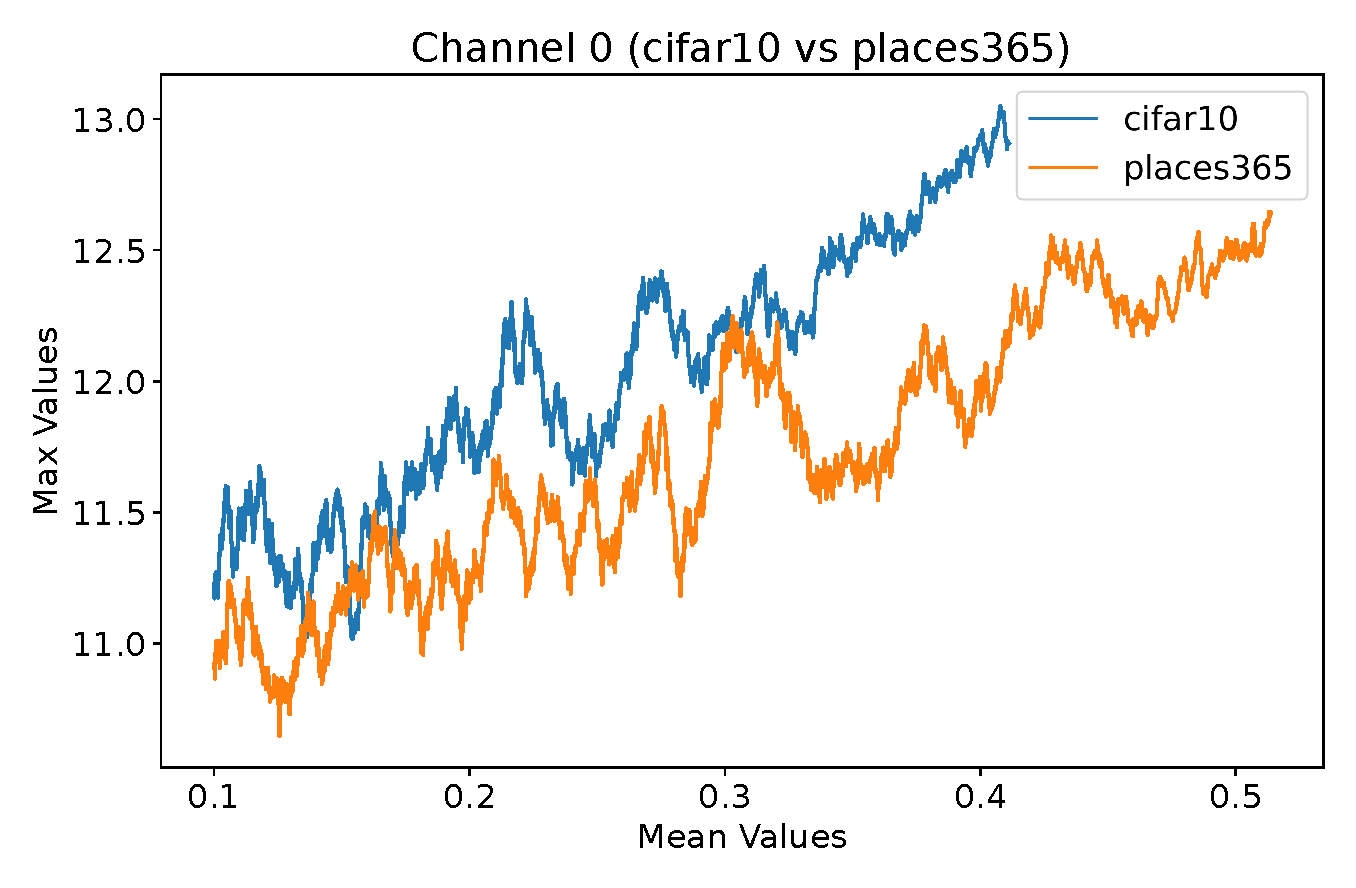
\includegraphics[width=0.24\linewidth]{eps/ap_p_0_channel_0.eps}
    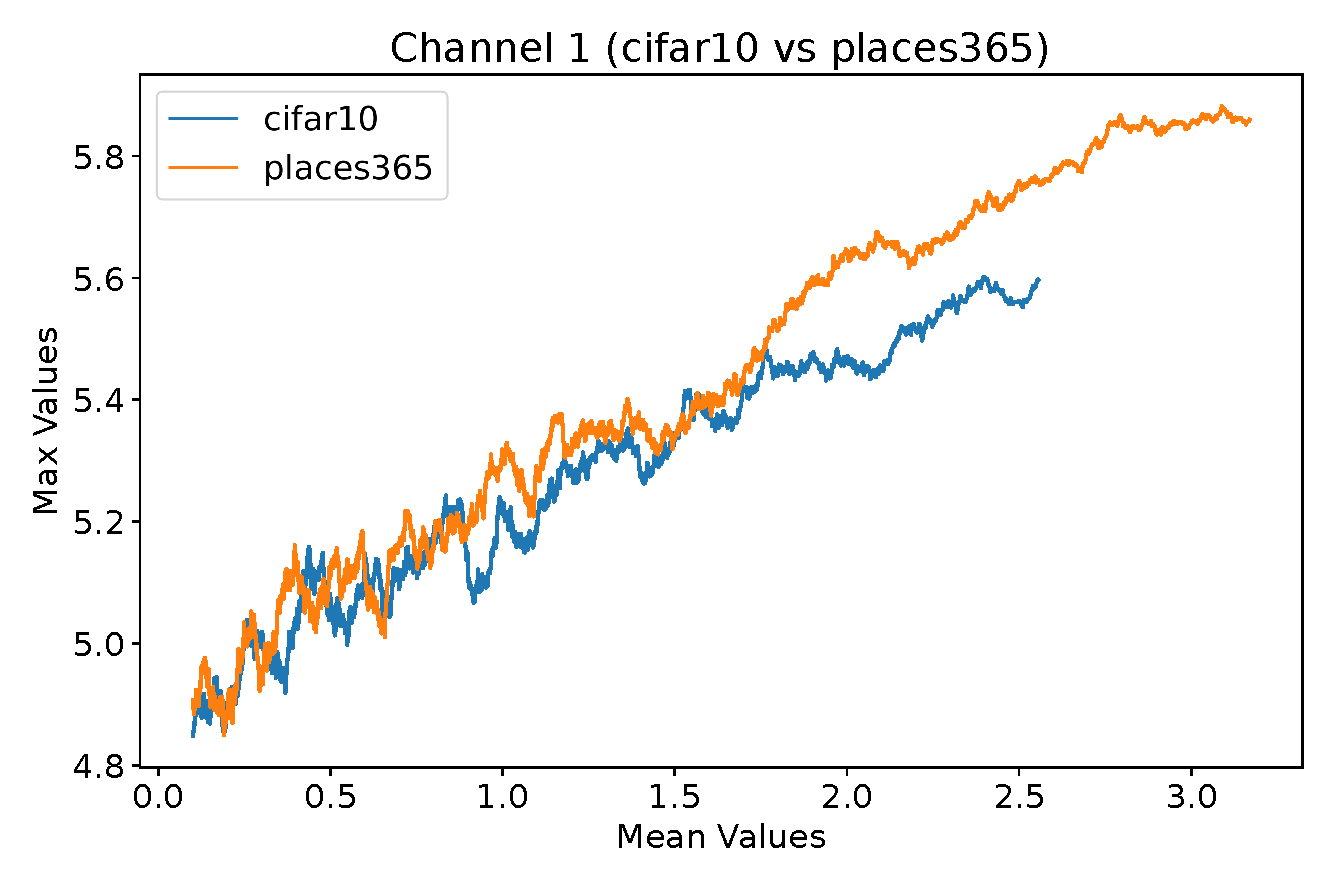
\includegraphics[width=0.24\linewidth]{eps/ap_p_0_channel_1.eps}
    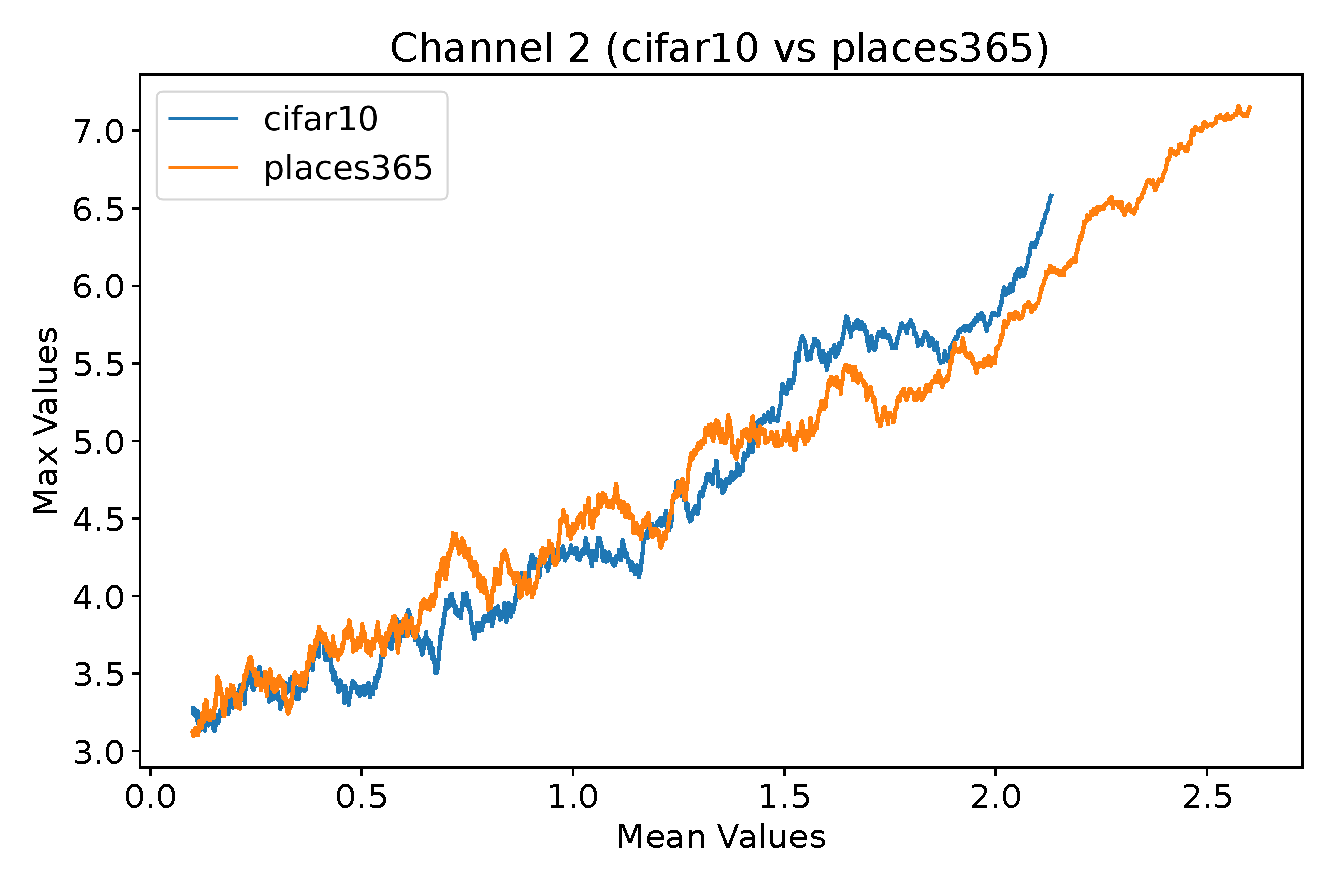
\includegraphics[width=0.24\linewidth]{eps/ap_p_0_channel_2.eps}
    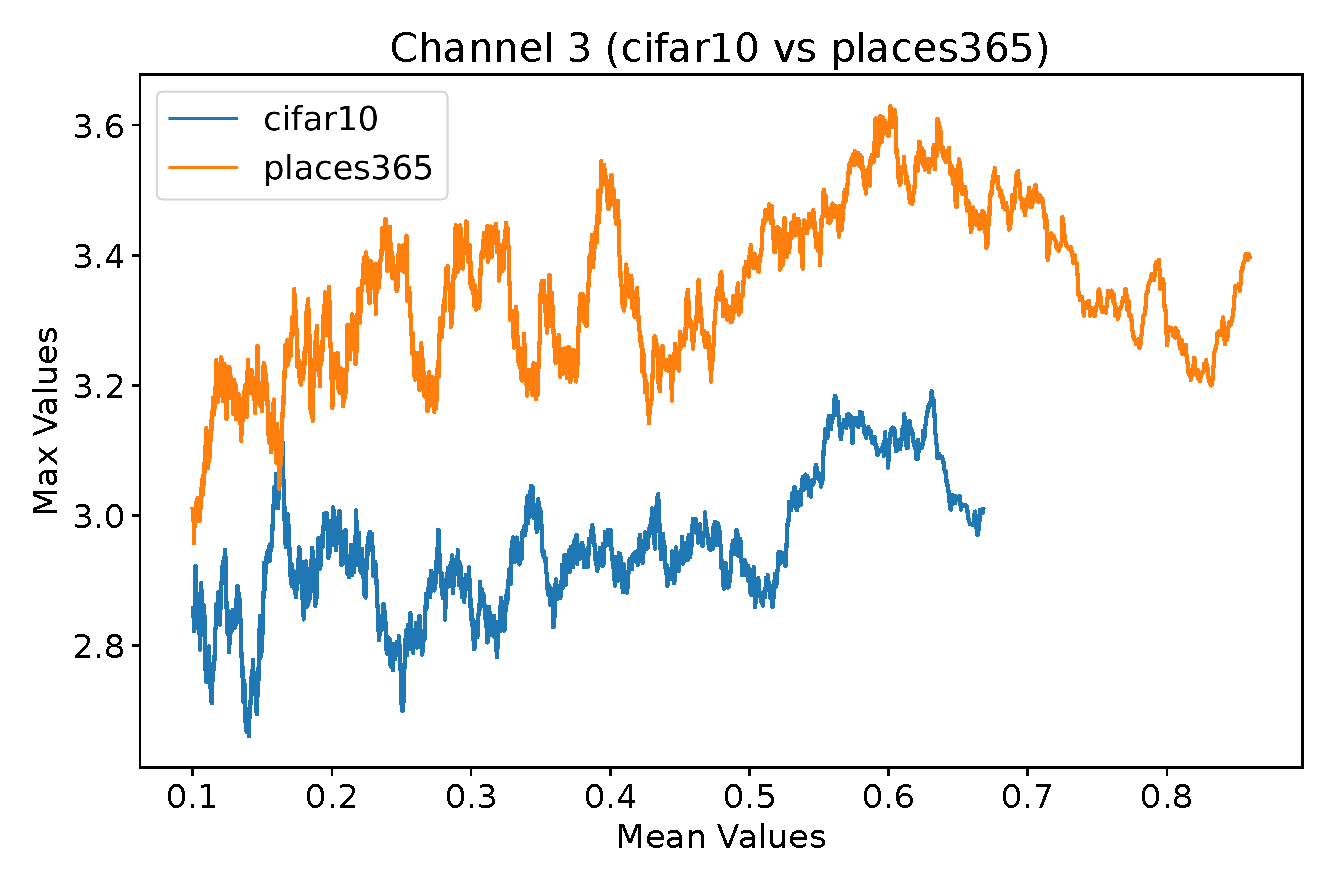
\includegraphics[width=0.24\linewidth]{eps/ap_p_0_channel_3.eps}
    \caption{After first convolution layer}
    \label{fig:places3650}
  \end{subfigure}

  \begin{subfigure}{\linewidth}
    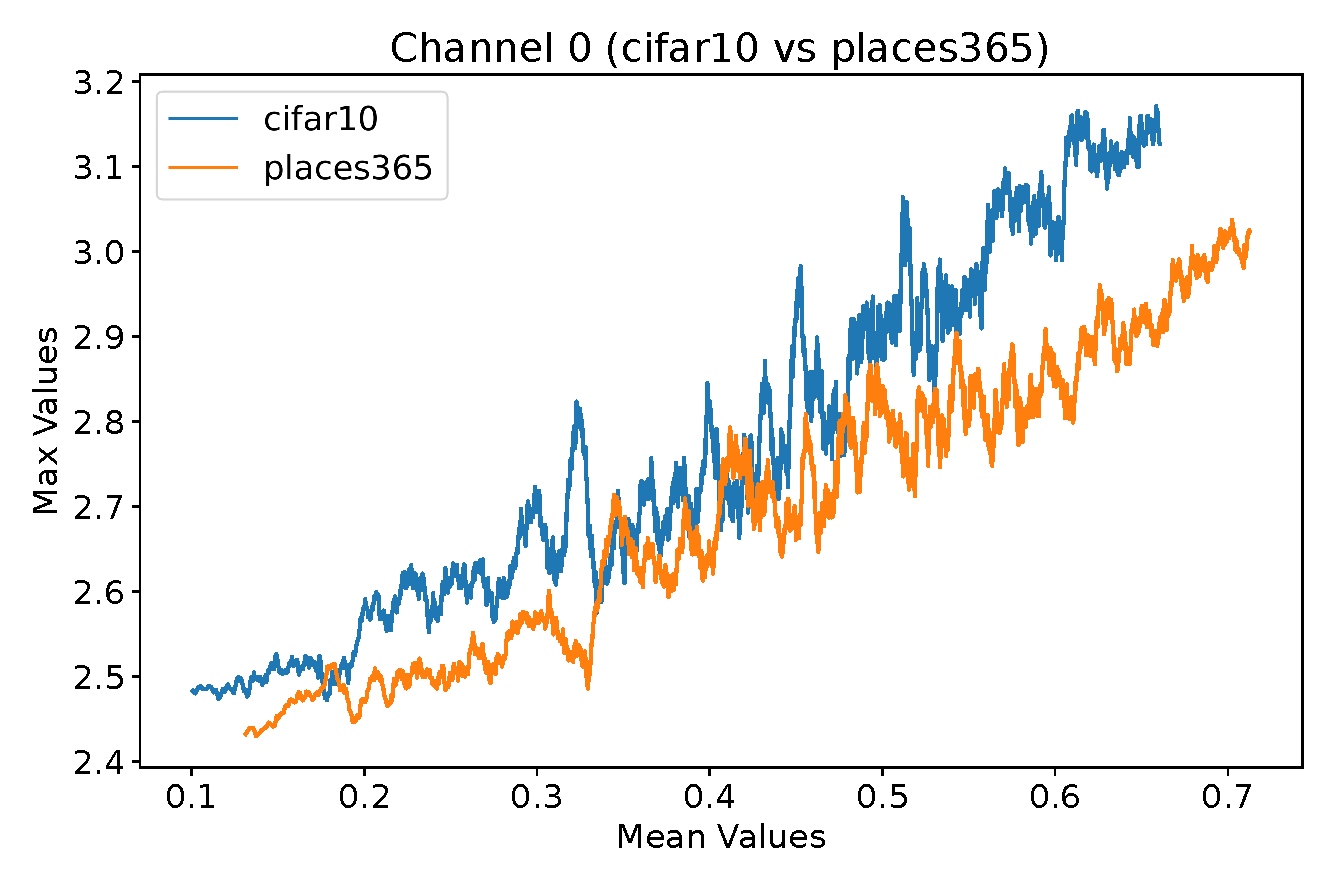
\includegraphics[width=0.24\linewidth]{eps/ap_p_1_channel_0.eps}
    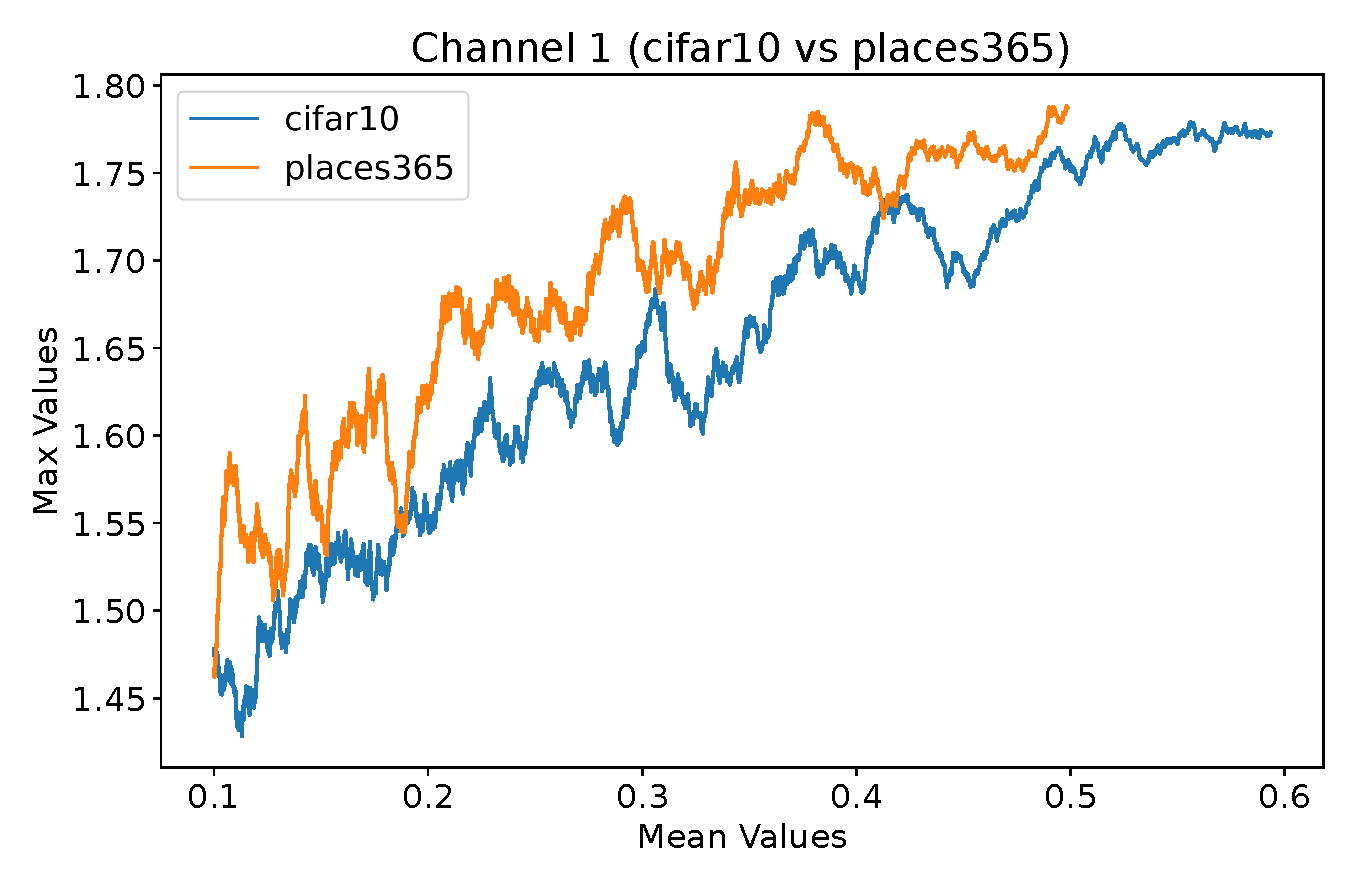
\includegraphics[width=0.24\linewidth]{eps/ap_p_1_channel_1.eps}
    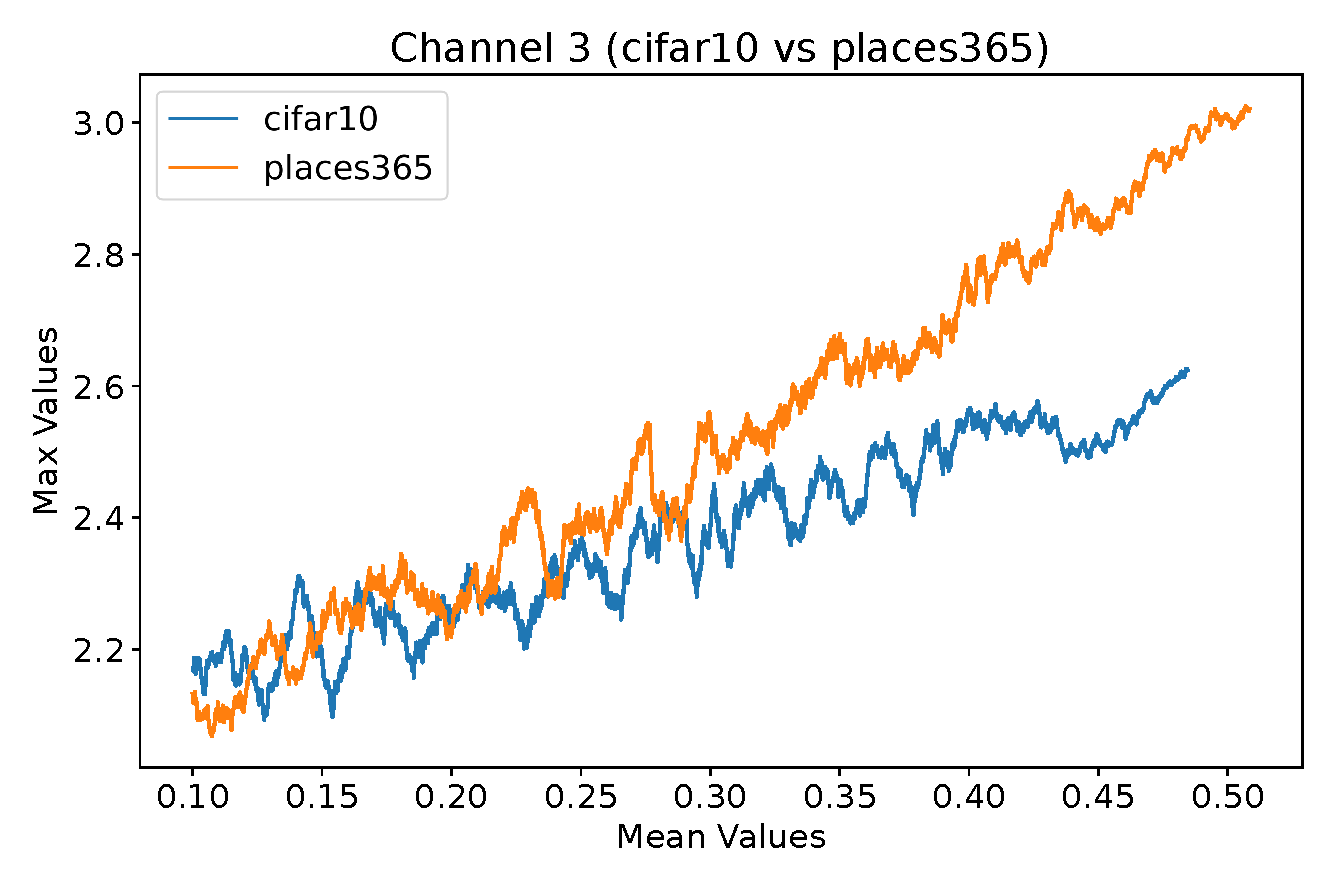
\includegraphics[width=0.24\linewidth]{eps/ap_p_1_channel_3.eps}
    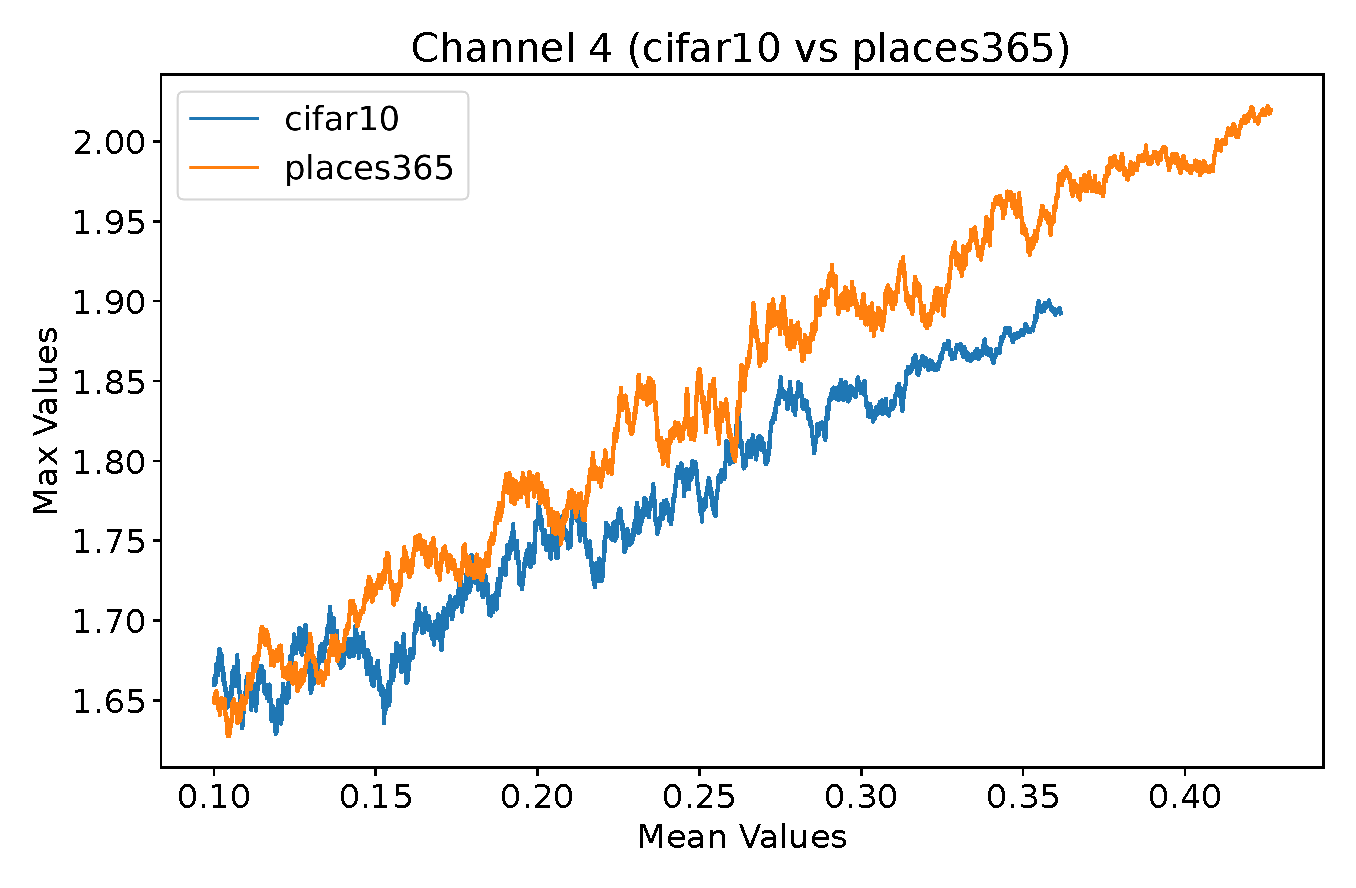
\includegraphics[width=0.24\linewidth]{eps/ap_p_1_channel_4.eps}
    \caption{In Transaction Block 1}
    \label{fig:places3651}
  \end{subfigure}

  \begin{subfigure}{\linewidth}
    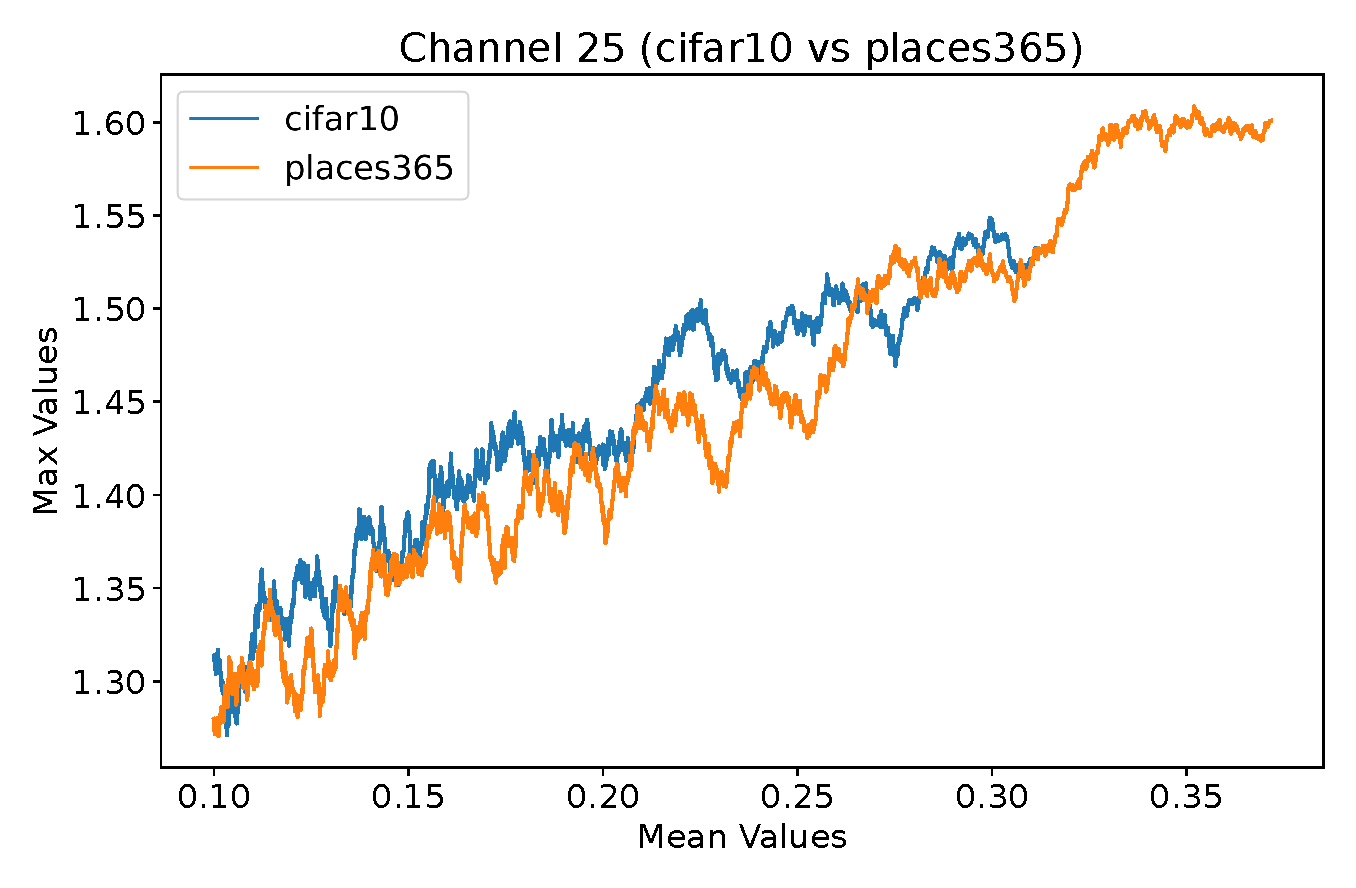
\includegraphics[width=0.24\linewidth]{eps/ap_p_2_channel_25.eps}
    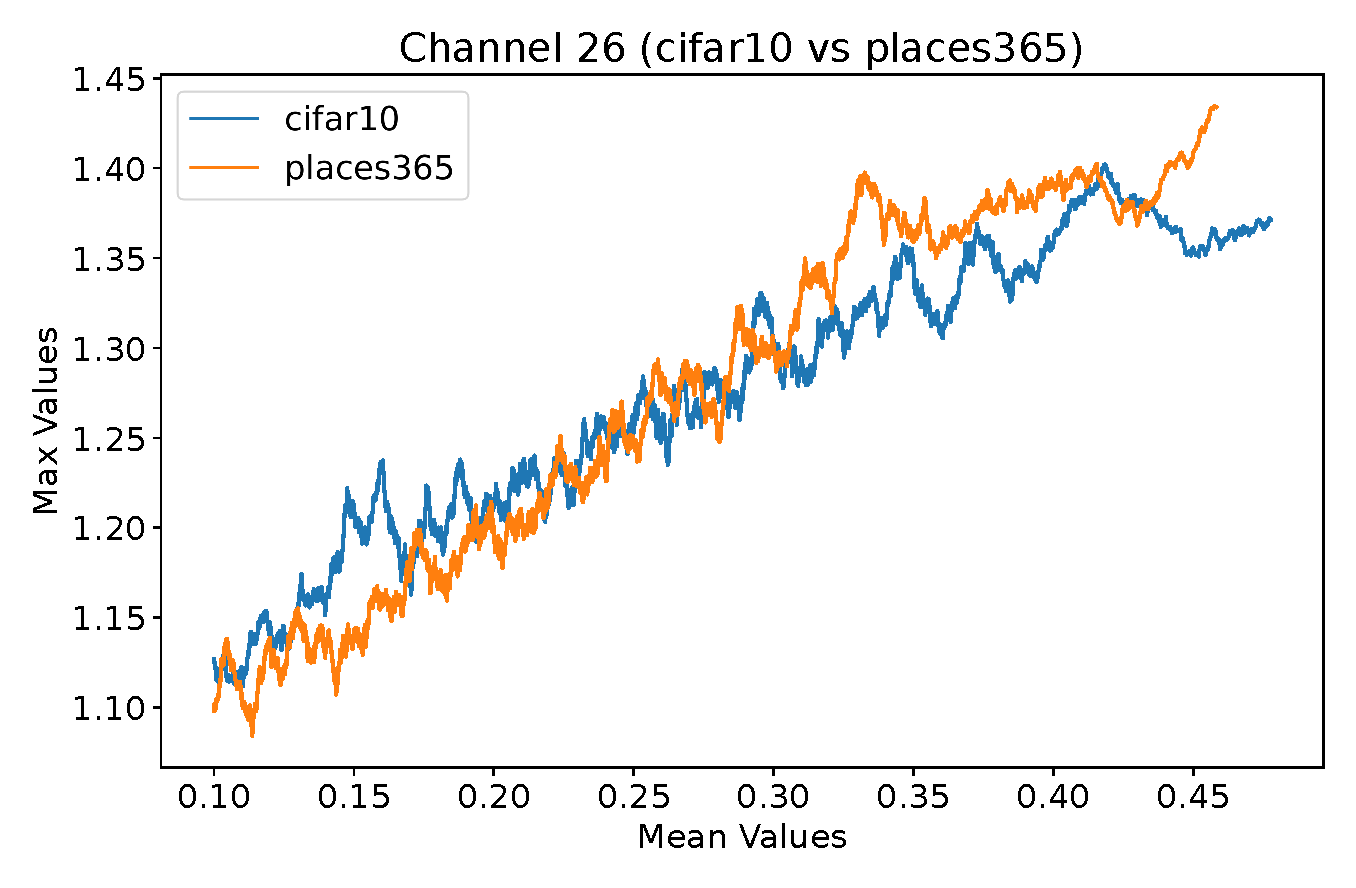
\includegraphics[width=0.24\linewidth]{eps/ap_p_2_channel_26.eps}
    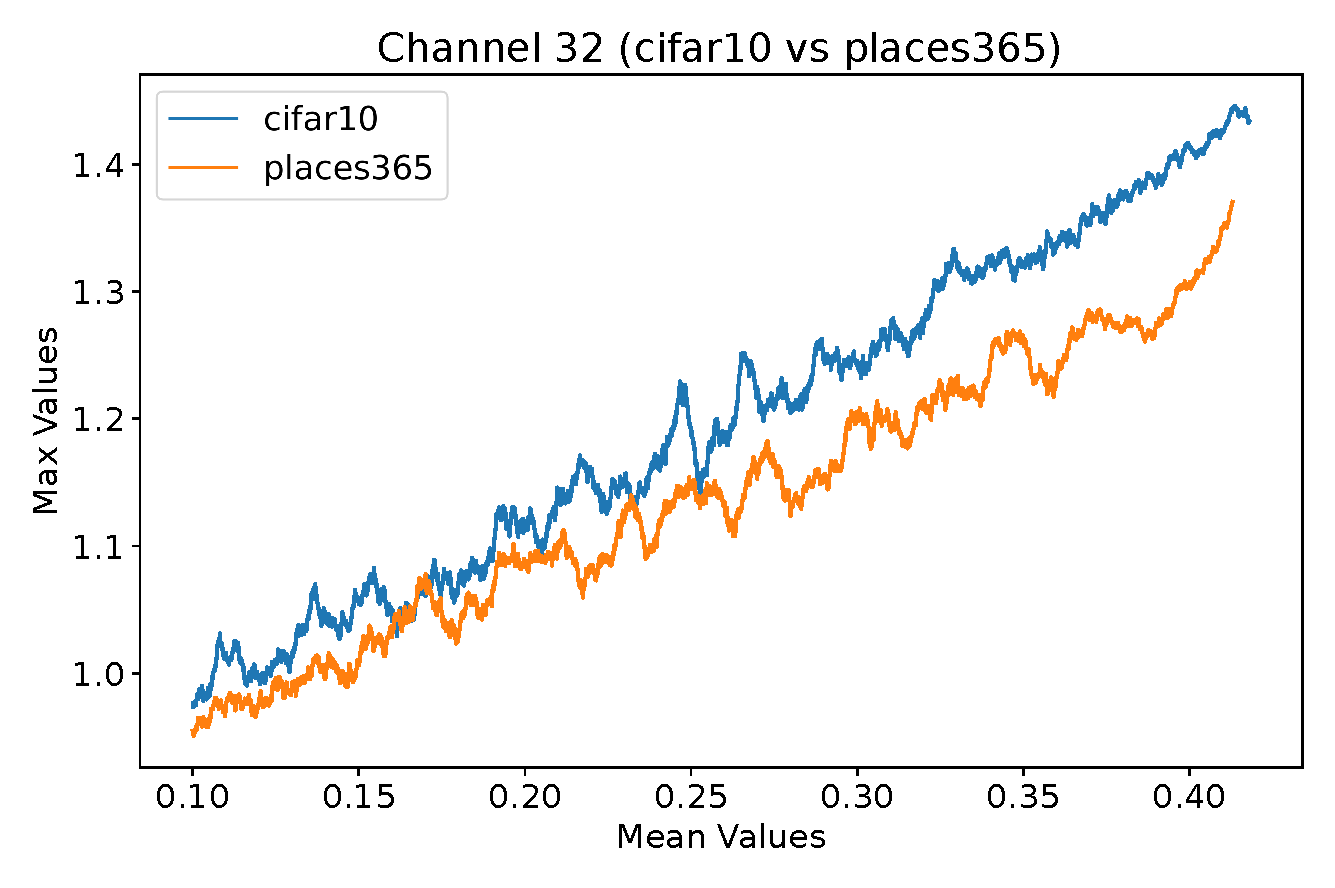
\includegraphics[width=0.24\linewidth]{eps/ap_p_2_channel_32.eps}
    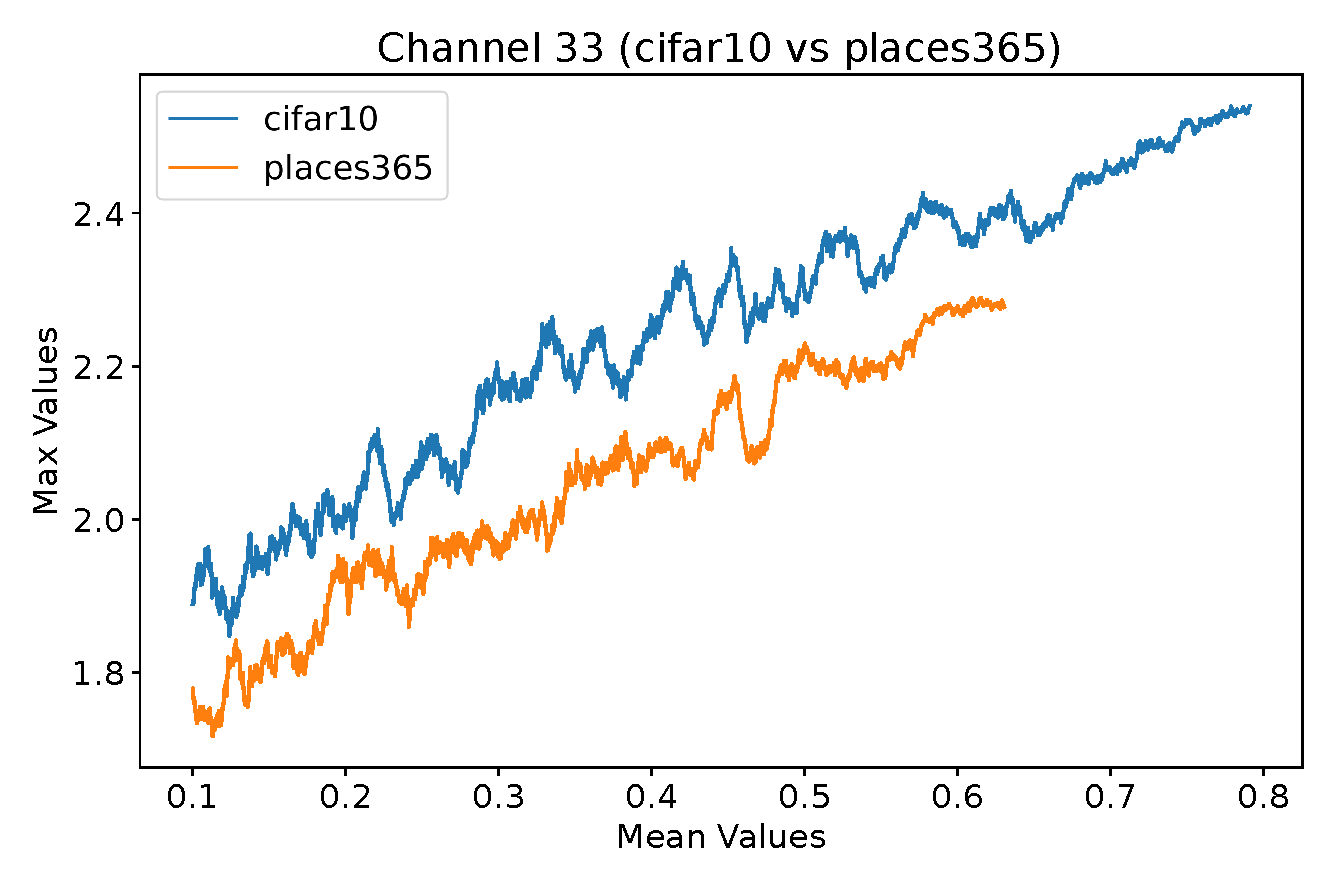
\includegraphics[width=0.24\linewidth]{eps/ap_p_2_channel_33.eps}
    \caption{In Transaction Block 2}
    \label{fig:places3652}
  \end{subfigure}

  \begin{subfigure}{\linewidth}
    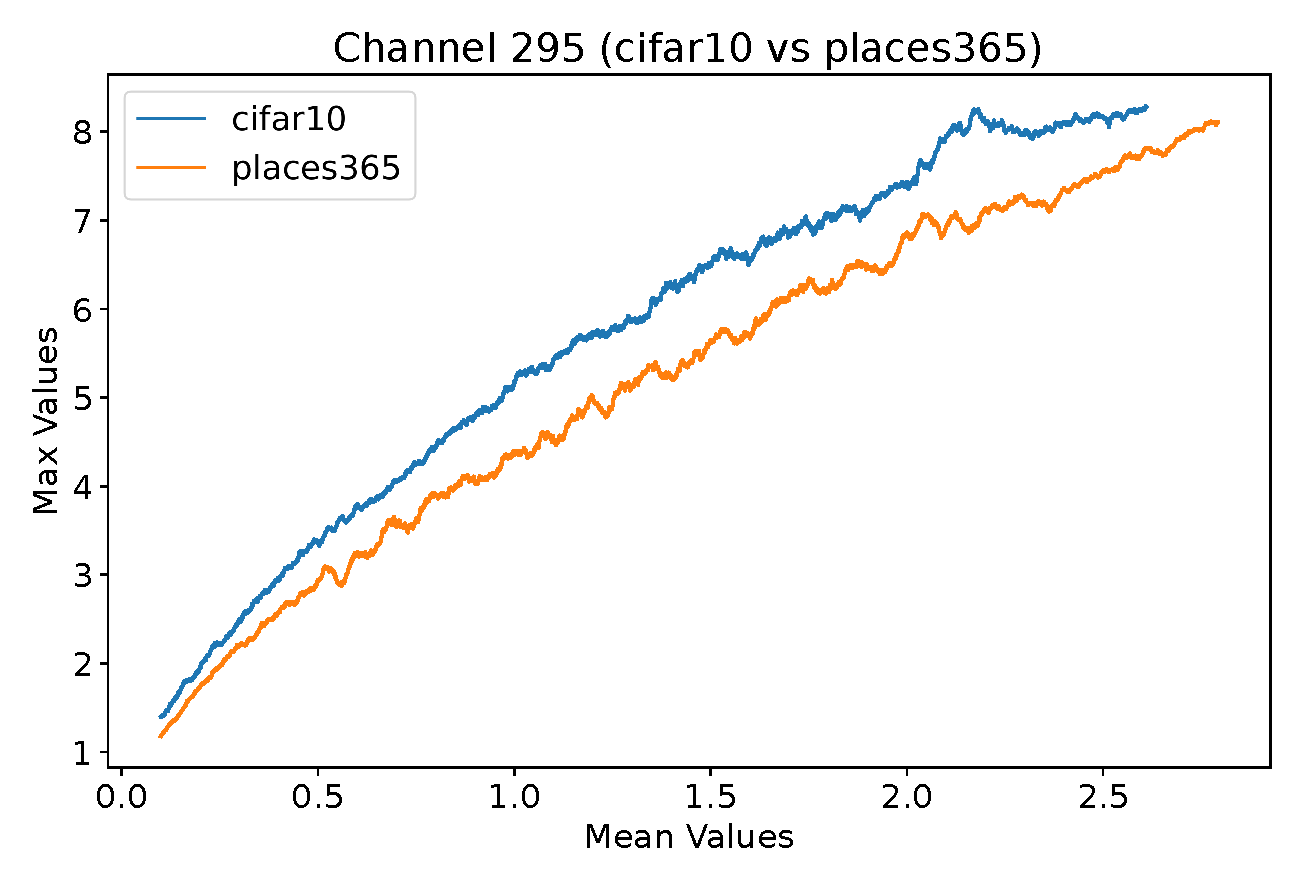
\includegraphics[width=0.24\linewidth]{eps/ap_p_3_channel_295.eps}
    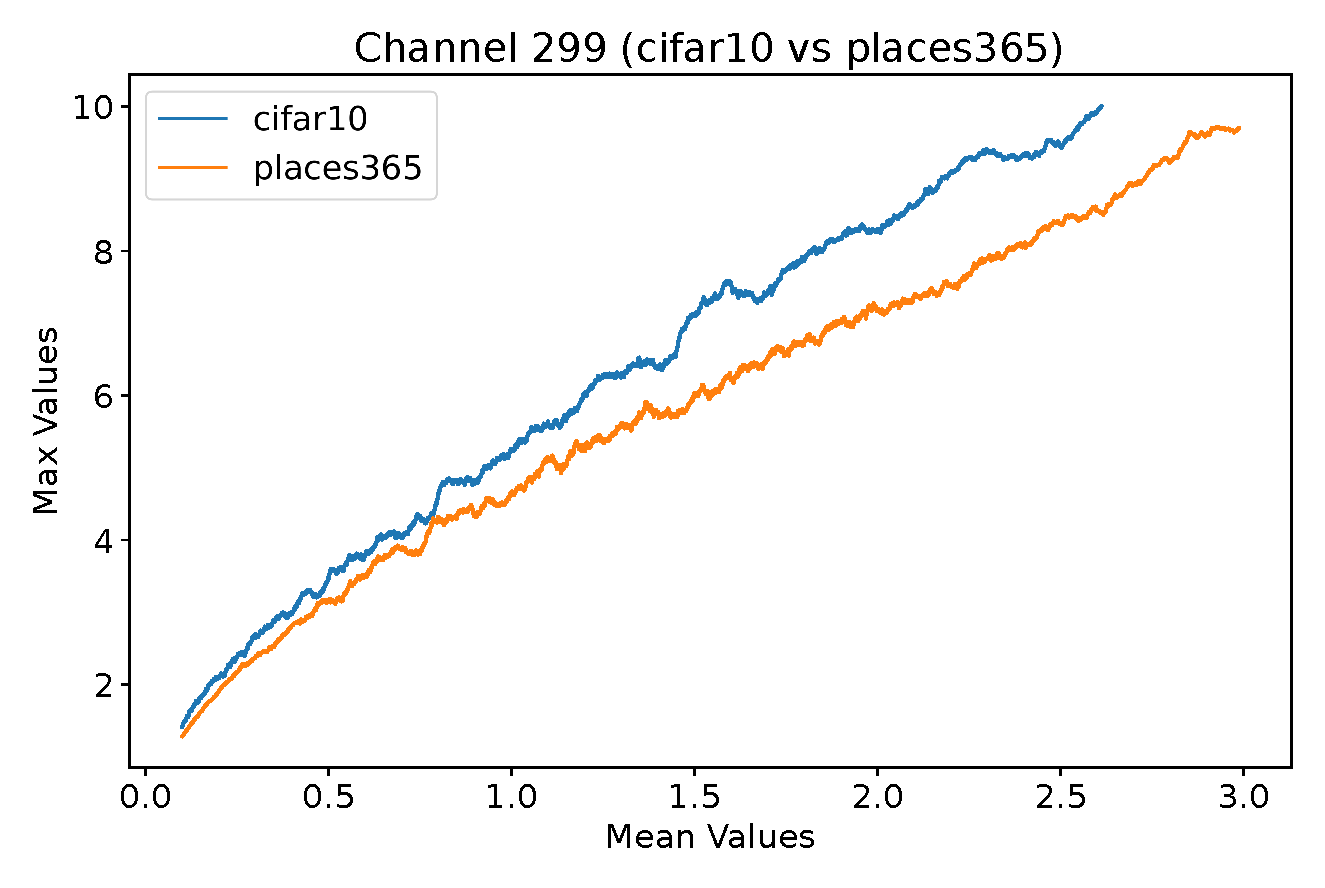
\includegraphics[width=0.24\linewidth]{eps/ap_p_3_channel_299.eps}
    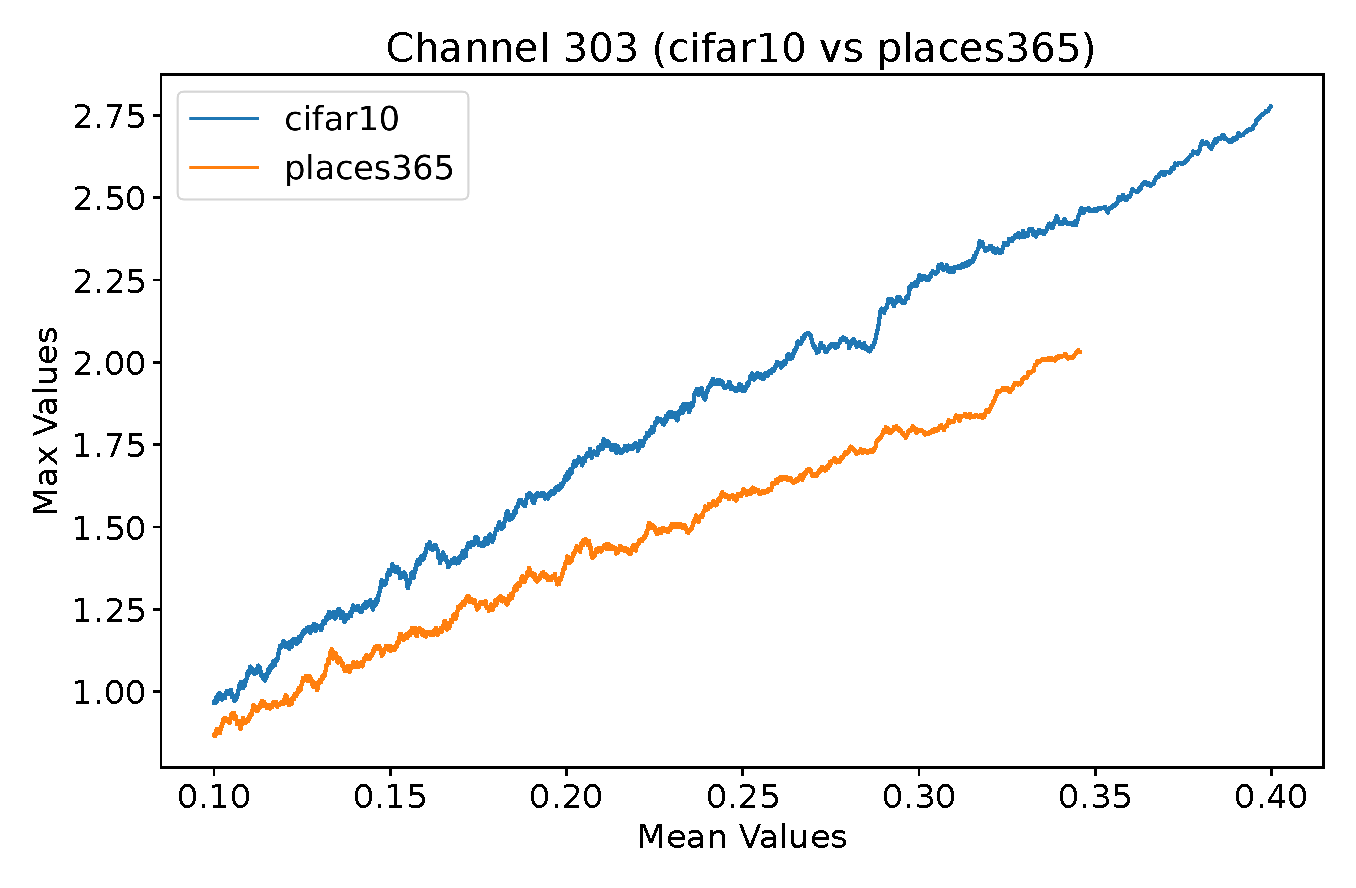
\includegraphics[width=0.24\linewidth]{eps/ap_p_3_channel_303.eps}
    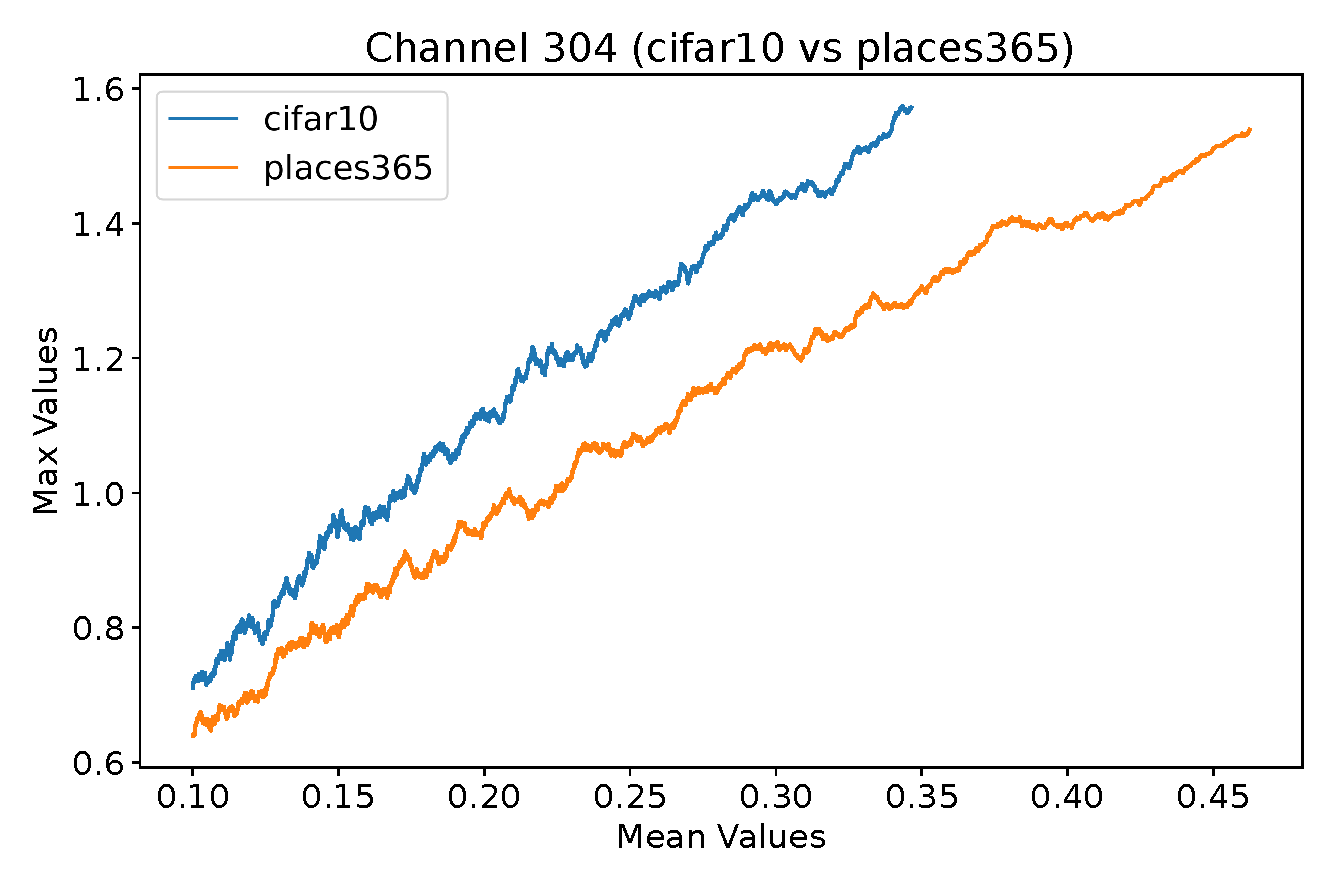
\includegraphics[width=0.24\linewidth]{eps/ap_p_3_channel_304.eps}
    \caption{Before Global Pooling}
    \label{fig:places3653}
  \end{subfigure}

  \caption{\textbf{Activation distribution at different positions within the DenseNet architecture~\cite{huang2017densely} applied to CIFAR-10 and Places365 datasets.} For this analysis, four specific locations within the network were chosen: (a) after the first convolution layer, (b) just before the pooling operation in the first transition block, (c) just before the pooling operation in the second transition block, and (d) right before the final global pooling layer. Note that we only include data points with an average activation over $0.1$. As shown in the figure, the first three selected layers show a less marked distinction between ID and OOD samples, while the fourth layer, preceding the final global pooling layer, demonstrates clearer separability and enhanced stability. Therefore, the fourth selected layer (the penultimate layer) is more suitable for developing a scoring function for OOD detection.}
  \label{fig:appendix-places365}
\end{figure}

\section{Why is the penultimate layer more effective for NAP?}
\label{appendix:layer}
We provide an extensive collection of visualizations showcasing the activations within the DenseNet architecture when applied to the CIFAR-10 (ID) dataset and Places365 (OOD) dataset. These visualizations are crucial for understanding how the network processes both ID and OOD data, revealing the distinct patterns of neural activations at various layers of the network.
Our analysis focuses on four critical layers within DenseNet: (1) after the first convolutional layer, (2) before the pooling operation in the first transition block, (3) before pooling in the second transition block, and (4) before the final global pooling layer. Each layer offers four visualizations, providing a comprehensive view of the network's response to different datasets.

These detailed visualizations enhance the discussion in the main text, offering deeper insights into how NAP effectively distinguishes between ID and OOD samples within the network. As depicted in Figure~\ref{fig:appendix-places365}, the first three selected layers, which focus primarily on low-level features, exhibit a less pronounced distinction between ID and OOD samples. This is likely because low-level features, such as edges and textures, are common to both ID and OOD datasets, making them less distinctive. However, the contrast between ID and OOD samples becomes more evident and stable in the fourth selected layer, located before the final global pooling layer. This layer, concentrating on high-level semantic information, captures features more unique to the ID dataset, leading to clearer separability and enhanced stability in activation values compared to earlier layers. This layer's focus on distinctive semantic features makes it particularly suitable for developing a scoring function for OOD detection. 
Therefore, since the penultimate layer is the most informative layer in the neural network, we utilize this layer in our method to develop our scoring function.
%%%%%%%%%%%%%%%%%%%%%%%%%%%%%%%%%%%%%%%%%%%%%%%%%%%%%%%%%%%%%%%%%%%%%%%%%%%
\begin{table}[!t]
\footnotesize
\centering
\caption{\textbf{Experimental results of OOD detection using NAP at different layers in DenseNet~\cite{huang2017densely} on CIFAR-10 and CIFAR-100 datasets.} NAP(x) indicates the computation of OOD score at the layer 'x', where 'c1' corresponds to after the first convolutional layer, 't1' before the pooling operation in the first transition block, 't2' before pooling in the second transition block, and 'p' before the final global pooling layer. Combinations of layers, indicated by commas in NAP(..), represent the multiplication of OOD scores from respective layers. These selected layers are consistent with those used for visualizations described earlier in the paper. Notably, NAP(p) is the approach actually utilized in our paper.\\}
% \tabcolsep=0.4cm
\label{tab:multi-layer}
\begin{tabular}{@{}lcc|cc@{}}
\toprule
\multirow{2}{*}{\textbf{Method}} & \multicolumn{2}{c|}{\textbf{CIFAR-10}} & \multicolumn{2}{c}{\textbf{CIFAR-100}} \\ \cmidrule{2-5} 
                                 & FPR95              & AUROC             & FPR95              & AUROC             \\ \midrule
NAP(c1)                          & 83.22              & 51.99             & 84.13              & 50.34             \\
NAP(t1)                          & 69.10              & 50.47             & 86.82              & 54.92             \\
NAP(t2)                          & 56.53              & 78.44             & 88.85              & 53.08             \\
NAP(c1,t1,t2,p)                  & 68.33              & 58.99             & 82.66              & 56.96             \\
NAP(t1,t2,p)                     & 56.84              & 64.26             & 83.35              & 57.97             \\
NAP(t2,p)                        & 34.41              & 87.81             & 82.74              & 58.31             \\
\textbf{NAP(p)}                  & \textbf{26.57}     & \textbf{92.45}    & \textbf{54.91}     & \textbf{85.86}    \\ \bottomrule
\end{tabular}
\end{table}

\section{Evaluating multi-layer integration with NAP for OOD detection}
\label{appendix:integration}
In an additional exploration presented in the appendix, we investigate the effects of incorporating values from both the penultimate layer and earlier layers on OOD detection. Our experiments, detailed in Table~\ref{tab:multi-layer}, suggest that the integration of earlier layers with the penultimate layer, where NAP is primarily applied, does not yield significant improvements in OOD detection. This phenomenon could partly stem from the inherent limitations of earlier layers in differentiating between ID and OOD data. Additionally, there is a possibility that the scoring function, specifically optimized for the penultimate layer, may not align optimally with the feature representation characteristics of the preceding layers. Considering the constraints of space in this paper, a comprehensive analysis of multi-layer integration using NAP is not presented. Nonetheless, the potential of combining multiple layers in OOD detection, especially in the context of NAP, remains an intriguing aspect for future research. We anticipate that further investigations, potentially involving the creation of new scoring functions suitable for a broader range of layers, could provide substantial contributions to the field. Thus, we propose this as an avenue for future work, aiming to stimulate further advancements within the research community.
%%%%%%%%%%%%%%%%%%%%%%%%%%%%%%%%%%%%%%%%%%%%%%%%%%%%%%%%%%%%%%%%%%%%%%%%%%%
\section{On transferability to other architectures}
\label{appendix:transfer}
In Figure~\ref{fig:appendix-e-mobilenet}, \ref{fig:appendix-e-resnet}, and \ref{fig:appendix-e-vgg}, we present detailed visualizations of the activation patterns within three distinct architectures: MobileNetV2~\cite{sandler2018mobilenetv2}, ResNet50~\cite{he2016deep}, and VGG16~\cite{simonyan2015very}. These visualizations clearly demonstrate a remarkable gap between ID samples, depicted with blue lines, and OOD samples, represented with orange lines. This distinction is evident across all three architectures, underscoring the versatility and effectiveness of the proposed NAP. The consistent separability observed in these diverse architectures confirms the adaptability and potential of NAP for broad application in different neural network models.

In order to validate the effectiveness of NAP across different Convolutional Neural Network (CNN) architectures, we conducted experiments on a variety of CNN backbones. As depicted in Table~\ref{tab:backbones}, our proposed NAP method significantly enhances the OOD detection performance across various CNN structures.
These results underscore the adaptability of NAP to various CNN models, demonstrating its potential as a versatile tool for enhancing the reliability and accuracy of OOD detection in neural network applications. 
\begin{table}[!h]
\scriptsize
\centering
\caption{Results on ImageNet with various backbones.\\\quad\\}
\label{tab:backbones}
% \tabcolsep=0.3cm
\begin{tabular}{@{}lcc|cc|cc@{}}
\toprule
             & \multicolumn{2}{c|}{Energy} & \multicolumn{2}{c|}{NAP} & \multicolumn{2}{c}{NAP-E} \\ \cmidrule(l){2-7} 
             & FPR95        & AUROC        & FPR95       & AUROC      & FPR95       & AUROC       \\ \midrule
VGG          & 54.34             & 88.17             &  29.23           & 93.46           & \textbf{23.23}            & \textbf{95.00}            \\
DenseNet      & 50.40             & 87.66             & 49.89            & 88.40           & \textbf{32.95}            & \textbf{91.68}            \\
ResNet    & 57.47             & 87.05             & 48.77            & 82.76           & \textbf{32.12}            & \textbf{92.02}            \\ \bottomrule
\end{tabular}
% \vspace{-12pt}
\end{table}
%%%%%%%%%%%%%%%%%%%%%%%%%%%%%%%%%%%%%%%%%%%%%%%%%%%%%%%%%%%%%%%%%%%%%%%%%%%
\section{Pareto frontier of ID accuracy and OOD detection performance}
\label{appendix:pareto}
\begin{figure}[!h]
% \vspace{-15pt}
  \centering
  \begin{subfigure}{0.47\linewidth}
    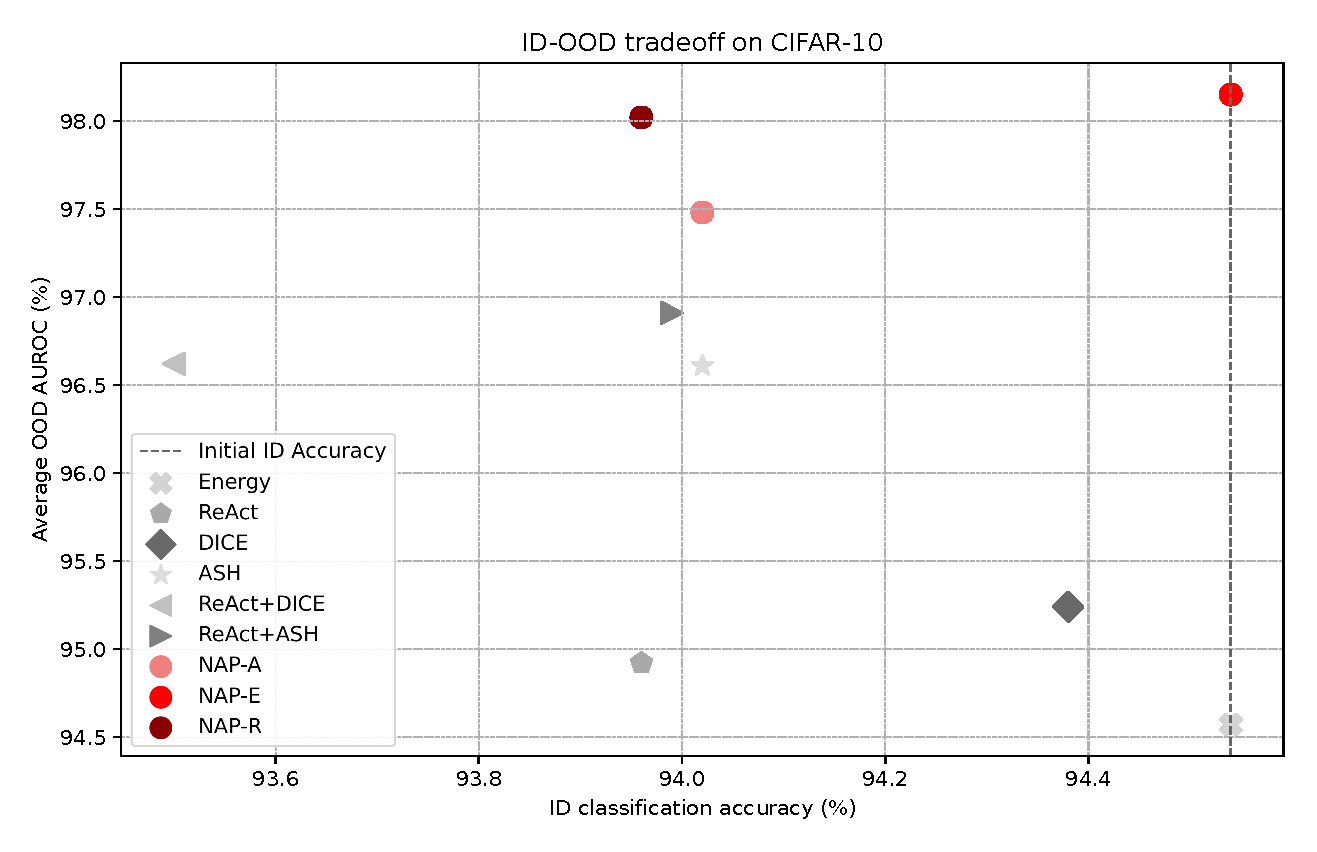
\includegraphics[width=0.99\linewidth]{eps/pareto_cifar10.eps}
    \caption{CIFAR-10}
    \label{fig:p1}
  \end{subfigure}
  \hfill
  \begin{subfigure}{0.46\linewidth}
    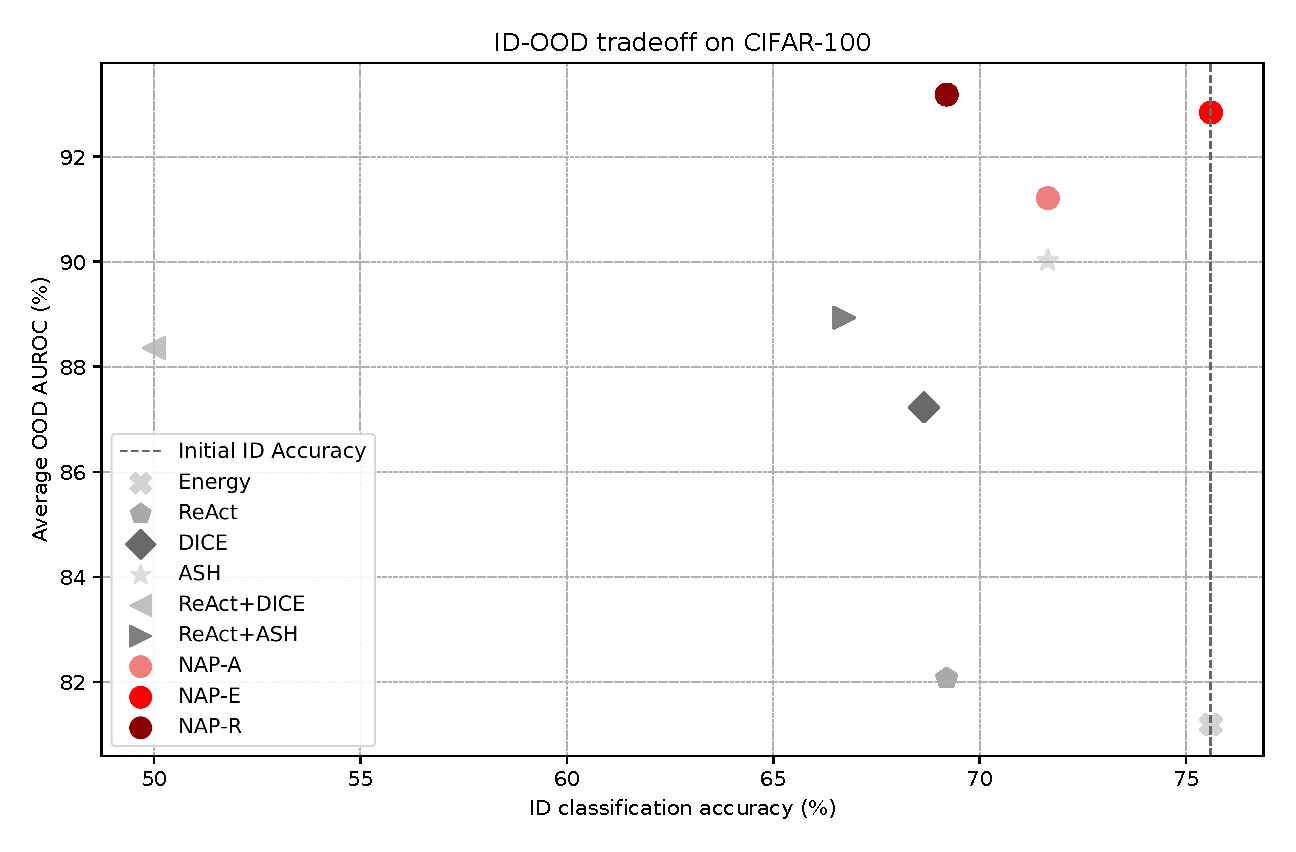
\includegraphics[width=0.99\linewidth]{eps/pareto_cifar100.eps}
    \caption{CIFAR-100}
    \label{fig:p2}
  \end{subfigure}
  \caption{\textbf{Investigating the trade-offs between ID classification accuracy and OOD detection AUROC on CIFAR benchmarks~\cite{krizhevsky2009cifar} across various methods.} All methods and experiments are implemented by us. Methods prefixed with 'NAP' are visually distinguished, highlighted in various shades of red in the figures.}
  \label{fig:pareto-cifar}
\end{figure}
Some existing methods negatively affect ID accuracy; however, we have found that integrating these methods with the NAP approach can mitigate or reduce this impact, achieving a more optimal balance. The NAP approach establishes an ideal equilibrium between ID classification accuracy and OOD detection efficacy (measured in AUROC), thereby positioning it favorably on the Pareto front for superior performance. This demonstrates our method's ability to enhance OOD detection without additional costs while maintaining the model’s classification performance, as illustrated in Figures~\ref{fig:p1} and ~\ref{fig:p2} using the CIFAR benchmark~\cite{krizhevsky2009cifar}.
%%%%%%%%%%%%%%%%%%%%%%%%%%%%%%%%%%%%%%%%%%%%%%%%%%%%%%%%%%%%%%%%%%%%%%%%%%%
\section{Full CIFAR benchmark results: enhancing methods with NAP}
\label{appendix:cifar}
This section focuses on the significant enhancements brought by the Neural Activation Prior (NAP) to existing out-of-distribution detection methods in the context of the CIFAR-10 (in Table~\ref{tab:cifar10}) and CIFAR-100 (in Table~\ref{tab:cifar100}) dataset. The incorporation of NAP into established methods like Energy~\cite{liu2020energy}, ASH~\cite{djurisic2022extremely}, DICE~\cite{sun2022dice}, KNN~\cite{sun2022knn}, MSP~\cite{hendrycks2016msp} and ReAct~\cite{sun2021react}, resulting in \textbf{NAP-E}, \textbf{NAP-A}, \textbf{NAP-D}, \textbf{NAP-K}, \textbf{NAP-M}and \textbf{NAP-R} respectively, showcases the potential of NAP in augmenting existing approaches.
Our experimental results demonstrate that NAP-based variants consistently outperform their corresponding traditional methods across all six OOD datasets. Notably, our experimental results reveal some extremely substantial decreases in FPR95 values, indicative of the profound impact of NAP integration. For instance, on the CIFAR-100 dataset, the FPR95 value of NAP-R, compared to ReAct, dropped by 83.06\% (from 83.81 to 14.19), highlighting a notable reduction in false alarms while maintaining high detection accuracy and affirming the enhanced capability of these methods in distinguishing between in-distribution and OOD samples.

\begin{table}[!h]
\tiny
\centering
\caption{\textbf{Scoring function proposed based on NAP is compatible with and improves on existing methods on CIFAR-10 dataset.}  All methods and experiments are implemented by us. All values in this table are percentages. The average over six OOD test datasets is also reported. The methods with prefix 'NAP-' (e.g., NAP-E, NAP-A, NAP-R) represent the integration of NAP with various existing methods (Energy~\cite{liu2020energy}, ASH-S~\cite{djurisic2022extremely}, ReAct~\cite{sun2021react} respectively).\\}
\label{tab:cifar10}
\resizebox{\textwidth}{!}{
\begin{tabular}{LcccccccccccccR}
\toprule
\multicolumn{1}{c}{\multirow{3}{*}{\textbf{Method}}} & \multicolumn{12}{c}{\textbf{OOD Datasets}}                                                                                                                                                                                                                                                                                                    & \multicolumn{2}{c}{\multirow{2}{*}{\textbf{Average}}} \\ \cline{2-13}
\multicolumn{1}{c}{}                                 & \multicolumn{2}{c}{\textbf{SVHN}}                     & \multicolumn{2}{c}{\textbf{Textures}}                 & \multicolumn{2}{c}{\textbf{iSUN}}                     & \multicolumn{2}{c}{\textbf{LSUN}}                     & \multicolumn{2}{c}{\textbf{LSUN-Crop}}                & \multicolumn{2}{c}{\textbf{Places365}}                & \multicolumn{2}{c}{}                                  \\
\multicolumn{1}{c}{}                                 & \multicolumn{1}{c}{FPR95} & \multicolumn{1}{c}{AUROC} & \multicolumn{1}{c}{FPR95} & \multicolumn{1}{c}{AUROC} & \multicolumn{1}{c}{FPR95} & \multicolumn{1}{c}{AUROC} & \multicolumn{1}{c}{FPR95} & \multicolumn{1}{c}{AUROC} & \multicolumn{1}{c}{FPR95} & \multicolumn{1}{c}{AUROC} & \multicolumn{1}{c}{FPR95} & \multicolumn{1}{c}{AUROC} & \multicolumn{1}{c}{FPR95} & \multicolumn{1}{c}{AUROC} \\ \hline
ASH                            & 6.51                      & 98.65                     & 24.34                     & 95.09                     & 5.17                      & 98.90                     & 4.96                      & 98.92                     & 0.90                      & 99.73                     & 48.45                     & 88.34                     & 15.05                     & 96.91                     \\ 
\rowcolor[HTML]{C0C0C0}
\textbf{NAP-A}            & 5.55                      & 98.86                     & 10.51                     & 97.90                     & 3.04                      & 99.32                     & 2.68                      & 99.40                     & 0.80                      & 99.80                     & 44.28                     & 89.59                     & 11.14                     & 97.48                    \\ % \midrule
DICE                      & 29.62                     &      94.66                     & 0.38                      &      99.90                     & 4.43                      &      99.03                     & 5.14                      &      98.97                     & 45.87                     &      86.97                     & 45.32                     &      90.29                     & 21.79                     &      94.97                 \\
\rowcolor[HTML]{C0C0C0}
\textbf{NAP-D}            & 10.60                      &     97.75                     & 0.41                       &     99.88                     & 2.03                       &     99.48                     & 2.69                       &     99.41                     & 13.85                      &     96.98                     & 40.40                      &     91.31                     & 11.66                      &     97.47                  \\ % \midrule
Energy                           & 40.57                     & 93.99                     & 56.29                     & 86.42                     & 10.07                     & 98.07                     & 9.28                      & 98.12                     & 3.81                      & 99.15                     & 39.50                     & 92.01                     & 26.59                     & 94.63                     \\
\rowcolor[HTML]{C0C0C0}
\textbf{NAP-E}            & 8.32                      & 98.36                     & 11.65                     & 97.72                     & 1.77                      & 99.57                     & 1.50                      & 99.60                     & 0.99                      & 99.76                     & 29.89                     & 93.91                     & 9.02                      & 98.15                     \\ % \midrule
KNN                       & 4.31                      &      99.20                     & 7.71                      &      98.62                     & 9.45                      &      98.22                     & 10.08                     &      98.15                     & 19.31                     &      96.46                     & 45.83                     &      90.09                     & 16.12                     &      96.79                 \\
\rowcolor[HTML]{C0C0C0}
\textbf{NAP-K}            & 2.39                      &      99.56                     & 2.29                      &      99.55                     & 1.76                      &      99.57                     & 2.45                      &      99.47                     & 3.58                      &      99.34                     & 34.27                     &      92.80                     & 7.79                      &      98.38                 \\ % \midrule
MSP                       & 47.34                     &      93.48                     & 33.66                     &      95.54                     & 42.21                     &      94.51                     & 42.42                     &      94.52                     & 64.52                     &      88.14                     & 61.98                     &      88.95                     & 48.69                     &      92.52                 \\
\rowcolor[HTML]{C0C0C0}
\textbf{NAP-M}            & 14.09                     &      96.05                     & 7.33                      &      98.35                     & 10.91                     &      97.72                     & 11.20                     &      97.55                     & 16.42                     &      96.23                     & 54.61                     &      84.76                     & 19.09                     &      95.11                 \\ % \midrule
ReAct                            & 41.64                     & 93.87                     & 43.58                     & 92.47                     & 12.72                     & 97.72                     & 11.46                     & 97.87                     & 5.96                      & 98.84                     & 43.31                     & 91.03                     & 26.45                     & 94.67                     \\
\rowcolor[HTML]{C0C0C0}
\textbf{NAP-R}            & 8.07                      & 98.31                     & 8.10                      & 98.17                     & 2.81                      & 99.35                     & 2.35                      & 99.43                     & 3.04                      & 99.33                     & 30.70                     & 93.50                     & 9.18                      & 98.02                    \\ \bottomrule
\end{tabular}
}
\end{table}

\begin{table}[!h]
\tiny
\centering
\caption{\textbf{Scoring function proposed based on NAP is compatible with and improves on existing methods on CIFAR-100 dataset.}  All methods and experiments are implemented by us. All values in this table are percentages. The average over six OOD test datasets is also reported. The methods with prefix 'NAP-' (e.g., NAP-E, NAP-A, NAP-R) represent the integration of NAP with various existing methods (Energy~\cite{liu2020energy}, ASH-S~\cite{djurisic2022extremely}, ReAct~\cite{sun2021react} respectively).\\}
\label{tab:cifar100}
\resizebox{\textwidth}{!}{
\begin{tabular}{LcccccccccccccR}
\toprule
\multicolumn{1}{c}{\multirow{3}{*}{\textbf{Method}}} & \multicolumn{12}{c}{\textbf{OOD Datasets}}                                                                                                                                                                                                                                                                                                    & \multicolumn{2}{c}{\multirow{2}{*}{\textbf{Average}}} \\ \cline{2-13}
\multicolumn{1}{c}{}                                 & \multicolumn{2}{c}{\textbf{SVHN}}                     & \multicolumn{2}{c}{\textbf{Textures}}                 & \multicolumn{2}{c}{\textbf{iSUN}}                     & \multicolumn{2}{c}{\textbf{LSUN}}                     & \multicolumn{2}{c}{\textbf{LSUN-Crop}}                & \multicolumn{2}{c}{\textbf{Places365}}                & \multicolumn{2}{c}{}                                  \\
\multicolumn{1}{c}{}                                 & \multicolumn{1}{c}{FPR95} & \multicolumn{1}{c}{AUROC} & \multicolumn{1}{c}{FPR95} & \multicolumn{1}{c}{AUROC} & \multicolumn{1}{c}{FPR95} & \multicolumn{1}{c}{AUROC} & \multicolumn{1}{c}{FPR95} & \multicolumn{1}{c}{AUROC} & \multicolumn{1}{c}{FPR95} & \multicolumn{1}{c}{AUROC} & \multicolumn{1}{c}{FPR95} & \multicolumn{1}{c}{AUROC} & \multicolumn{1}{c}{FPR95} & \multicolumn{1}{c}{AUROC} \\ \hline
ASH                                                 & 25.02                     & 95.76                     & 34.02                     & 92.35                     & 46.67                     & 91.30                     & 51.33                     & 90.12                     & 5.52                      & 98.84                     & 85.86                     & 71.62                     & 41.40                     & 90.02                     \\
\rowcolor[HTML]{C0C0C0}
\textbf{NAP-A}                                 & 17.41                     & 96.72                     & 22.70                     & 94.99                     & 38.22                     & 93.34                     & 43.05                     & 92.17                     & 5.25                      & 98.94                     & 85.76                     & 72.08                     & 35.40                     & 91.32                     \\
DICE                           & 59.25                      & 88.57                      & 0.91                      & 99.74                        & 51.63                      & 89.32                      & 49.48                      & 89.51                       & 61.42                      & 77.12                      & 80.29                      & 77.08                      & 50.50                      & 86.89                       \\
\rowcolor[HTML]{C0C0C0}
\textbf{NAP-D}            & 23.63                       & 95.28                      & 1.22                      & 99.68                      & 33.86                       & 94.25                      & 28.56                       & 95.02                      & 24.59                       & 92.04                      & 82.12                      & 77.13                      & 32.34                       & 92.23                      \\ % \midrule
Energy                                                & 87.46                     & 81.85                     & 84.15                     & 71.03                     & 74.54                     & 78.95                     & 70.65                     & 80.14                     & 14.72                     & 97.43                     & 79.20                     & 77.72                     & 68.45                     & 81.19                     \\
\rowcolor[HTML]{C0C0C0}
\textbf{NAP-E}                                 & 19.03                     & 96.40                     & 21.72                     & 95.47                     & 33.24                     & 94.15                     & 43.38                     & 92.11                     & 2.60                      & 99.38                     & 75.70                     & 79.54                     & 32.61                     & 92.84                     \\
KNN                           & 16.27                      & 96.65                      & 28.06                      & 92.69                      & 58.74                      & 82.09                      & 52.77                       & 84.55                      & 26.01                      & 93.53                      & 87.59                      & 69.94                      & 44.91                      & 86.58                      \\
\rowcolor[HTML]{C0C0C0}
\textbf{NAP-K}            & 10.26                       & 97.84                      & 12.24                      & 97.76                      & 45.56                       & 91.57                      & 36.45                       & 93.22                      & 9.84                       & 98.04                      & 87.42                      & 70.83                      & 33.63                       & 91.54                      \\ % \midrule
MSP                         & 81.70                      & 75.40                      & 60.49                      & 85.60                      & 85.24                      & 69.18                      & 85.99                       & 70.17                      & 84.79                      & 71.48                      & 82.55                      & 74.31                      & 80.13                      & 74.36                      \\
\rowcolor[HTML]{C0C0C0}
\textbf{NAP-M}            & 35.58                       &    93.32                   & 15.29                      & 96.94                      & 66.86                       & 86.62                      & 57.64                       & 88.98                      & 27.85                       & 93.93                      & 86.00                      & 70.89                      & 48.20                       & 88.45                      \\ % \midrule
ReAct                                                 & 83.81                     & 81.41                     & 77.78                     & 78.95                     & 65.27                     & 86.55                     & 60.08                     & 87.88                     & 25.55                     & 94.92                     & 82.65                     & 74.04                     & 62.27                     & 84.47                     \\
\rowcolor[HTML]{C0C0C0}
\textbf{NAP-R}                                 & 14.19                     & 96.52                     & 17.22                     & 96.16                     & 16.72                     & 96.54                     & 17.16                     & 96.64                     & 5.73                      & 98.76                     & 82.54                     & 74.46                     & 25.71                     & 93.18                     \\ \bottomrule
\end{tabular}
}
\end{table}
%%%%%%%%%%%%%%%%%%%%%%%%%%%%%%%%%%%%%%%%%%%%%%%%%%%%%%%%%%%%%%%%%%%%%%%%%%%
\section{How to find an optimal parameter $w$?}
\label{appendix:w}
When combining NAP with different OOD detection methods, the optimal weight parameter \(w\) varies. To obtain the optimal parameter, we utilized a set of data transformation techniques (including Gaussian noise, shot noise, impulse noise, defocus blur, glass blur, motion blur, zoom blur, snow, frost, fog, brightness, contrast, elastic transform, pixelate, jpeg compression) to generate a corrupted dataset based on the ID dataset, serving as pseudo OOD data. Utilizing this set of OOD data, we employed a binary search method to find the optimal \(w\). Through experimentation with various datasets and methods, we found that this search approach quickly identifies the optimal \(w\), which generalizes well to real OOD datasets. The values of \(w\) used in our experiments are summarized in the Table~\ref{tab:w}.
\begin{table}[]
    \centering
    \footnotesize
    \caption{Optimal weight parameter \(w\) for different OOD detection methods across various datasets.\\\quad \\}
    \label{tab:w}
    \begin{tabular}{cc|c|c}
        \hline 
        Method & CIFAR-10 & CIFAR-100 & ImageNet-1k\tabularnewline
        \hline 
        ASH & 0.5 & 0.6 & 0.8\tabularnewline
        DICE & 0.5 & 0.6 & 0.6\tabularnewline
        Energy & 0.4 & 0.4 & 0.6\tabularnewline
        KNN & 0.8 & 0.8 & 0.6\tabularnewline
        MSP & 0.5 & 0.3 & 0.3\tabularnewline
        ReAct & 0.4 & 0.5 & 0.8\tabularnewline
        \hline 
        \end{tabular}
\end{table}


%%%%%%%%%%%%%%%%%%%%%%%%%%%%%%%%%%%%%%%%%%%%%%%%%%%%%%%%%%%%%%%%%%%%%%%%%%%
\section{Performance on Near-OOD detection}
\label{appendix:near}
Given the context of existing research, where CIFAR-10 is commonly used as the ID dataset and datasets such as SVHN and Texture are utilized as OOD datasets, the distinction in data distribution is markedly evident due to the difference in data sources. This conventional setup, however, does not adequately challenge the model with closely related distributions. Therefore, we embark on an experiment utilizing CIFAR-10 and CIFAR-100 as ID and OOD datasets, respectively, to explore the performance of NAP in scenarios where the data distributions are more closely aligned. This approach aims to assess the robustness of NAP in distinguishing between datasets with subtle differences in distribution yet distinct semantic features.

\textbf{Conclusion:} Our findings confirm that NAP is capable of effectively functioning in scenarios where the ID and OOD data distributions are closely related, showcasing its utility in near-OOD detection tasks. Table~\ref{tab:cifar10-cifar100} demonstrates the effectiveness of NAP variants (NAP-E, NAP-R, and NAP-A) in comparison to baseline methods (Energy, ReAct, and ASH) for the task of near-OOD detection between CIFAR-10 and CIFAR-100 datasets.

\begin{table}[!h]
\scriptsize
\centering
% \tabcolsep=0.2cm
\caption{Result of CIFAR-10 vs. CIFAR-100\\\quad\\}
\label{tab:cifar10-cifar100}
\begin{tabular}{@{}lcclcclcc@{}}
\toprule
       & FPR95 & \multicolumn{1}{c|}{AUROC} &       & FPR95 & \multicolumn{1}{c|}{AUROC} & & FPR95 & AUROC\\ \midrule
Energy & 50.74      & \multicolumn{1}{c|}{89.76}      & ReAct   & 48.77      & \multicolumn{1}{c|}{90.55} & ASH   & 48.74      & 89.93     \\
NAP-E  & \textbf{44.38}      & \multicolumn{1}{c|}{\textbf{90.69}}      & NAP-R & \textbf{42.94}      & \multicolumn{1}{c|}{\textbf{90.66}} & NAP-A & \textbf{44.92}      & \textbf{90.07}     \\ \bottomrule
\end{tabular}
\end{table}

To understand the mechanism by which NAP achieves this, it is essential to delve into how neural networks process and distinguish between different types of data. Neural network classifiers are adept at detecting various semantic features through different channels in the penultimate layer. It is this capability that NAP leverages to differentiate between ID and OOD data.
NAP distinguishes between ID and OOD data based on the neural network's high response to specific semantic features of ID data. Thus, in principle, NAP is well-suited for semantic OOD detection, capable of effectively distinguishing between samples from closely related distributions but with different semantics (e.g., CIFAR-10 vs CIFAR-100, as shown in the table below). However, it is important to note that NAP is not intended for more fine-grained tasks, such as pixel-level industrial surface defect detection.

%%%%%%%%%%%%%%%%%%%%%%%%%%%%%%%%%%%%%%%%%%%%%%%%%%%%%%%%%%%%%%%%%%%%%%%%%%%
\section{More examples of activation map visualizaiton}
\label{appendix:vis}
\begin{figure}[!t]
  \centering
  \begin{subfigure}{\linewidth}
    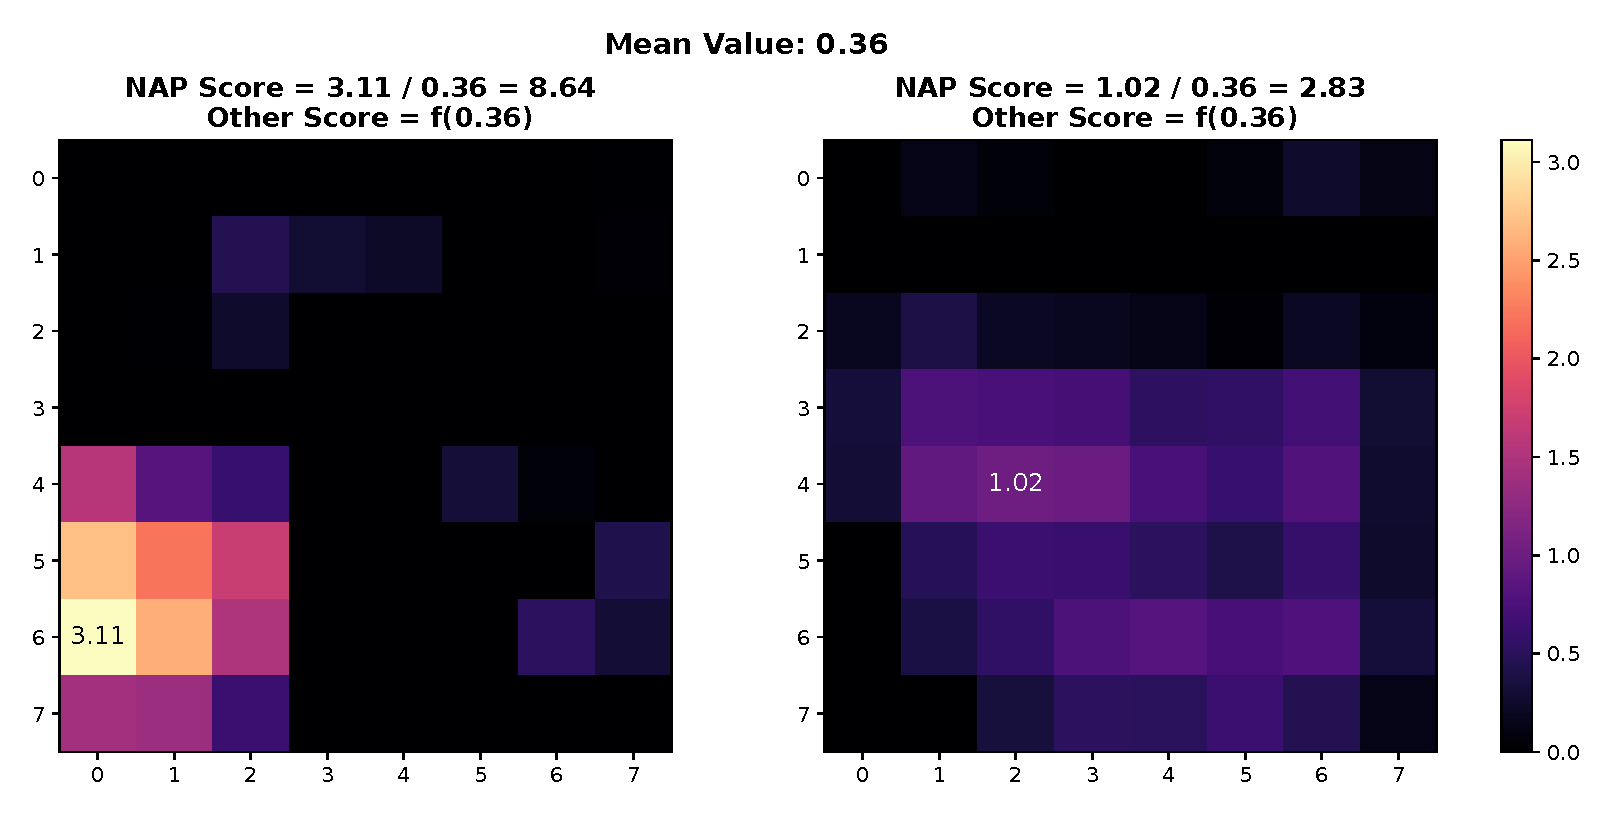
\includegraphics[width=0.49\linewidth]{eps/pair_0_channel_333_vis.eps}
    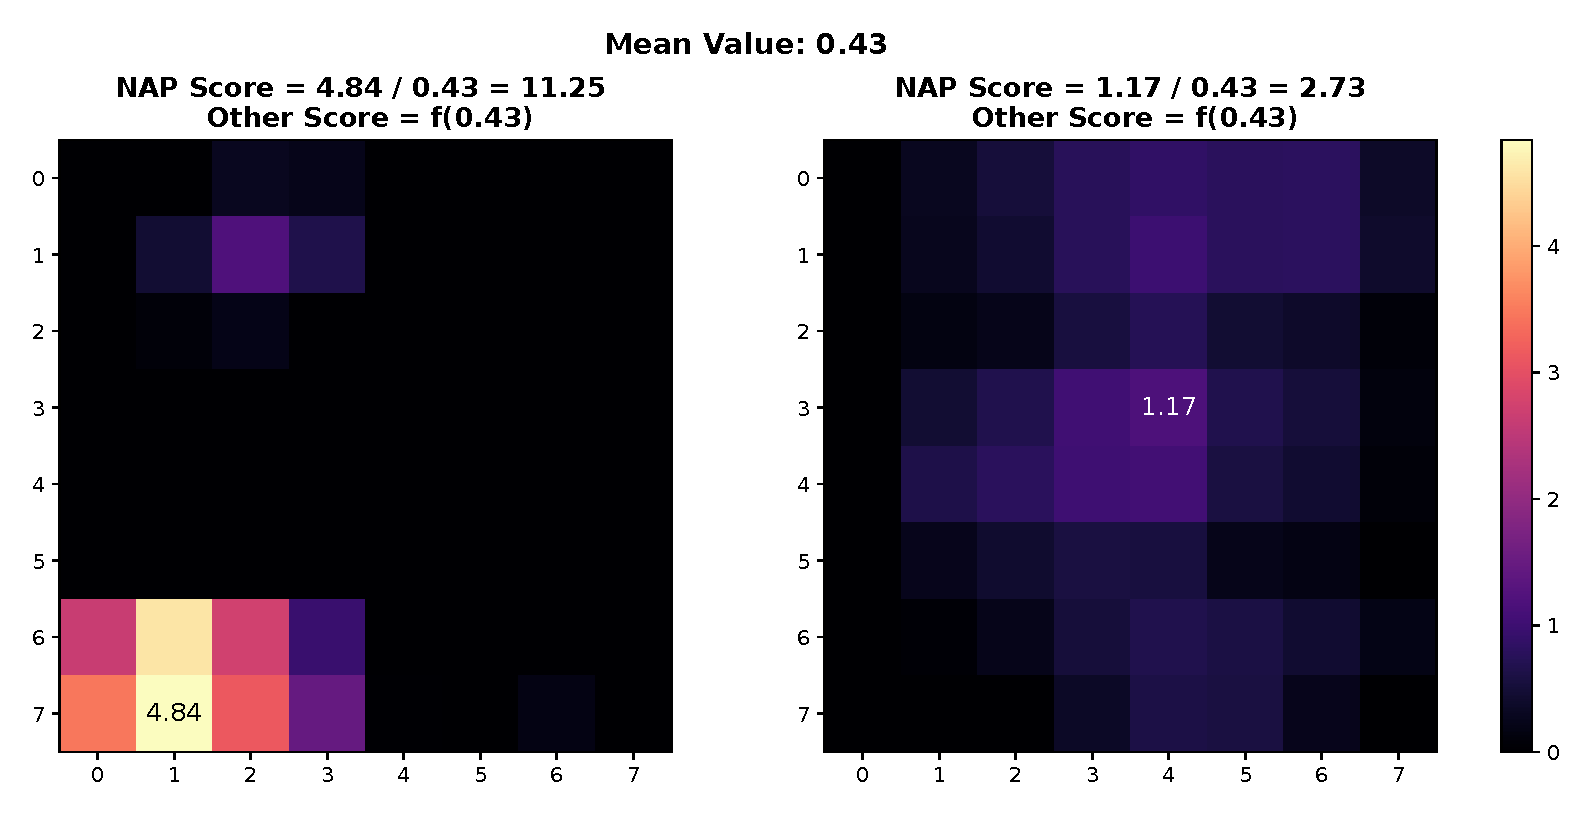
\includegraphics[width=0.49\linewidth]{eps/pair_4_channel_333_vis.eps}
    \label{fig:act_map0}
  \end{subfigure}

  \begin{subfigure}{\linewidth}
    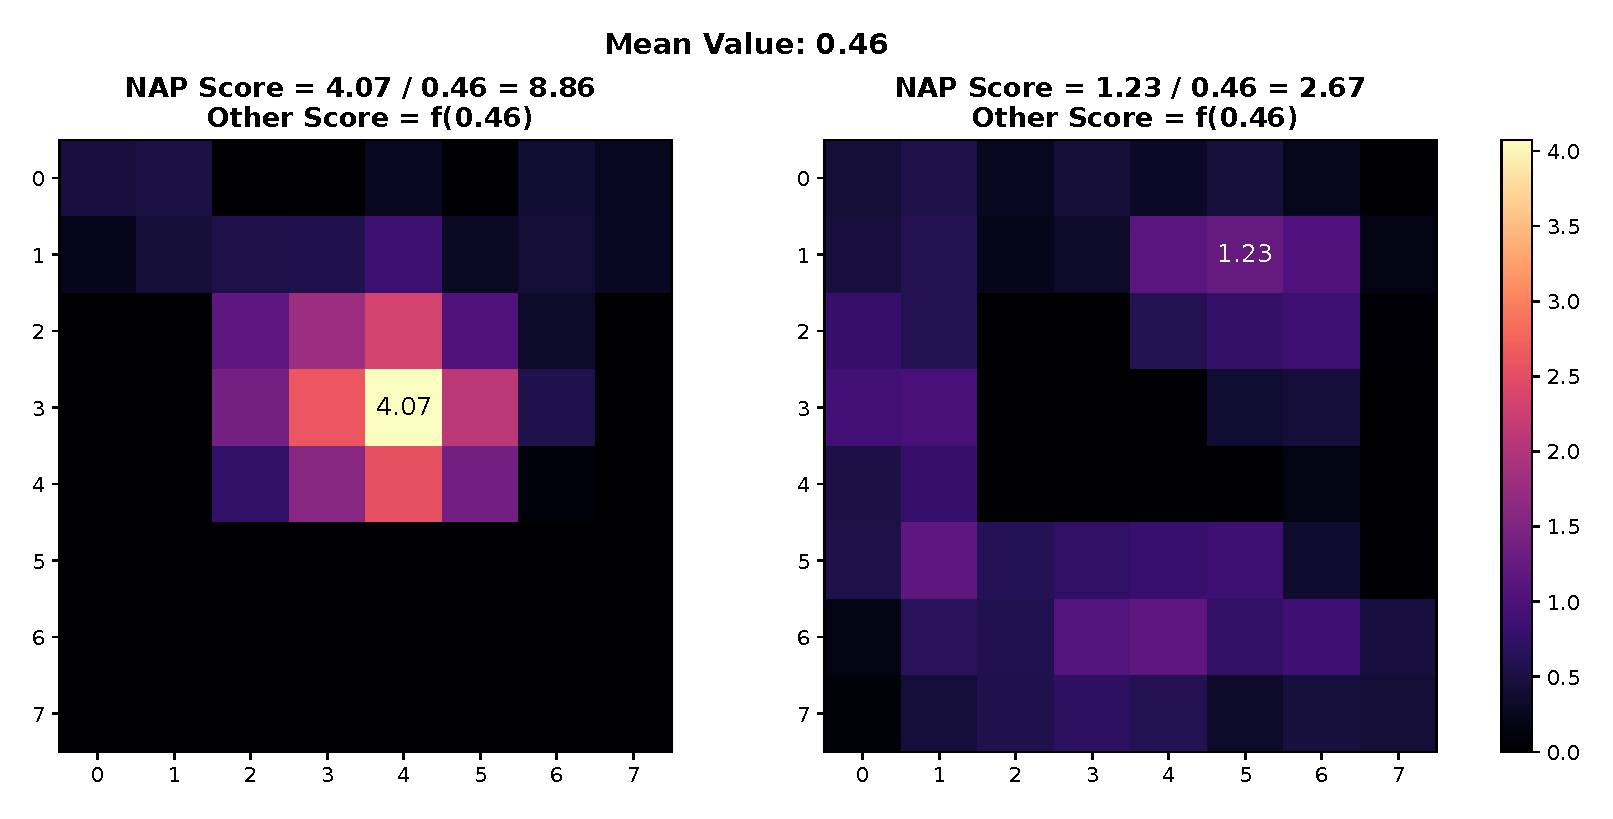
\includegraphics[width=0.49\linewidth]{eps/pair_13_channel_333_vis.eps}
    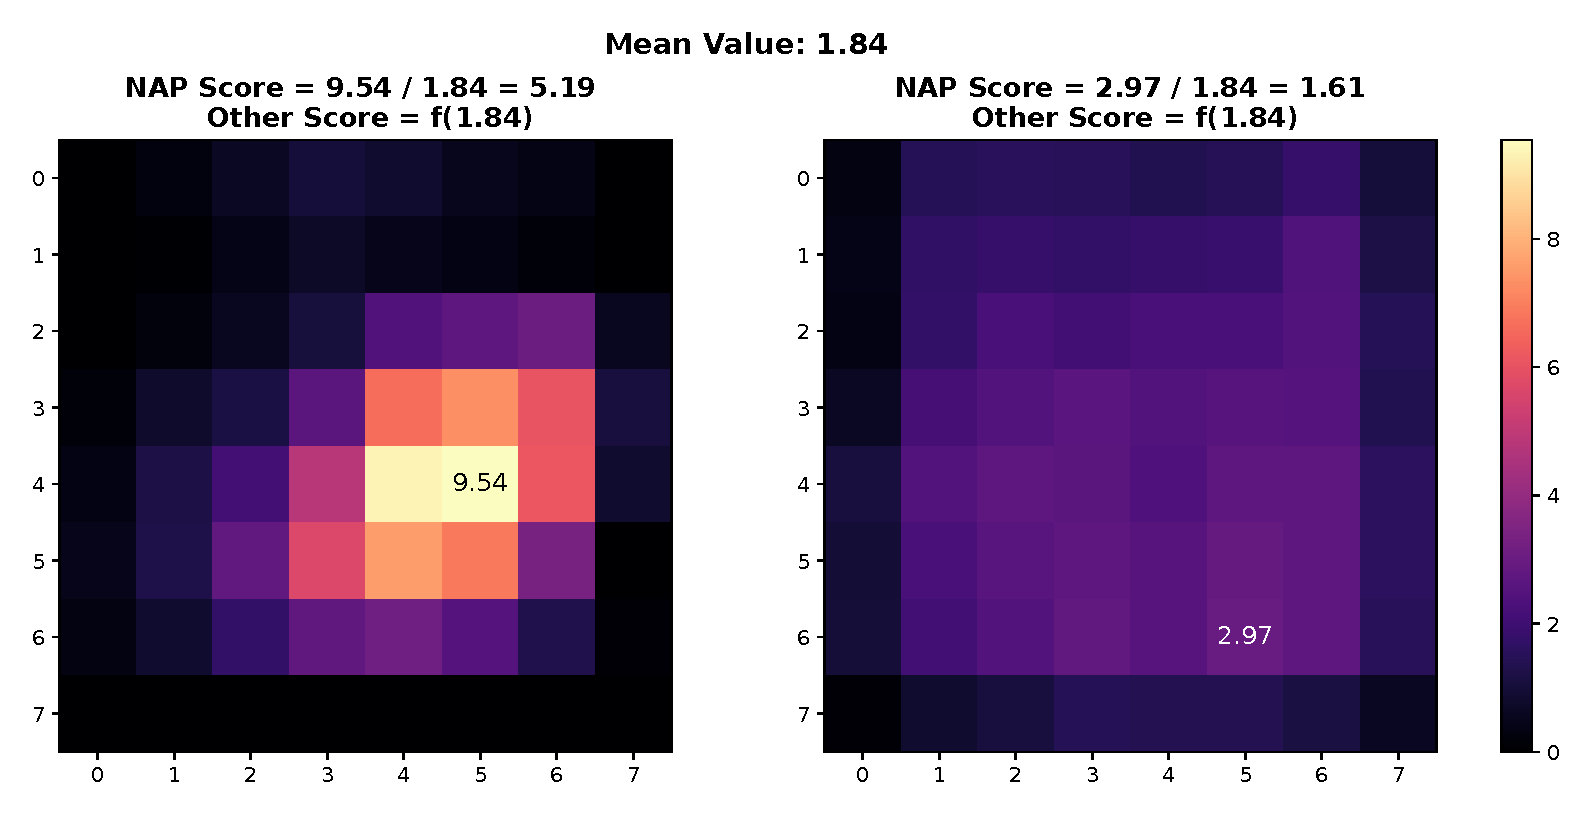
\includegraphics[width=0.49\linewidth]{eps/pair_15_channel_333_vis.eps}
    \label{fig:act_map1}
  \end{subfigure}

  \begin{subfigure}{\linewidth}
    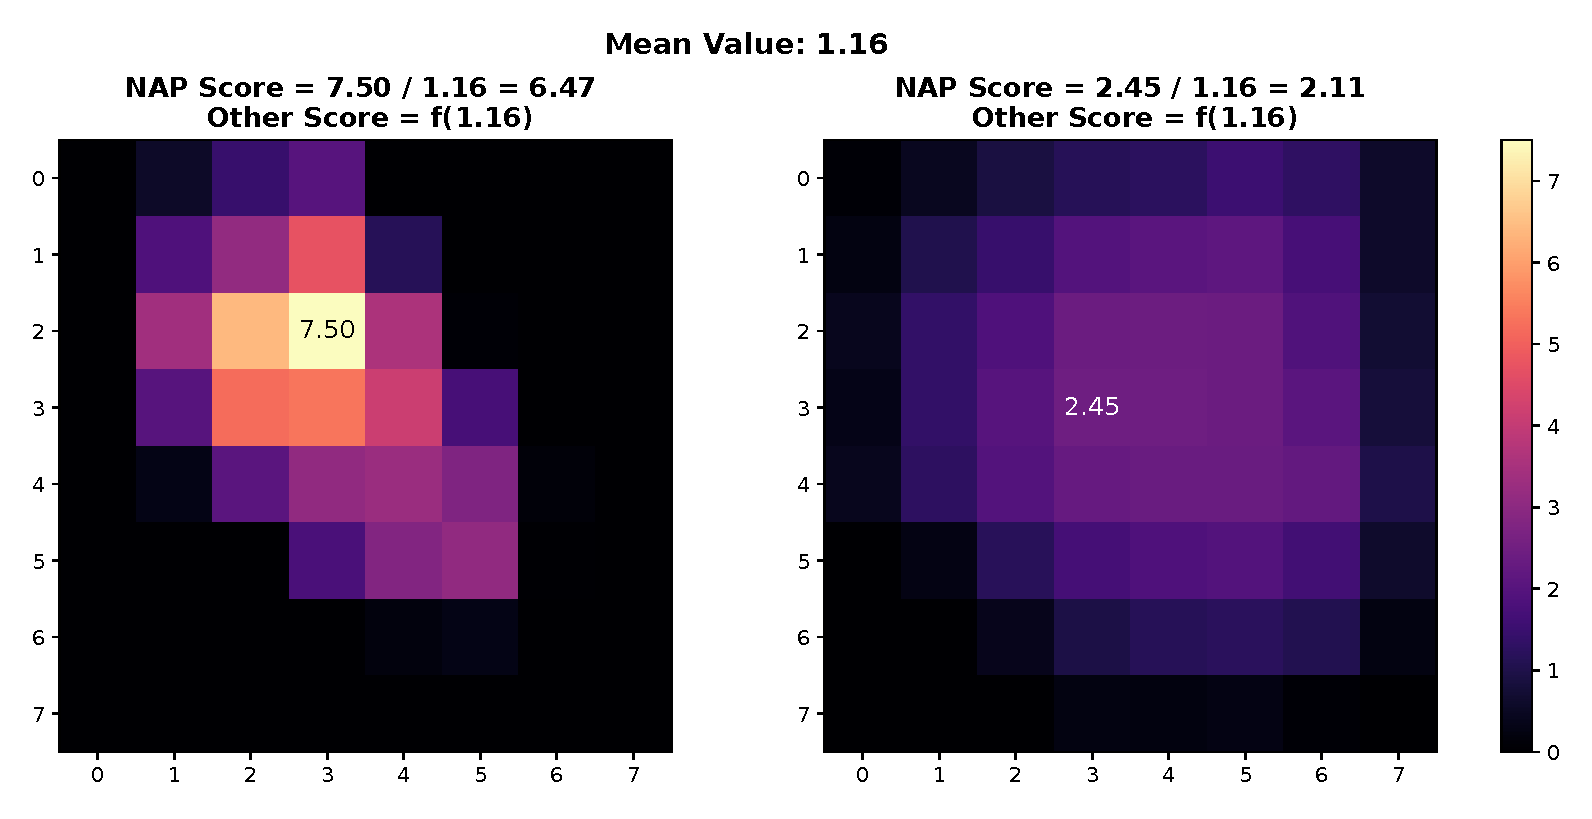
\includegraphics[width=0.49\linewidth]{eps/pair_16_channel_333_vis.eps}
    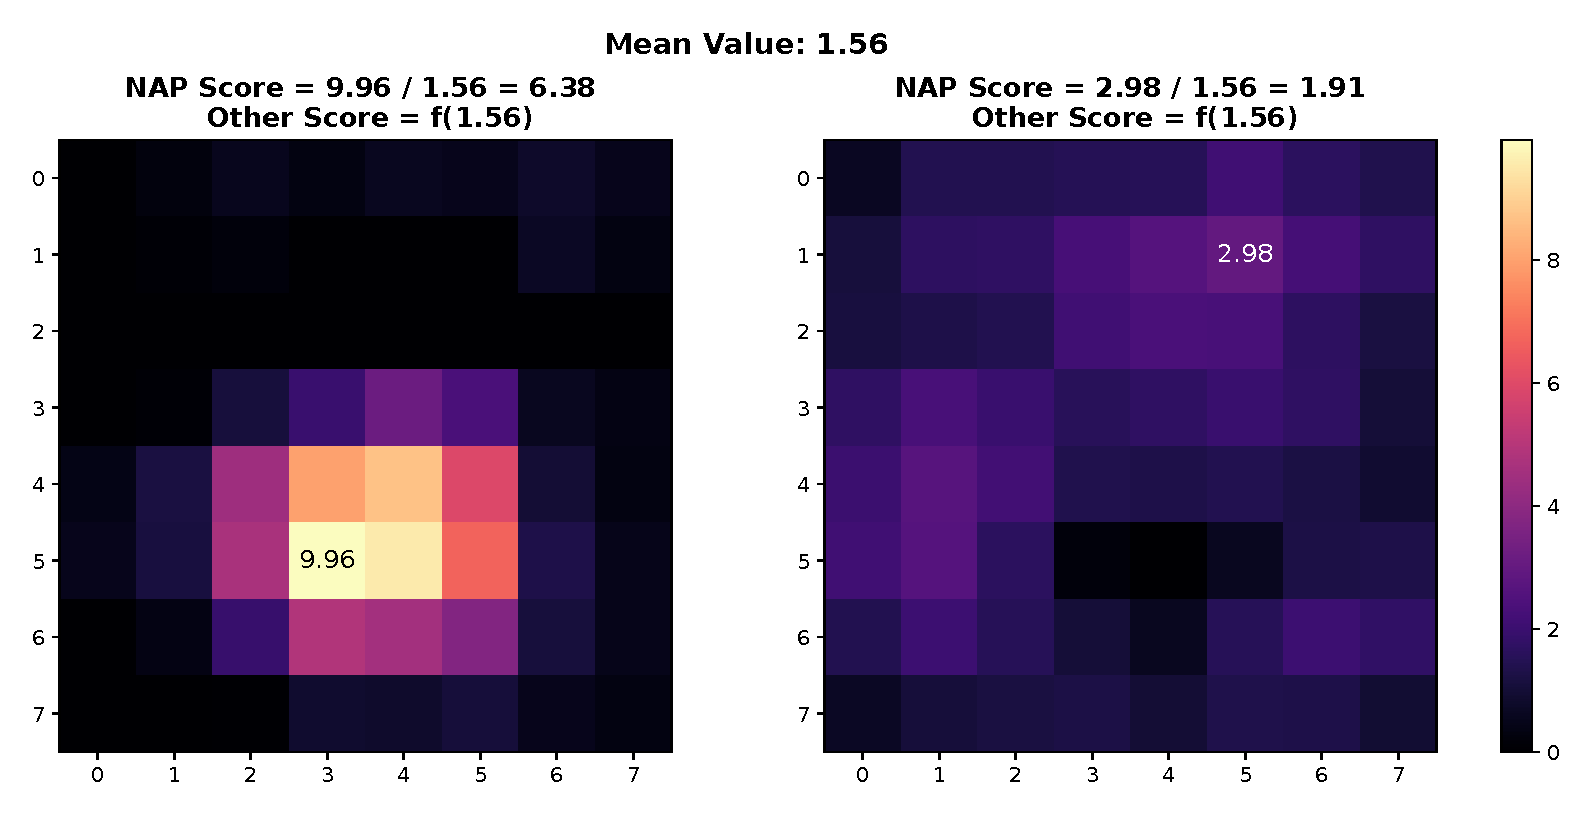
\includegraphics[width=0.49\linewidth]{eps/pair_90_channel_333_vis.eps}
    \label{fig:act_map2}
  \end{subfigure}

  \begin{subfigure}{\linewidth}
    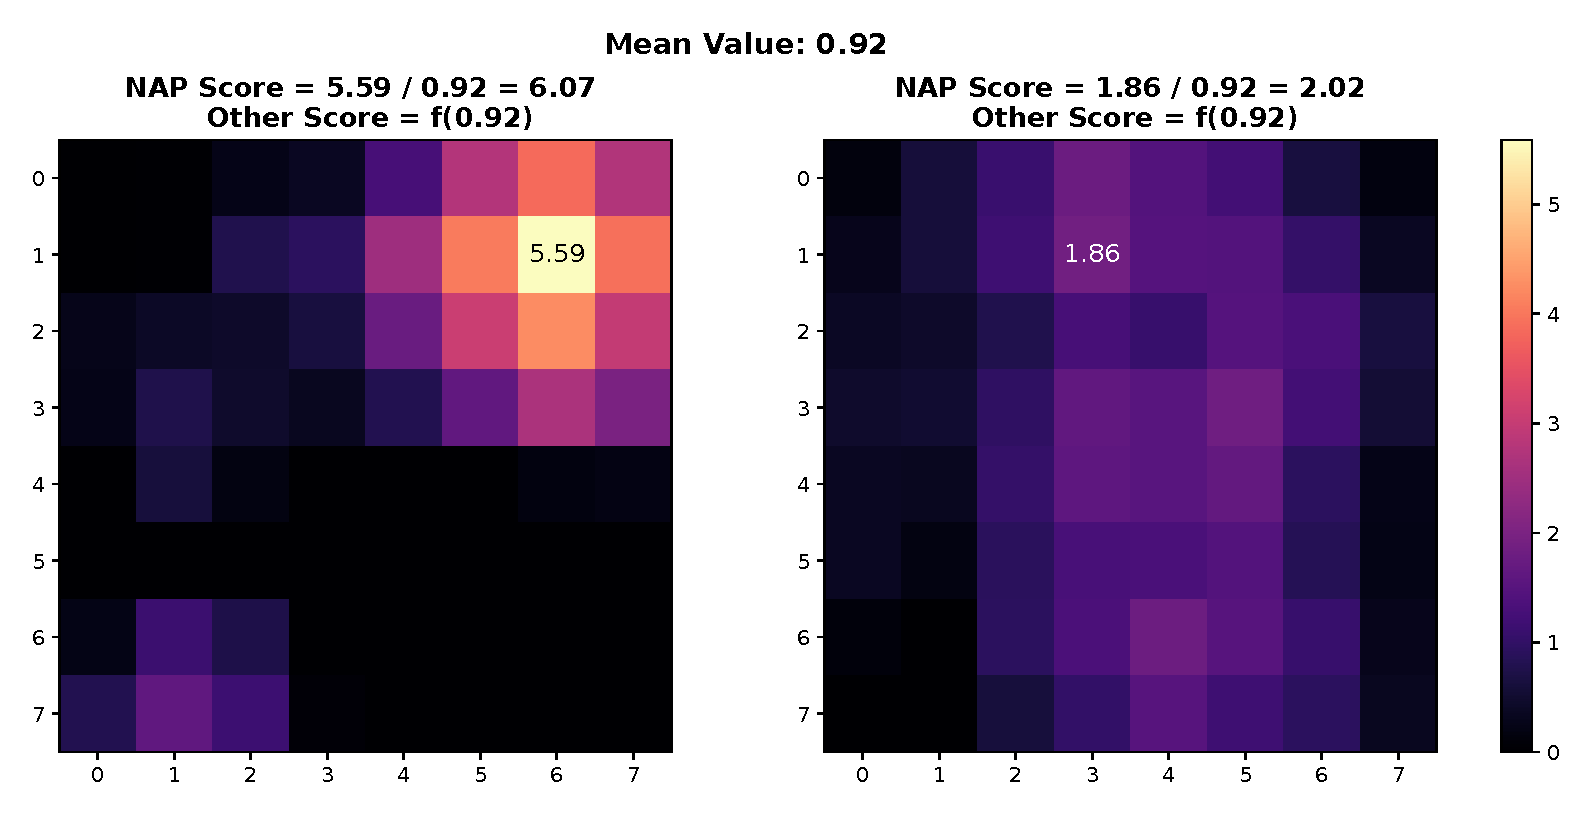
\includegraphics[width=0.49\linewidth]{eps/pair_25_channel_333_vis.eps}
    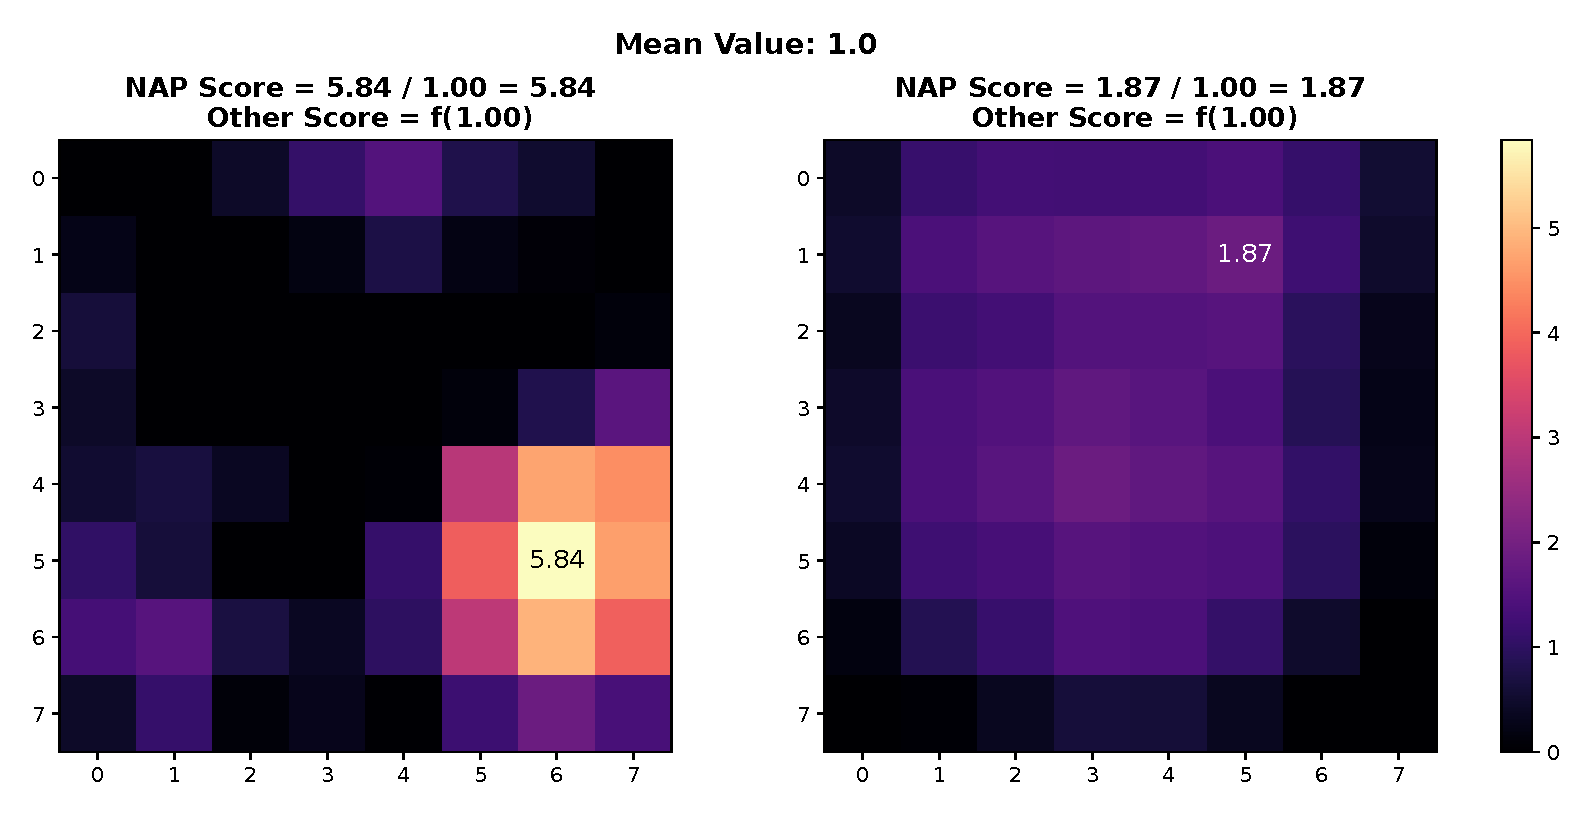
\includegraphics[width=0.49\linewidth]{eps/pair_26_channel_333_vis.eps}
    \label{fig:act_map3}
  \end{subfigure}

  \begin{subfigure}{\linewidth}
    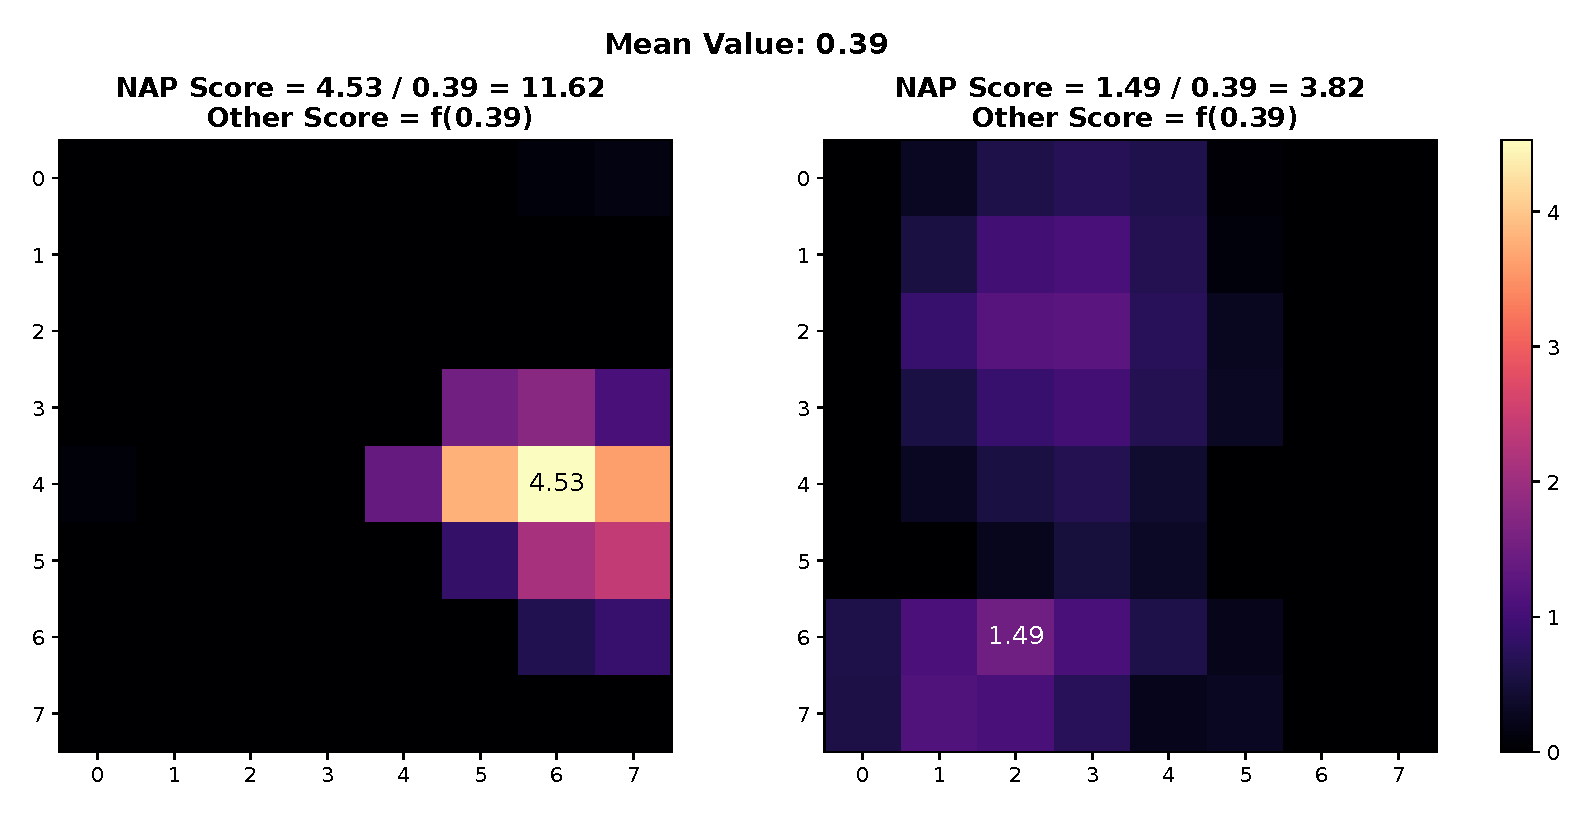
\includegraphics[width=0.49\linewidth]{eps/pair_33_channel_333_vis.eps}
    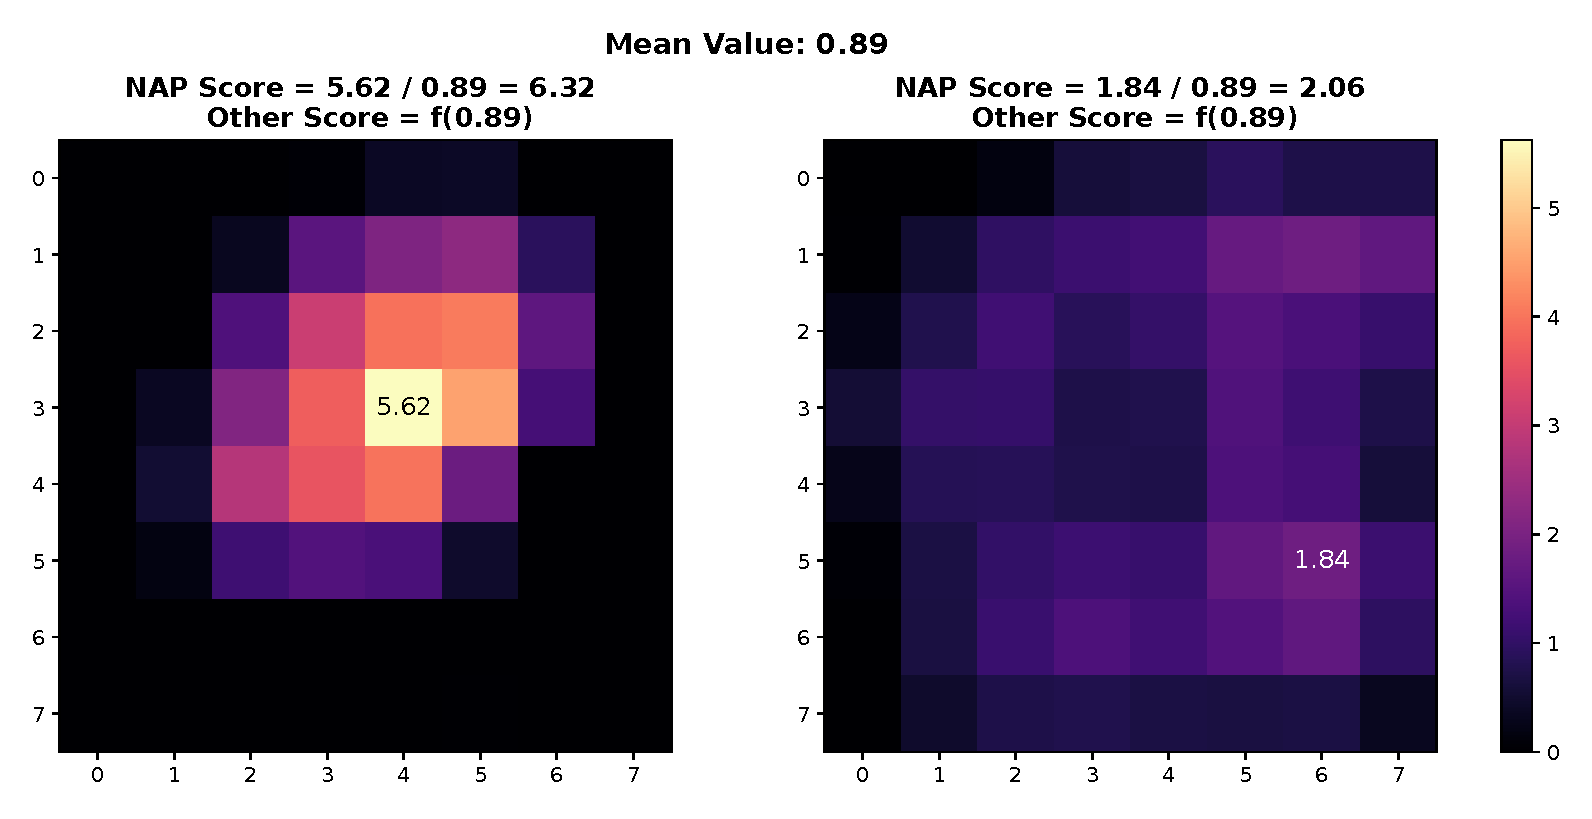
\includegraphics[width=0.49\linewidth]{eps/pair_37_channel_333_vis.eps}
    \label{fig:act_map4}
  \end{subfigure}

  \caption{\textbf{Global pooling disregards the distribution of activation values within channels, making it challenging to differentiate between ID and OOD samples.} Each pair of images in this figure illustrates the activation maps of the penultimate layer for in-distribution (ID) samples (left) and out-of-distribution (OOD) samples (right) within the same channel. In this layer, different channels typically focus on distinct semantic features. When specific features are present in the image, such as certain regions in the left images of each pair, these areas exhibit very high activation values. Although OOD samples lack these specific features, the model's unfamiliarity with OOD data can lead to unpredictable activations, potentially resulting in weak noise activations (right images). This phenomenon is discussed in detail by \cite{sun2021react}. Existing methods often rely on aggregating activation values for OOD detection. Consequently, the average channel activations of ID and OOD samples are not discriminative, making it difficult for existing methods to distinguish between them. However, the NAP score proposed in this paper effectively differentiates them.}
  \label{fig:act_maps0}
\end{figure}
In this section, we present additional examples of activation map visualizations to further illustrate the challenges and phenomena discussed in our work. Specifically, we examine the penultimate layer's activation maps for both in-distribution (ID) and out-of-distribution (OOD) samples. The visualizations provide insights into how global pooling methods can obscure important distinctions between ID and OOD samples by averaging out the spatial distribution of activation values within channels.

As shown in Figure~\ref{fig:act_maps0}, each pair of images displays the activation maps for a given channel. The left image in each pair corresponds to an ID sample, while the right image corresponds to an OOD sample. Different channels in the penultimate layer are typically tuned to capture specific semantic features present in the training data. For ID samples, these features often result in high activation values in particular regions of the activation map. For example, certain regions in the left images of each pair exhibit very high activation values when the corresponding semantic features are present in the ID sample.

In contrast, OOD samples, which do not contain these specific semantic features, may still produce activation responses due to the model's unfamiliarity with such data. This can result in weak noise activations, as observed in the right images of each pair. This phenomenon highlights the difficulty faced by traditional OOD detection methods that rely on aggregated activation values, as discussed by \cite{sun2021react}. These methods often fail to differentiate between ID and OOD samples because the average channel activations do not provide sufficient discriminative power.

However, the NAP score proposed in this paper addresses this issue by effectively distinguishing between ID and OOD samples based on a more nuanced analysis of activation patterns. The following visualizations exemplify the described behavior and underscore the importance of considering the distribution of activation values within channels for robust OOD detection.
%%%%%%%%%%%%%%%%%%%%%%%%%%%%%%%%%%%%%%%%%%%%%%%%%%%%%%%%%%%%%%%%%%%%%%%%%%%
\section{Limitations}
\label{appendix:limit}
The proposed method relies on the neural network's ability to effectively learn specific semantic features of the ID dataset in the penultimate layer, and the assumption that OOD samples do not possess these features. If OOD samples exhibit similar semantic features or if the neural network is not well-trained, the effectiveness of the proposed method may be compromised.
%%%%%%%%%%%%%%%%%%%%%%%%%%%%%%%%%%%%%%%%%%%%%%%%%%%%%%%%%%%%%%%%%%%%%%%%%%%

\begin{figure}[!h]
  \centering
  \begin{subfigure}{\linewidth}
    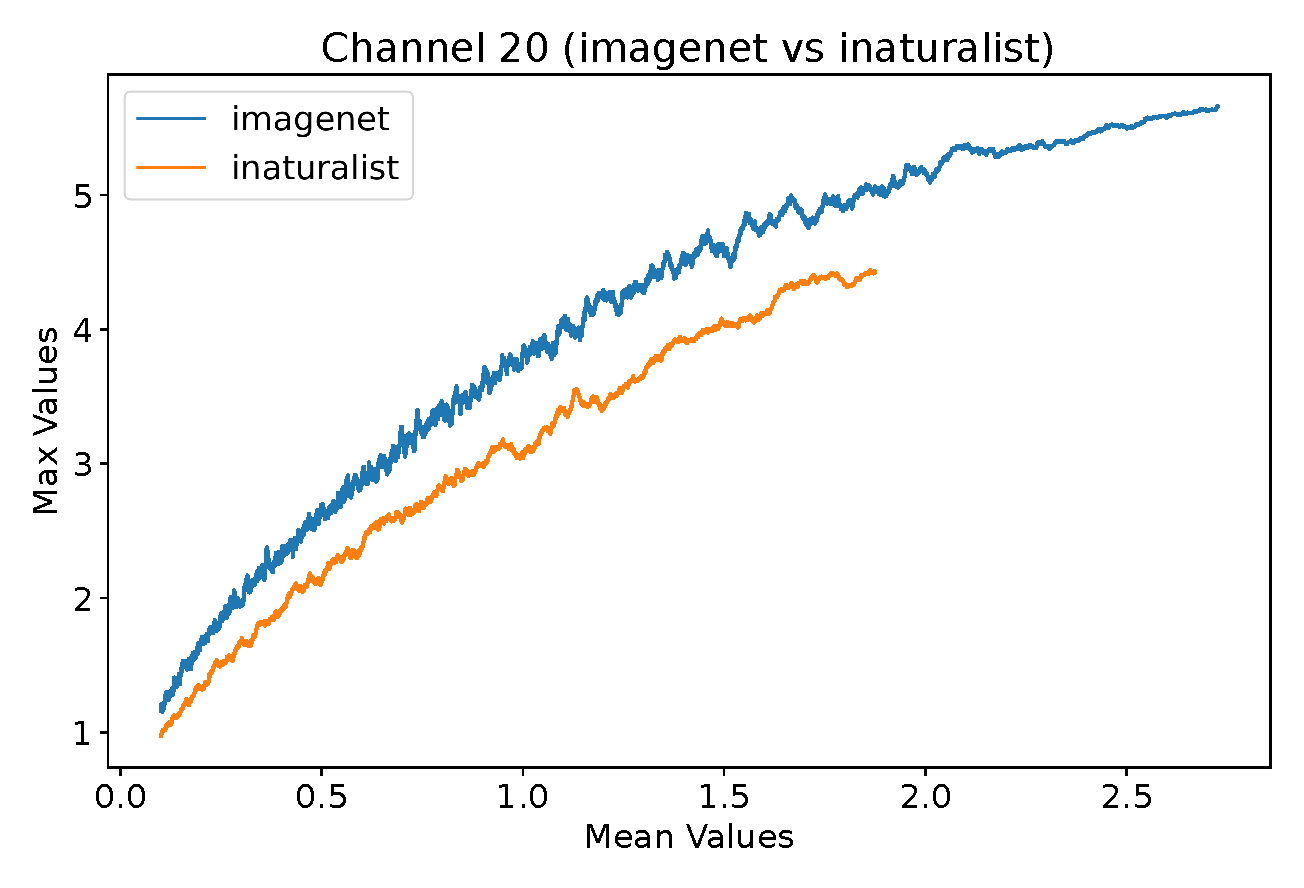
\includegraphics[width=0.24\linewidth]{eps/ap_mo_channel_20.eps}
    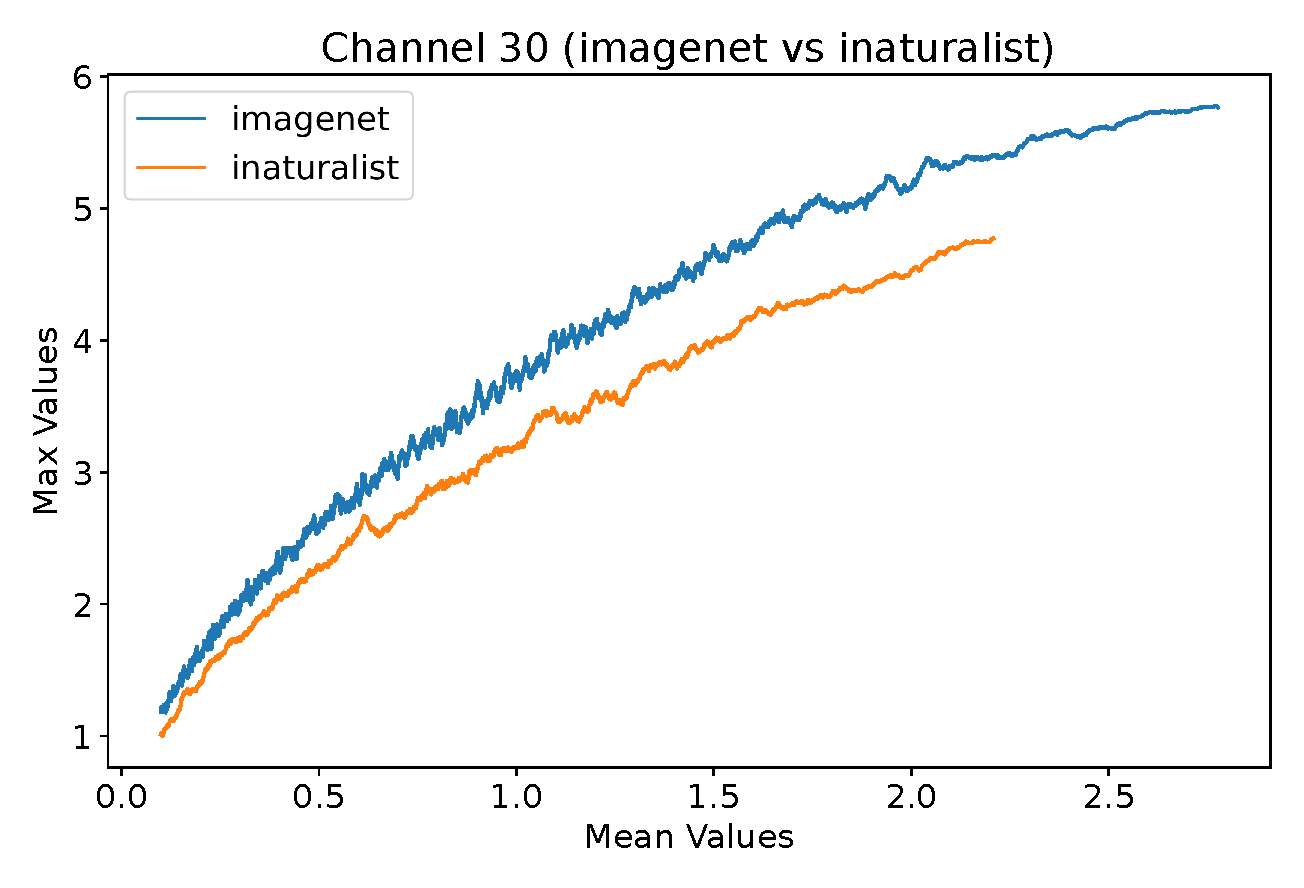
\includegraphics[width=0.24\linewidth]{eps/ap_mo_channel_30.eps}
    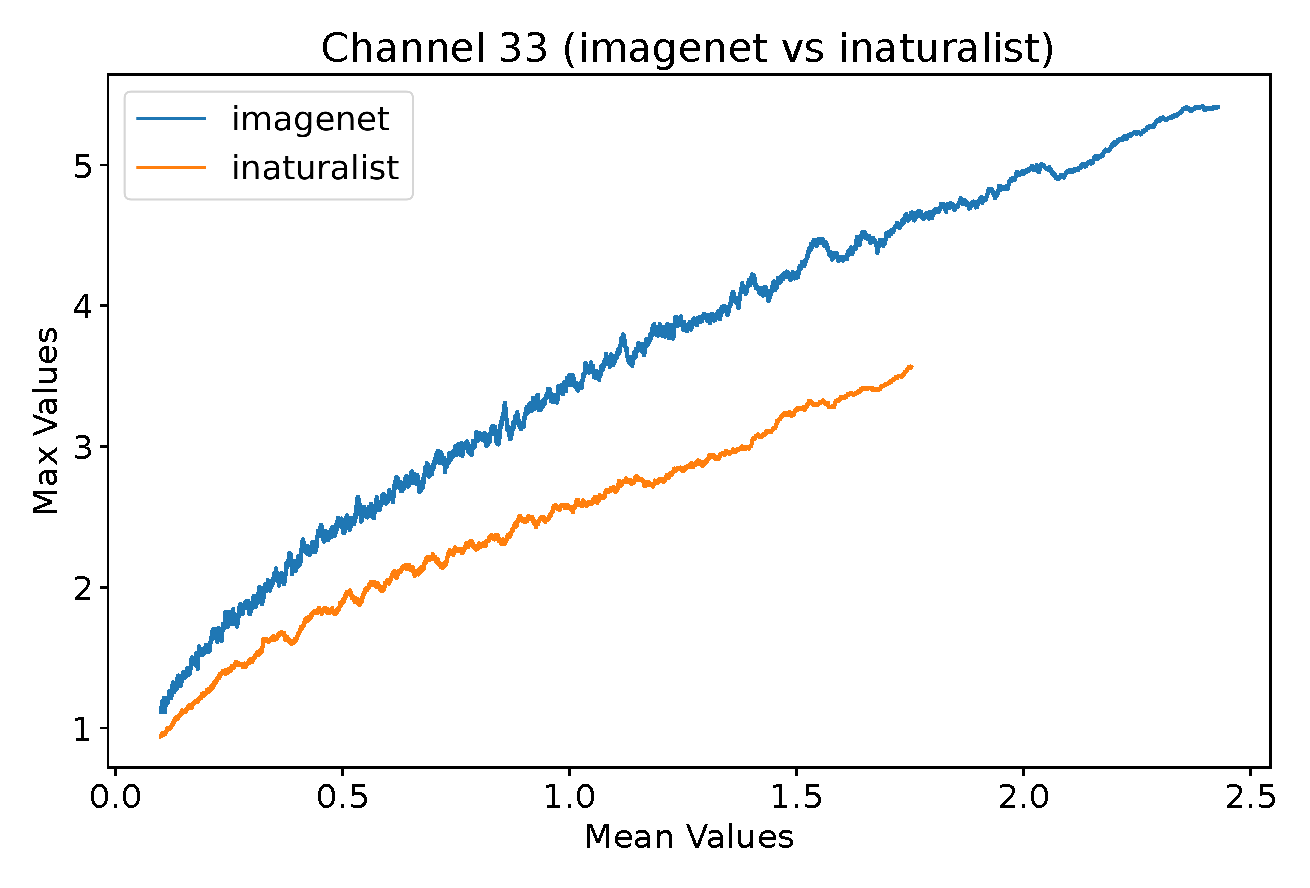
\includegraphics[width=0.24\linewidth]{eps/ap_mo_channel_33.eps}
    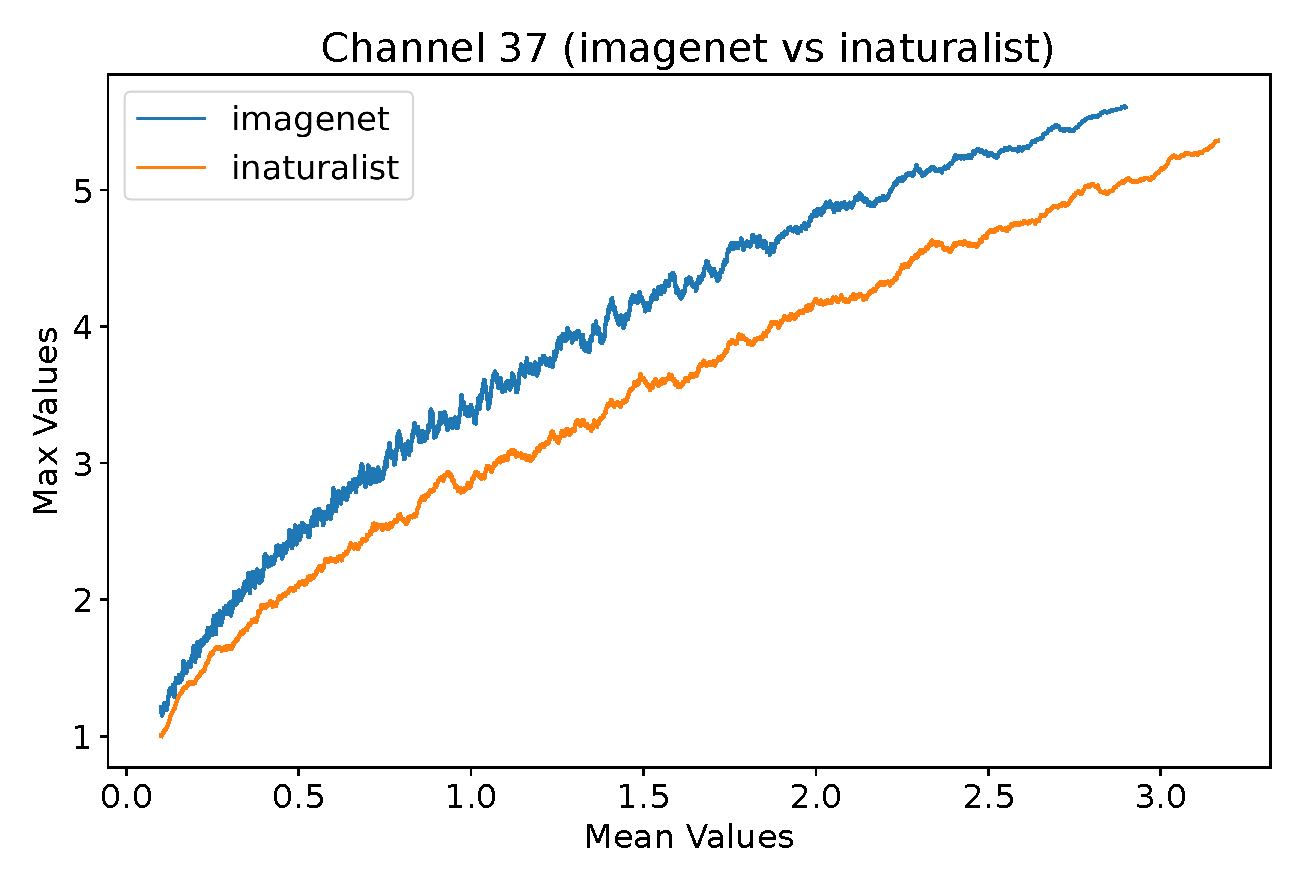
\includegraphics[width=0.24\linewidth]{eps/ap_mo_channel_37.eps}
    \label{fig:mobilenet-r1}
  \end{subfigure}

  \begin{subfigure}{\linewidth}
    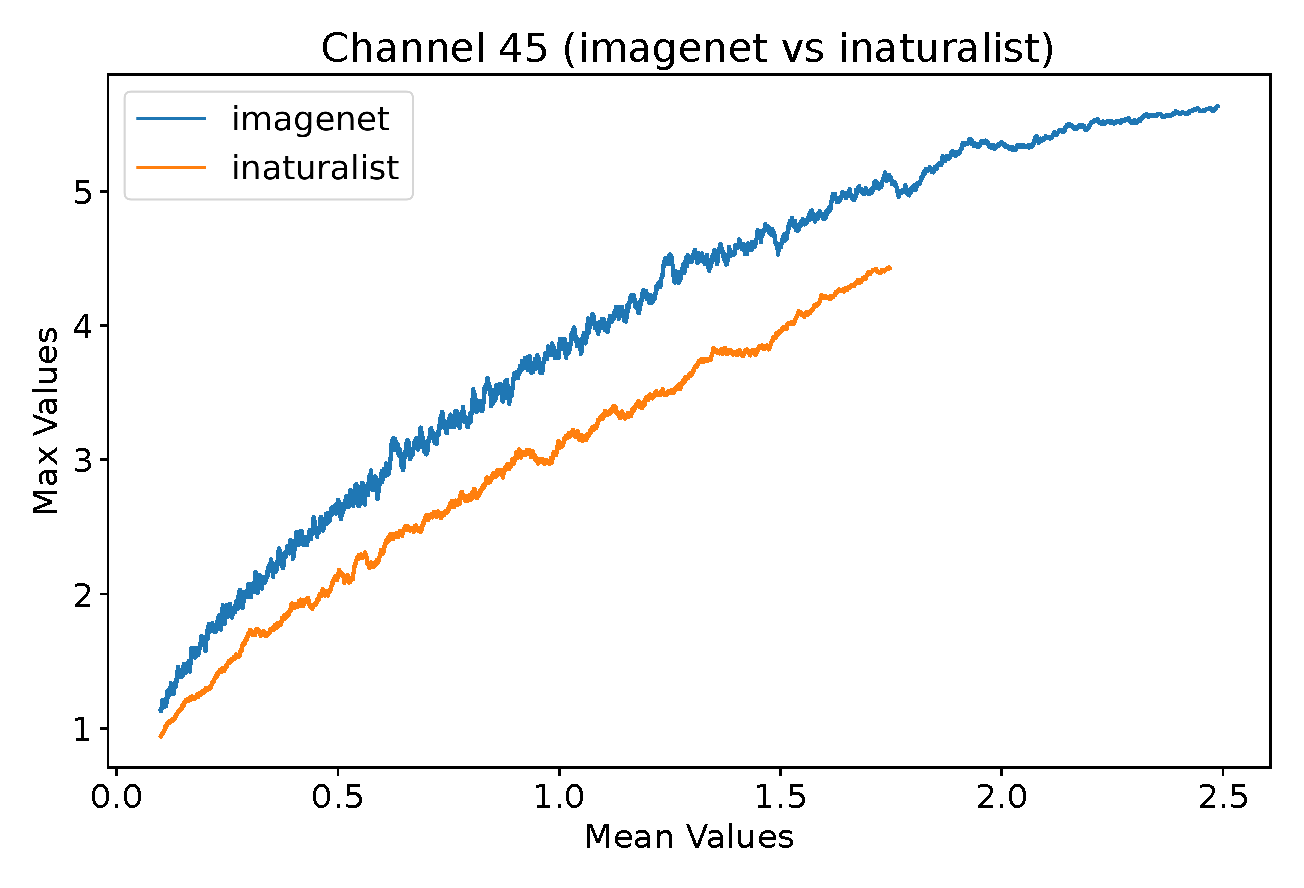
\includegraphics[width=0.24\linewidth]{eps/ap_mo_channel_45.eps}
    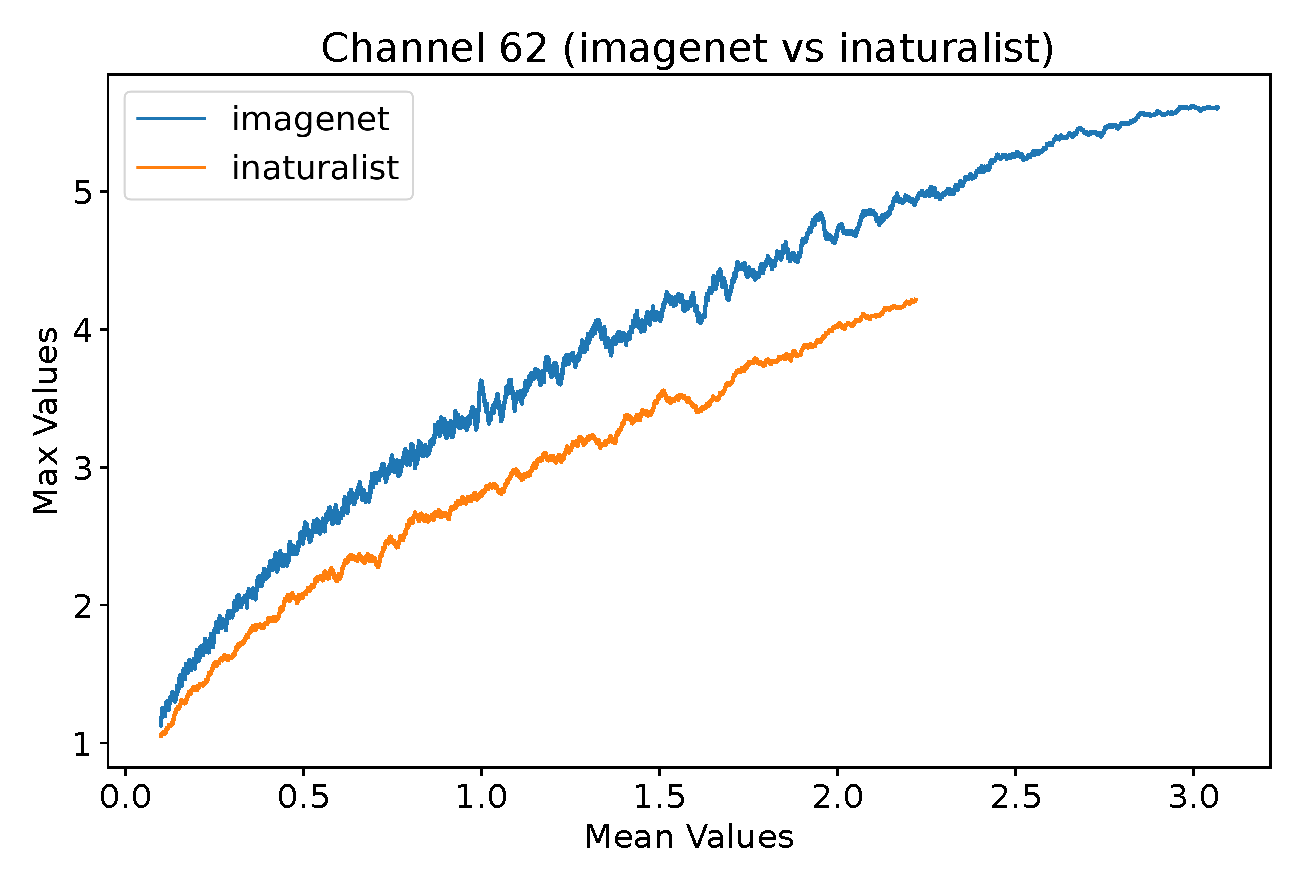
\includegraphics[width=0.24\linewidth]{eps/ap_mo_channel_62.eps}
    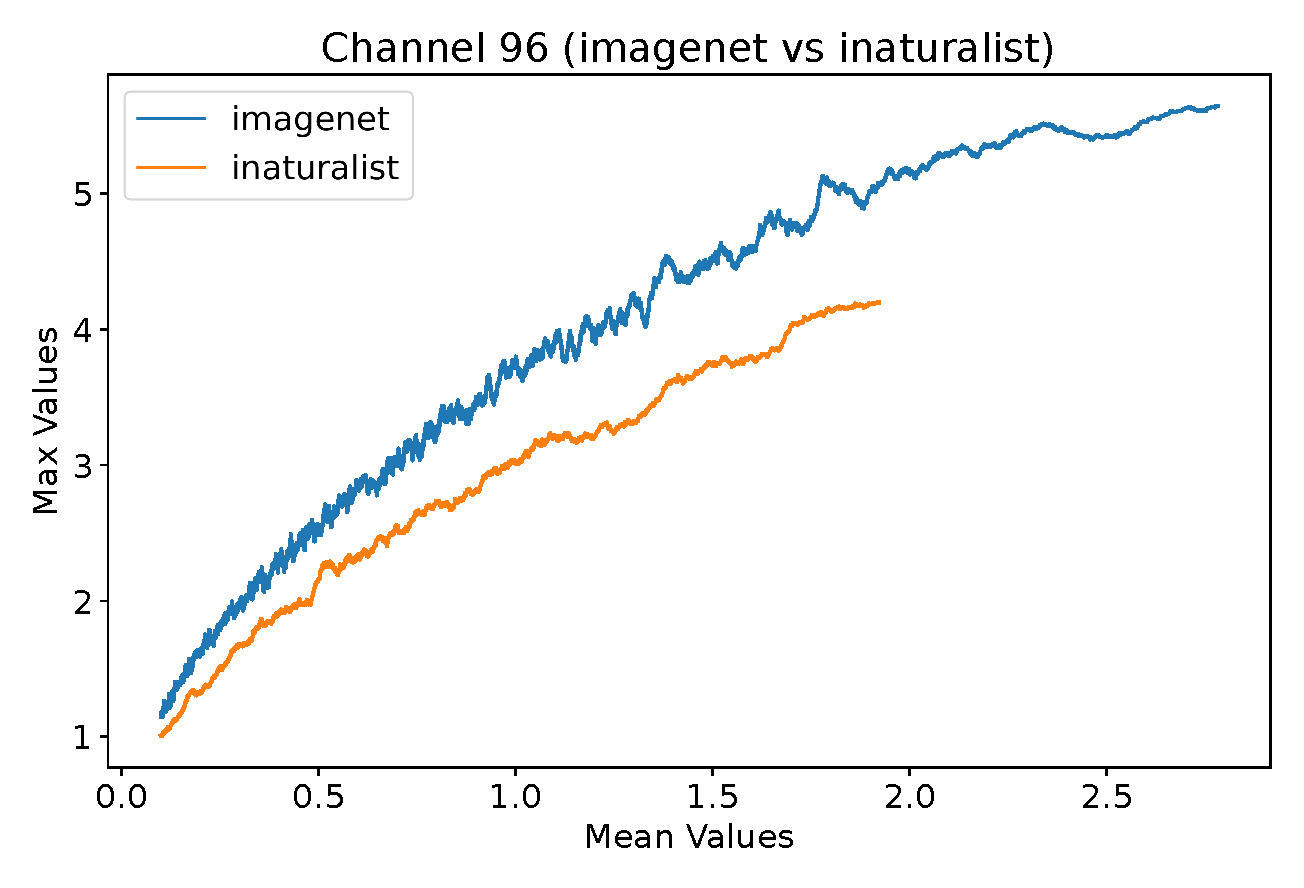
\includegraphics[width=0.24\linewidth]{eps/ap_mo_channel_96.eps}
    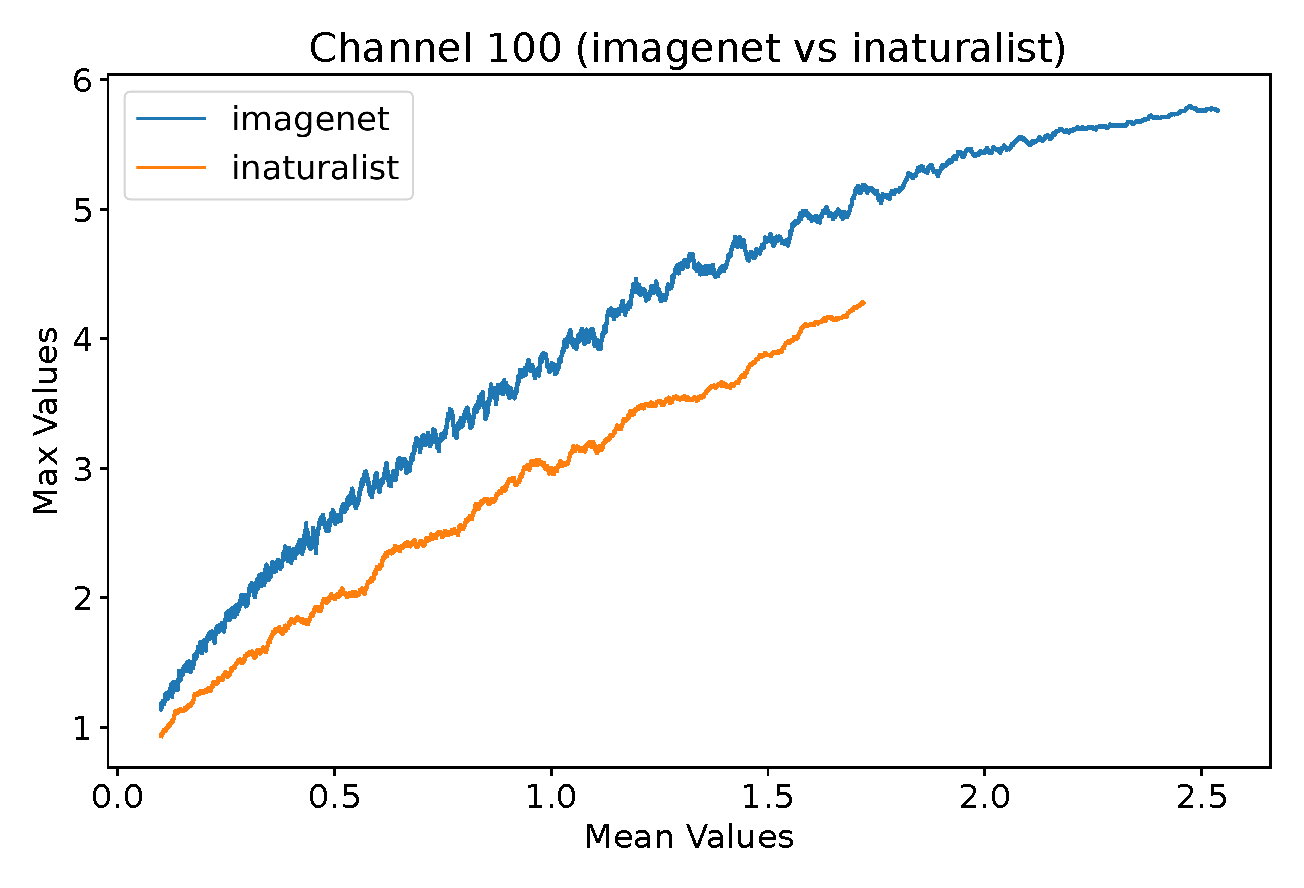
\includegraphics[width=0.24\linewidth]{eps/ap_mo_channel_100.eps}
    \label{fig:mobilenet-r2}
  \end{subfigure}

  \caption{\textbf{Activation distribution at penultimate layer before global pooling operation within the MobileNetV2 architecture~\cite{sandler2018mobilenetv2} applied to ImageNet-1k and iNaturalist datasets~\cite{van2018inaturalist}.} We only include data points with an average activation over $0.1$. The figures show that our Neural Activation Prior (NAP) method is also effective in MobileNetV2, proving that NAP can be applied to different architectures.}
  \label{fig:appendix-e-mobilenet}
\end{figure}

\begin{figure}[!h]
  \centering
  \begin{subfigure}{\linewidth}
  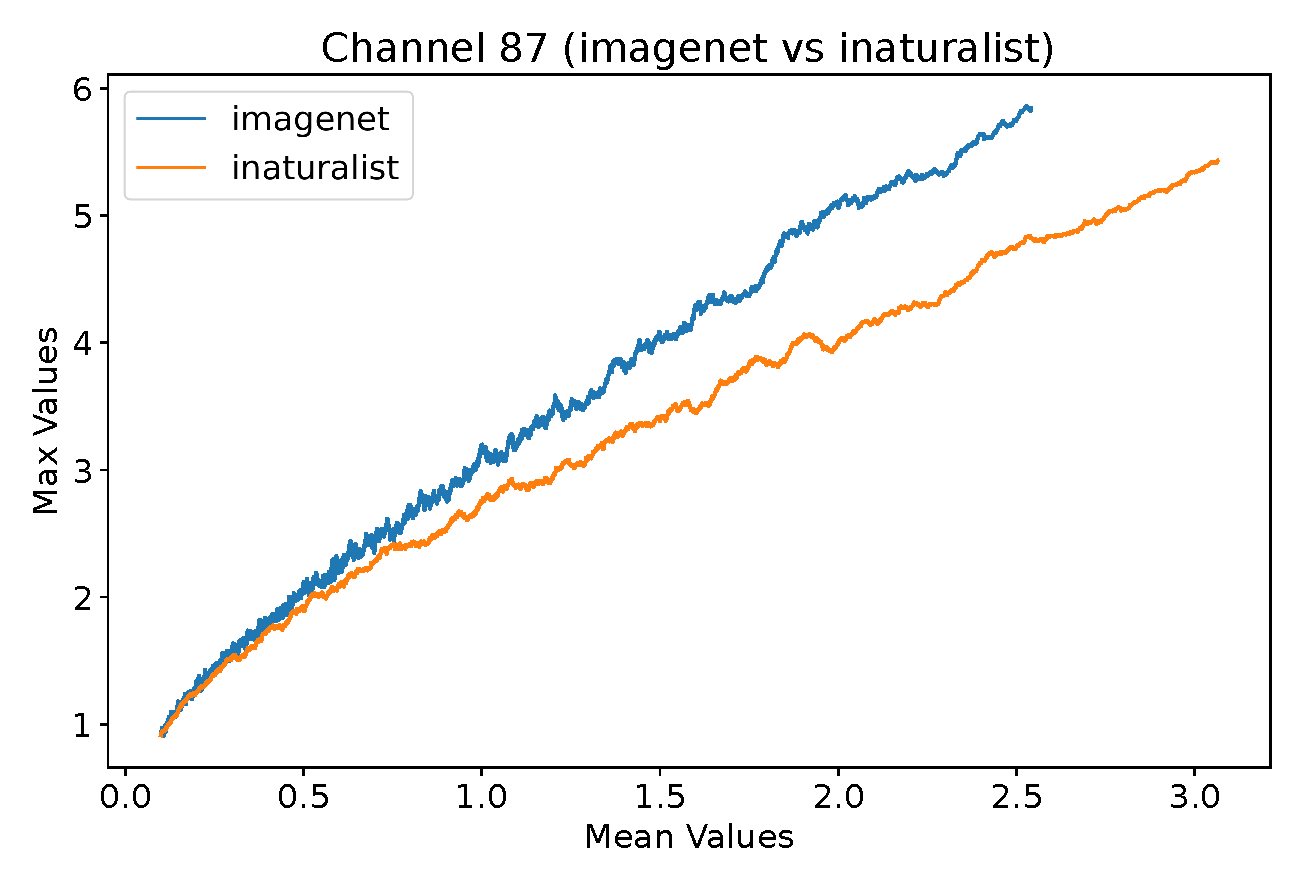
\includegraphics[width=0.24\linewidth]{eps/ap_re_channel_87.eps}
    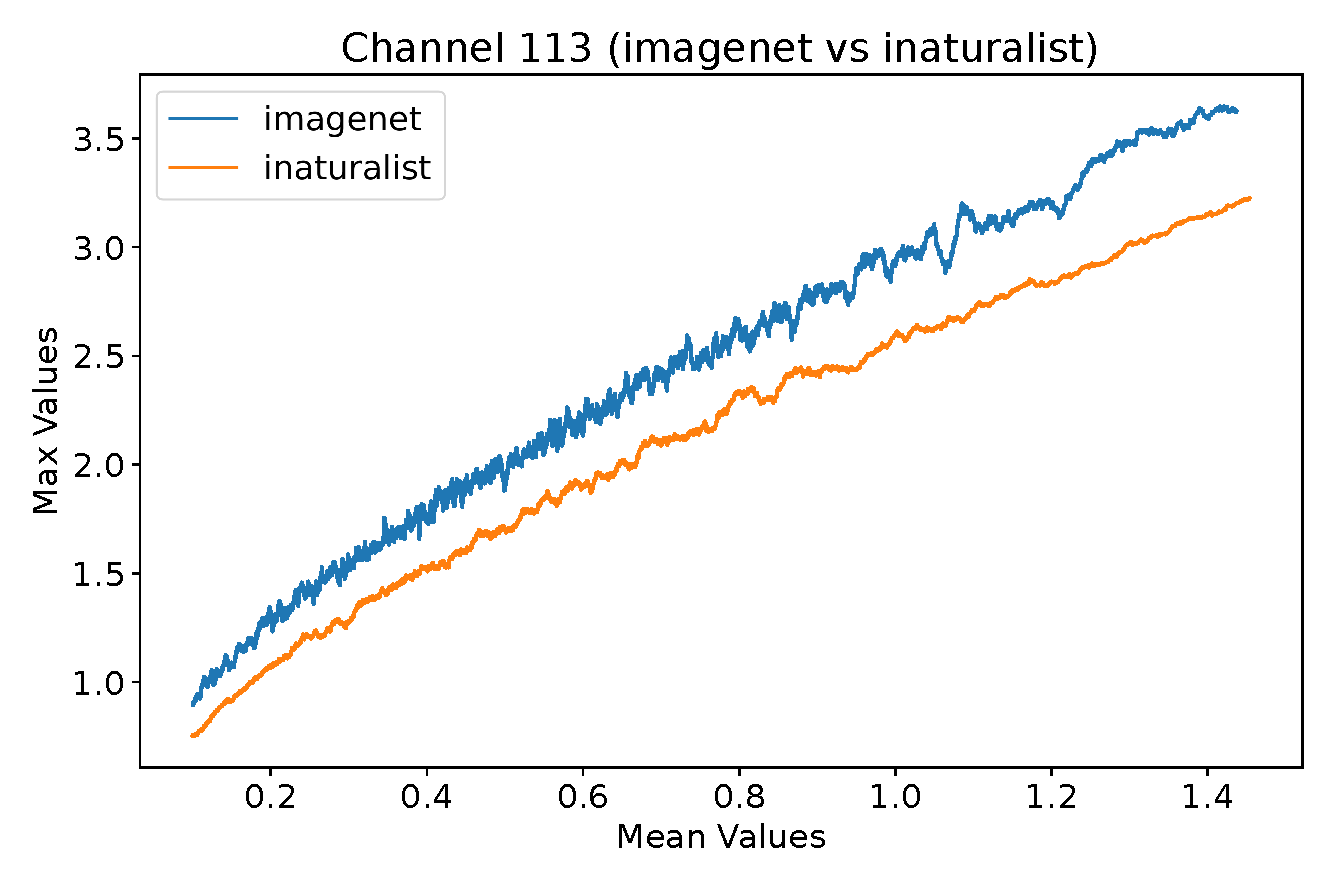
\includegraphics[width=0.24\linewidth]{eps/ap_re_channel_113.eps}
    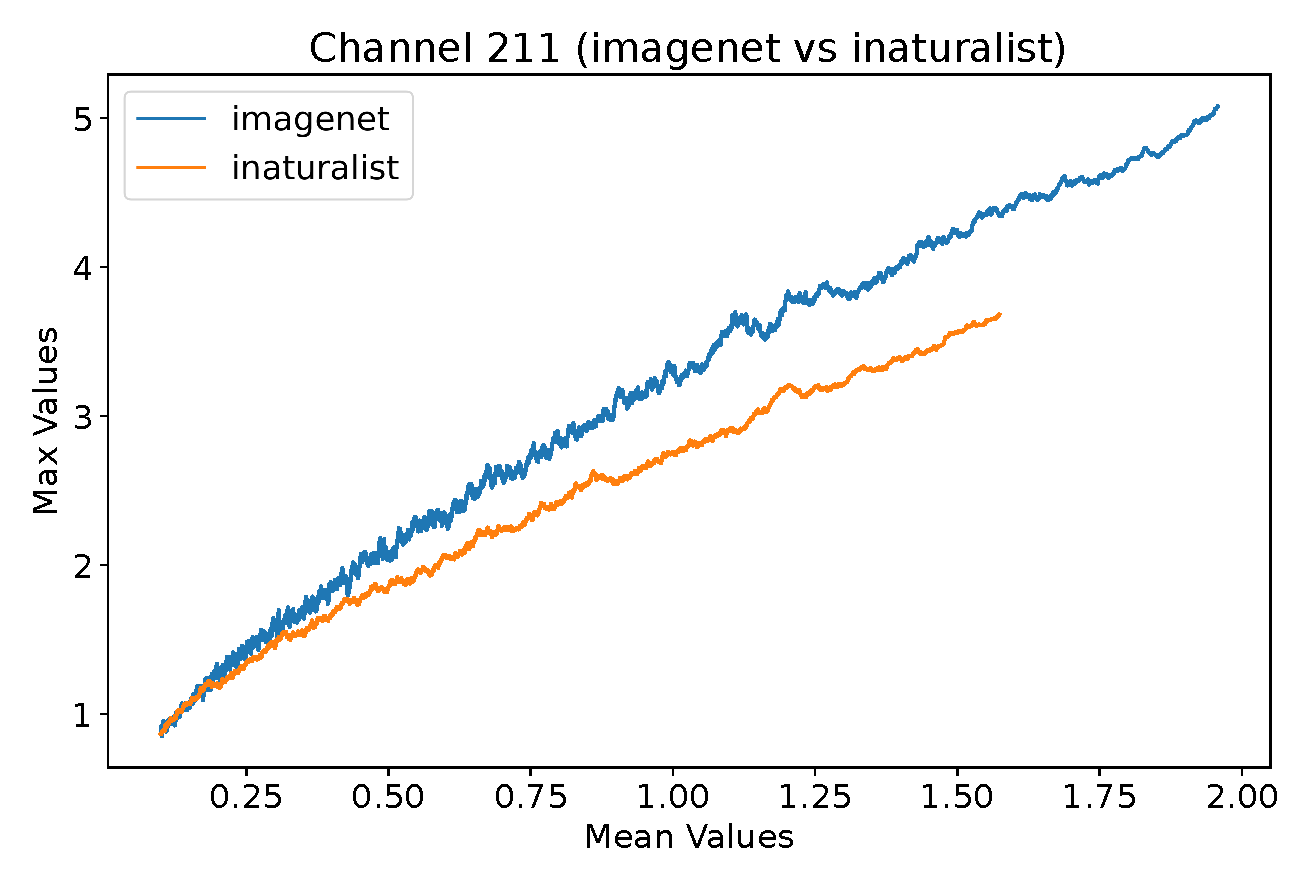
\includegraphics[width=0.24\linewidth]{eps/ap_re_channel_211.eps}
    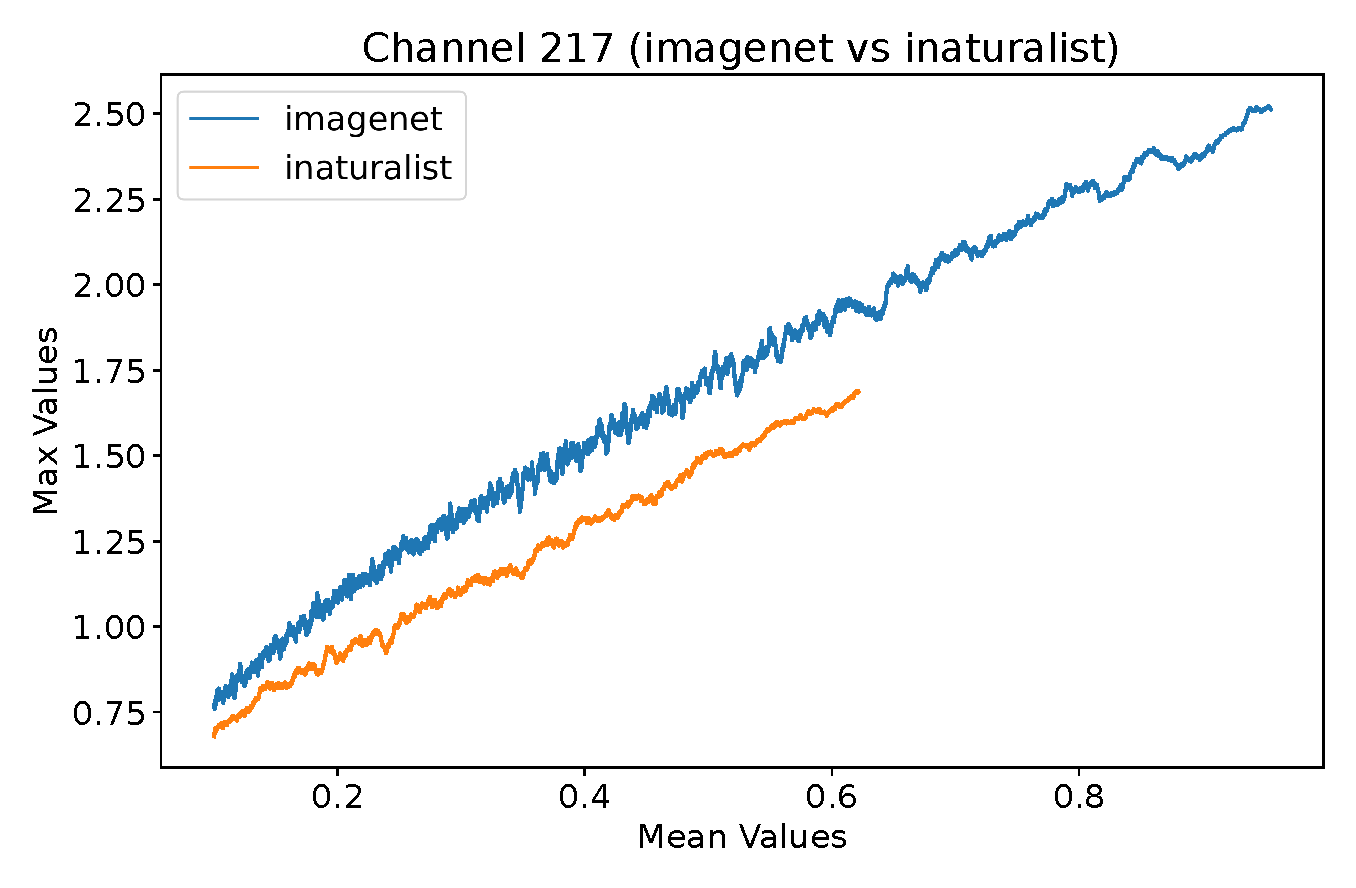
\includegraphics[width=0.24\linewidth]{eps/ap_re_channel_217.eps}
    \label{fig:resnet-r1}
  \end{subfigure}

  \begin{subfigure}{\linewidth}
    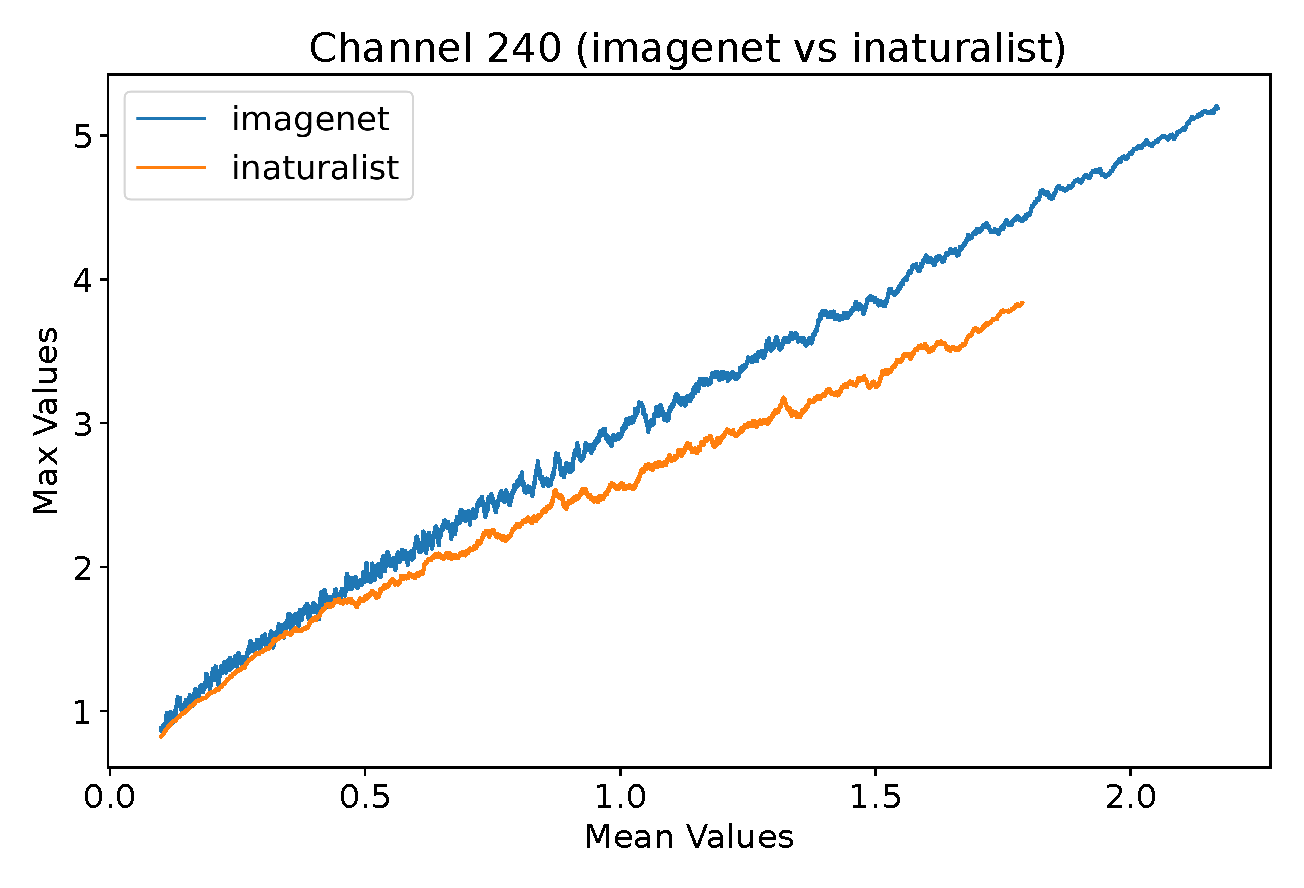
\includegraphics[width=0.24\linewidth]{eps/ap_re_channel_240.eps}
    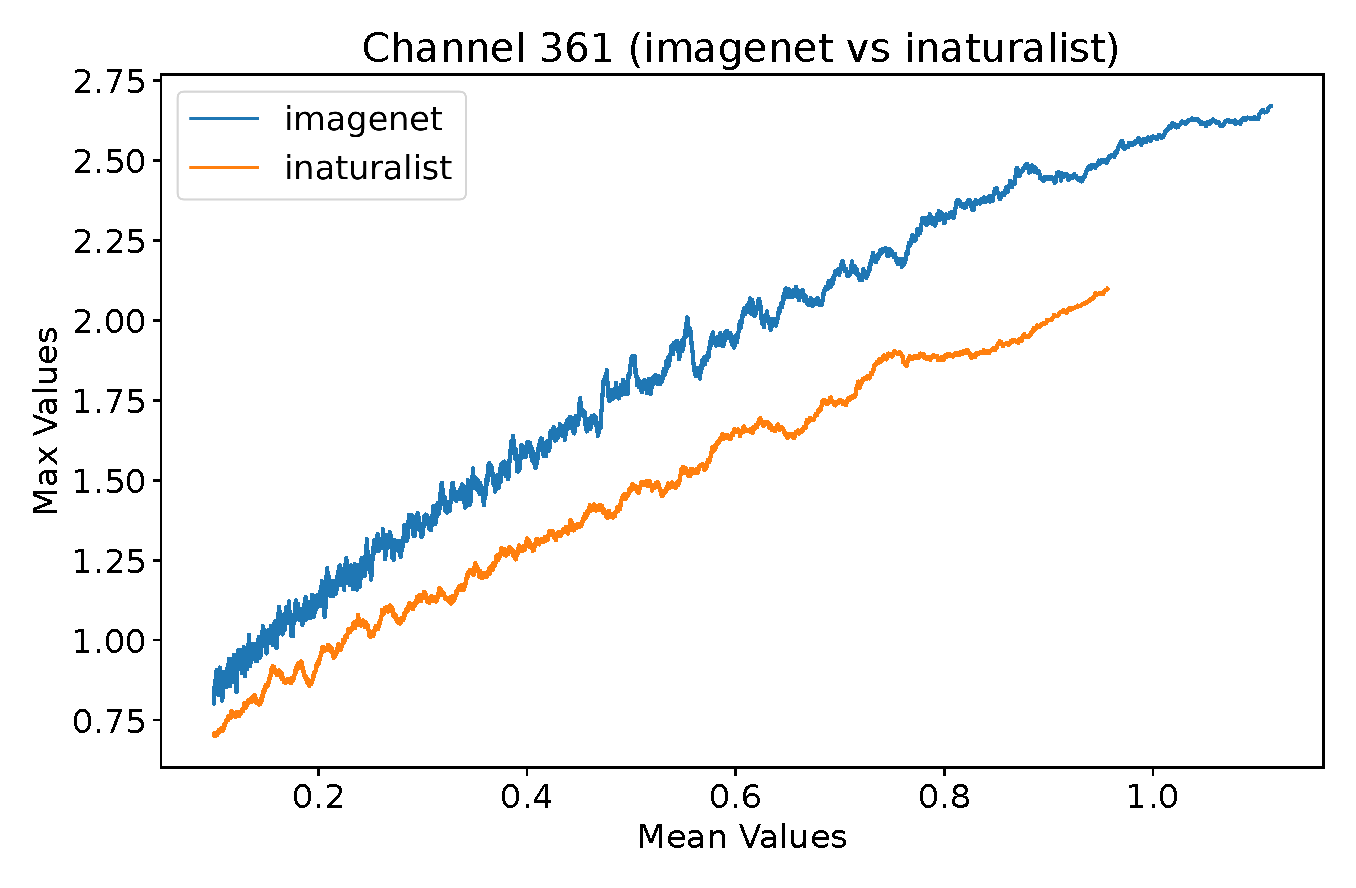
\includegraphics[width=0.24\linewidth]{eps/ap_re_channel_361.eps}
    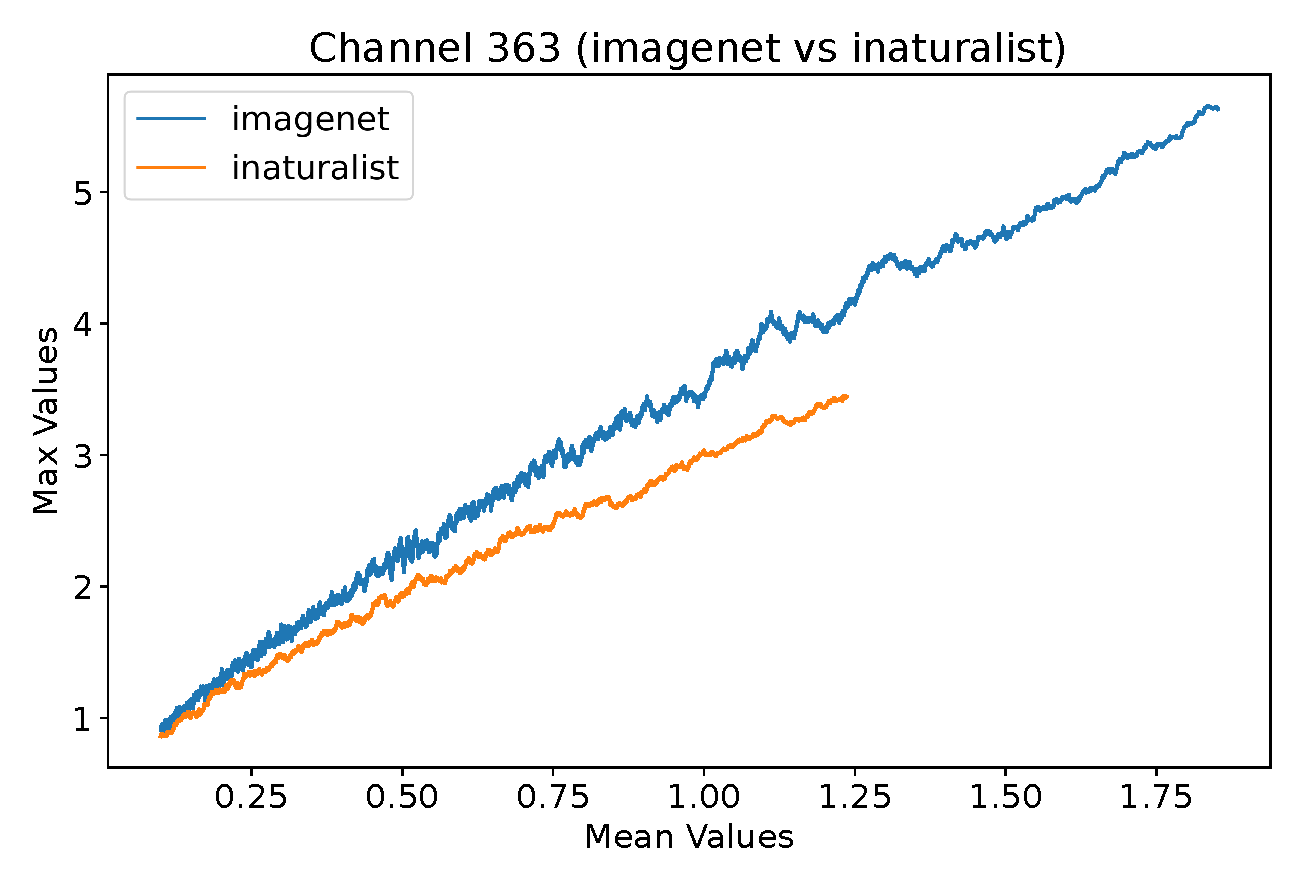
\includegraphics[width=0.24\linewidth]{eps/ap_re_channel_363.eps}
    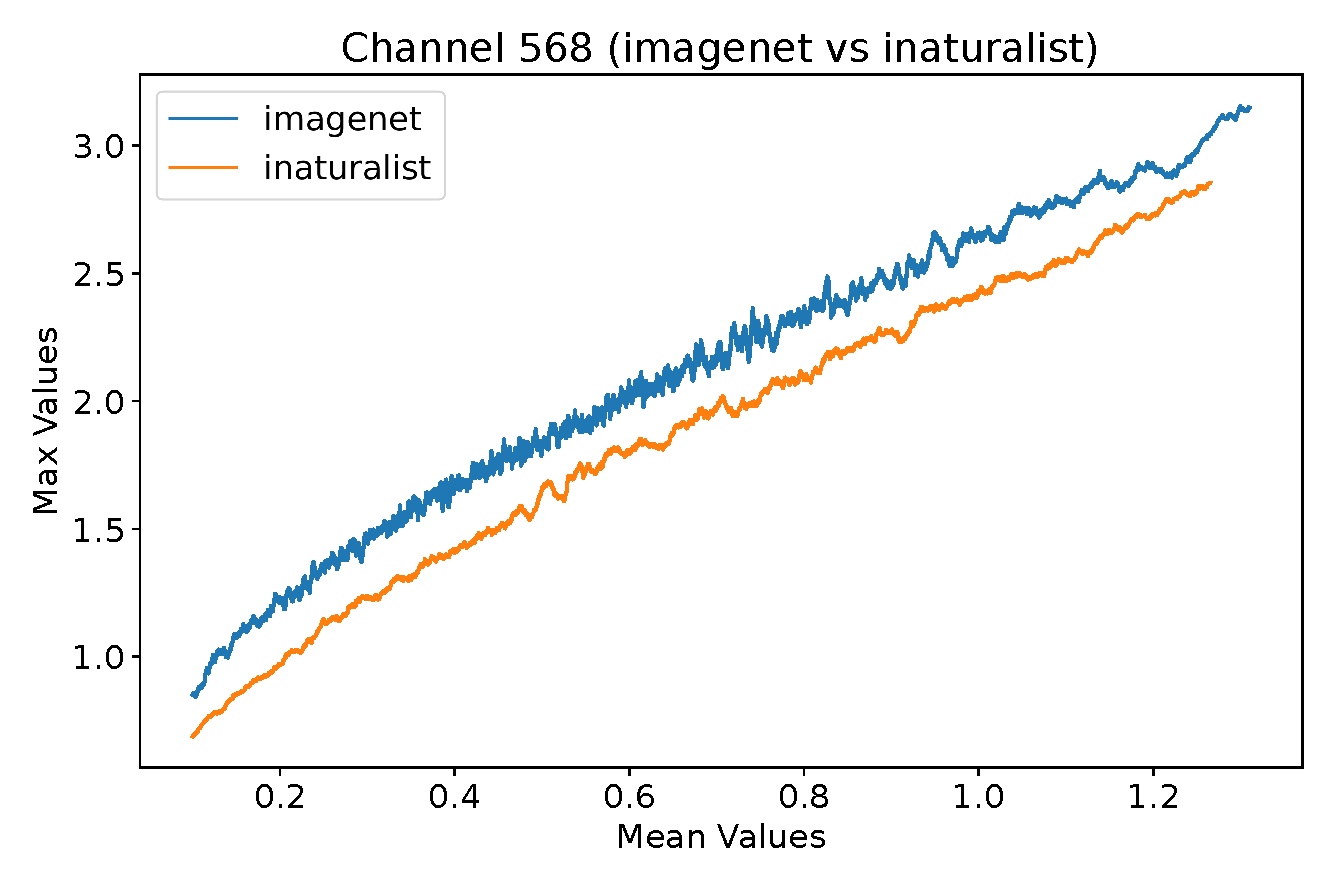
\includegraphics[width=0.24\linewidth]{eps/ap_re_channel_568.eps}
    \label{fig:resnet-r2}
  \end{subfigure}

  \caption{\textbf{Activation distribution at penultimate layer before global pooling operation within the ResNet50~\cite{he2016deep} architecture applied to ImageNet-1k and iNaturalist datasets~\cite{van2018inaturalist}.} We only include data points with an average activation over $0.1$. The figures show that our Neural Activation Prior (NAP) method is also effective in ResNet50, proving that NAP can be applied to different architectures.}
  \label{fig:appendix-e-resnet}
\end{figure}

\begin{figure}[!h]
  \centering
  \begin{subfigure}{\linewidth}
    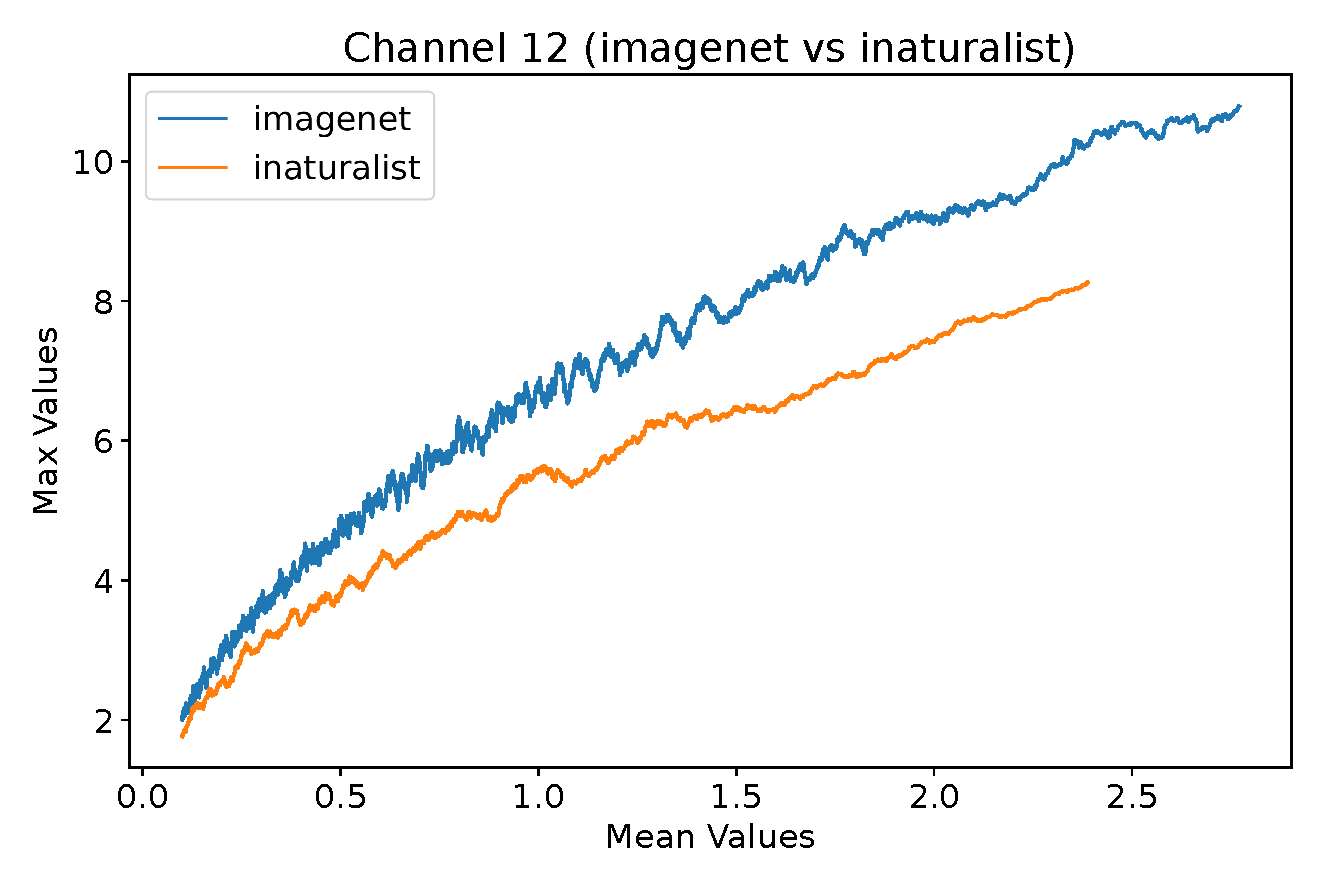
\includegraphics[width=0.24\linewidth]{eps/ap_vg_channel_12.eps}
    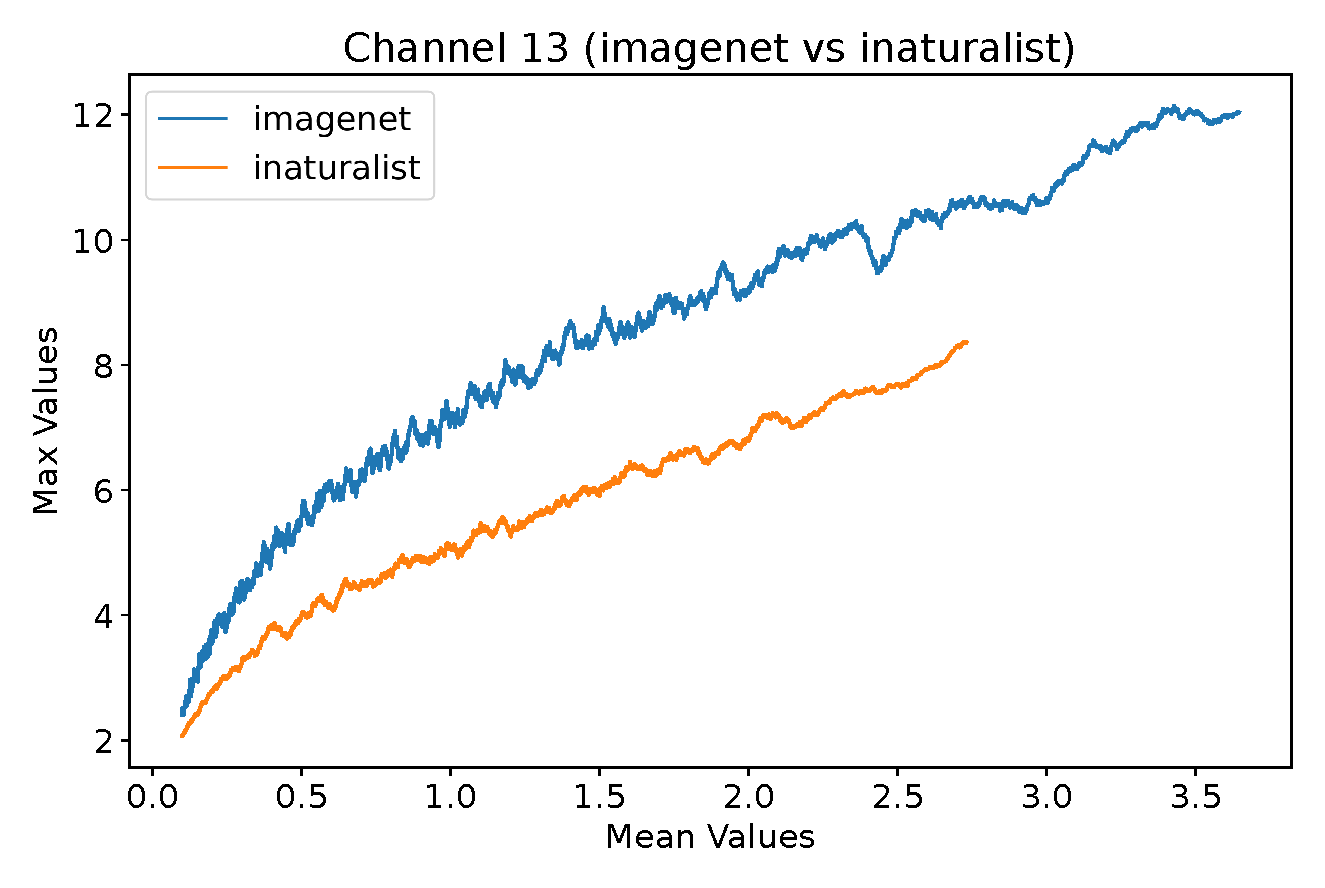
\includegraphics[width=0.24\linewidth]{eps/ap_vg_channel_13.eps}
    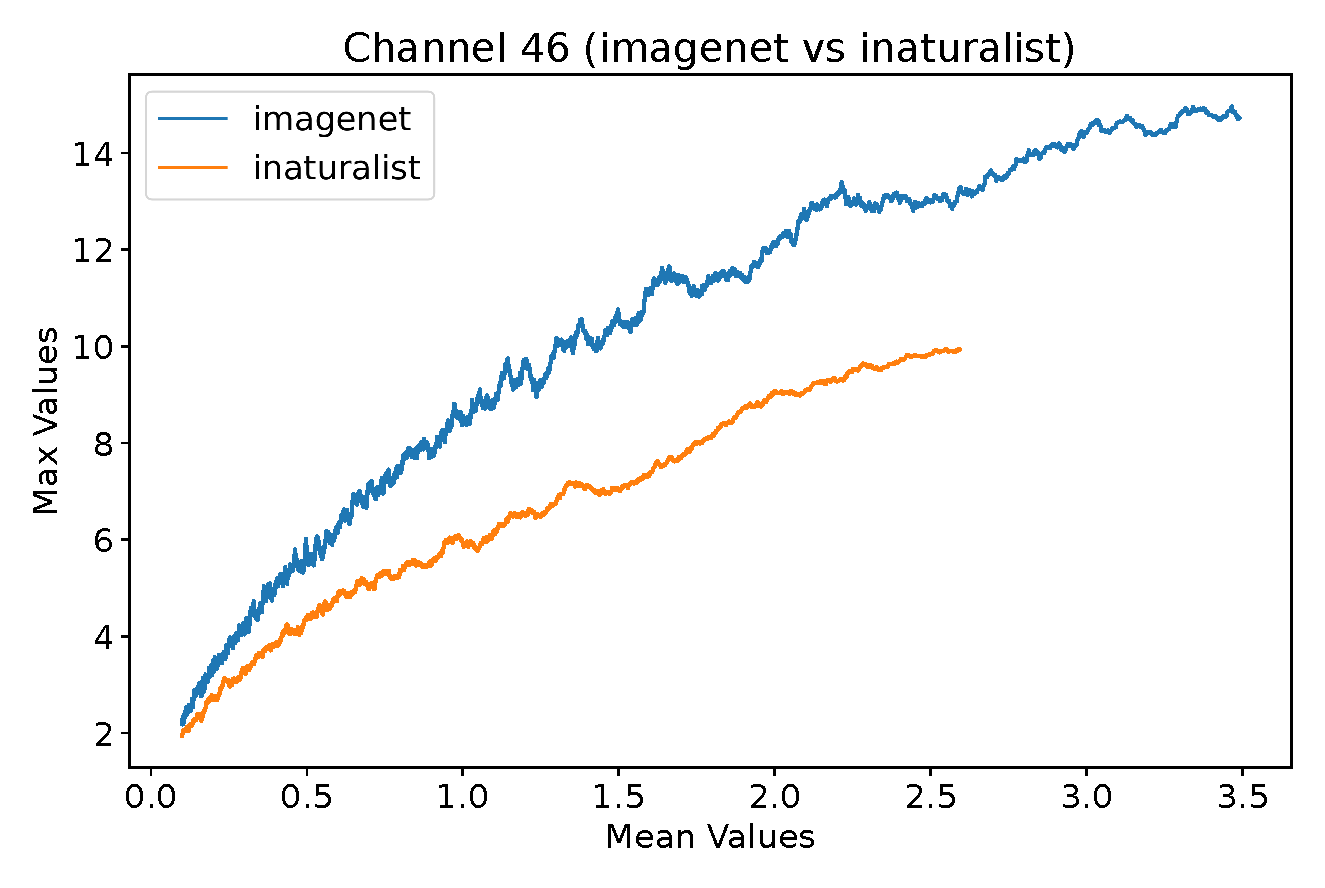
\includegraphics[width=0.24\linewidth]{eps/ap_vg_channel_46.eps}
    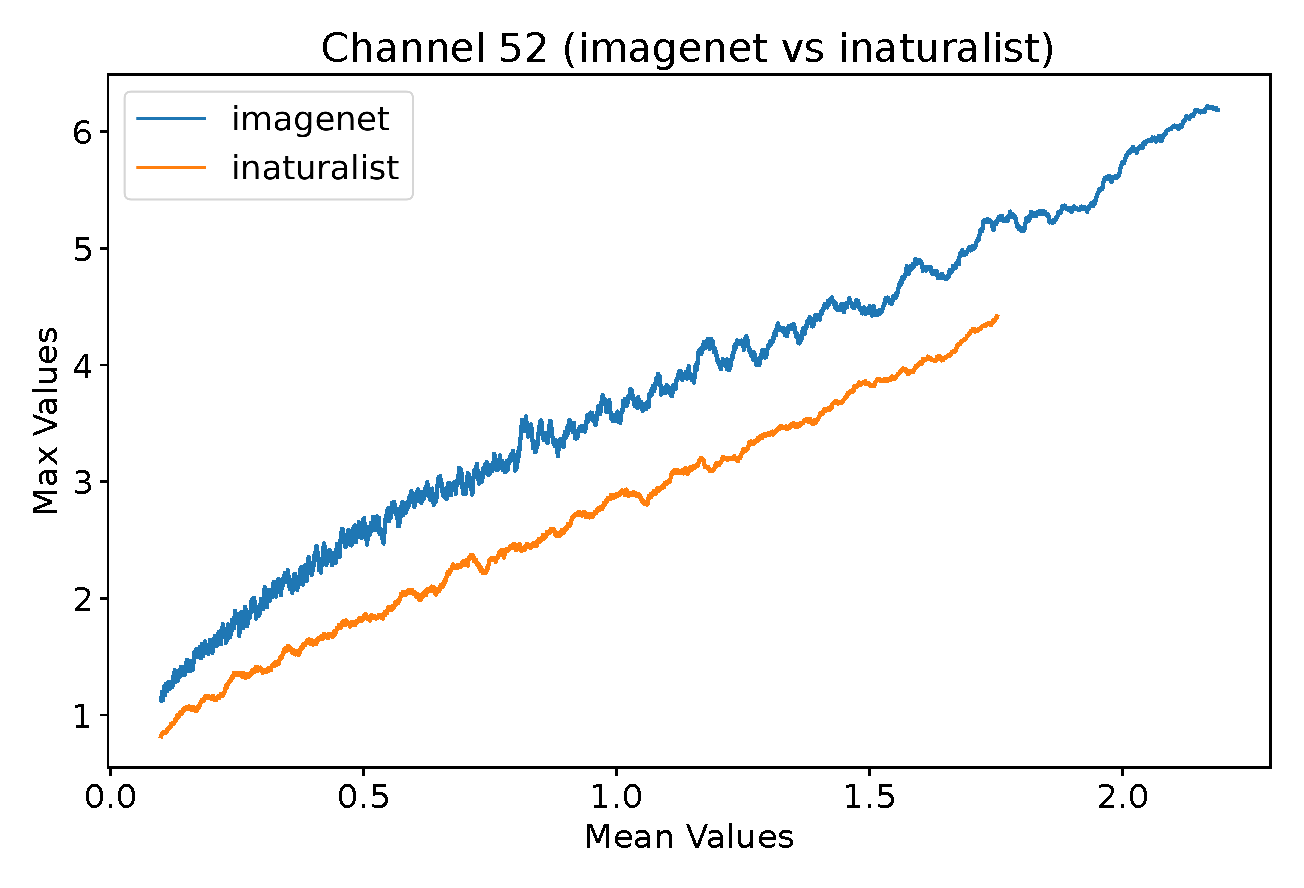
\includegraphics[width=0.24\linewidth]{eps/ap_vg_channel_52.eps}
    \label{fig:vgg-r1}
  \end{subfigure}

  \begin{subfigure}{\linewidth}
    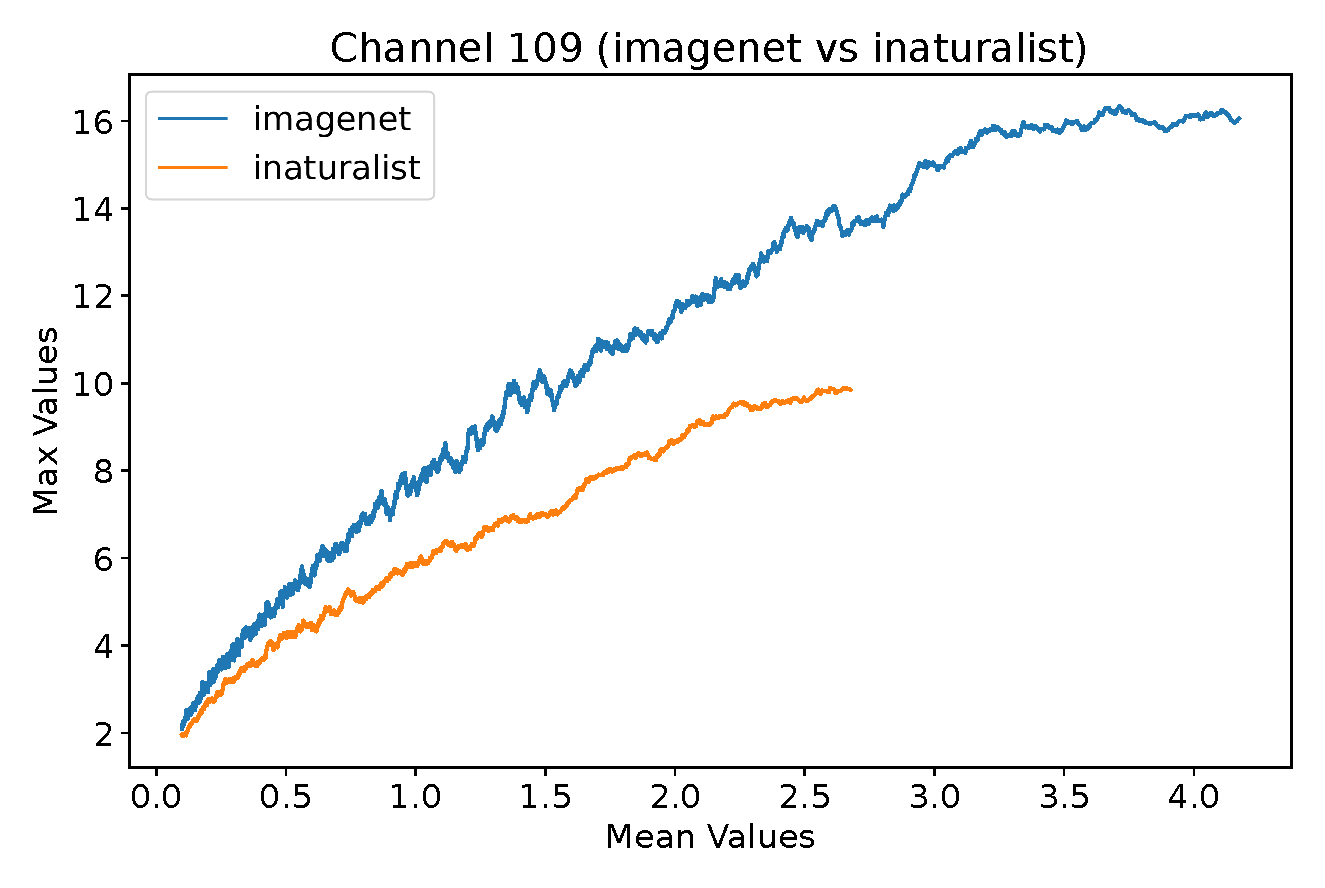
\includegraphics[width=0.24\linewidth]{eps/ap_vg_channel_109.eps}
    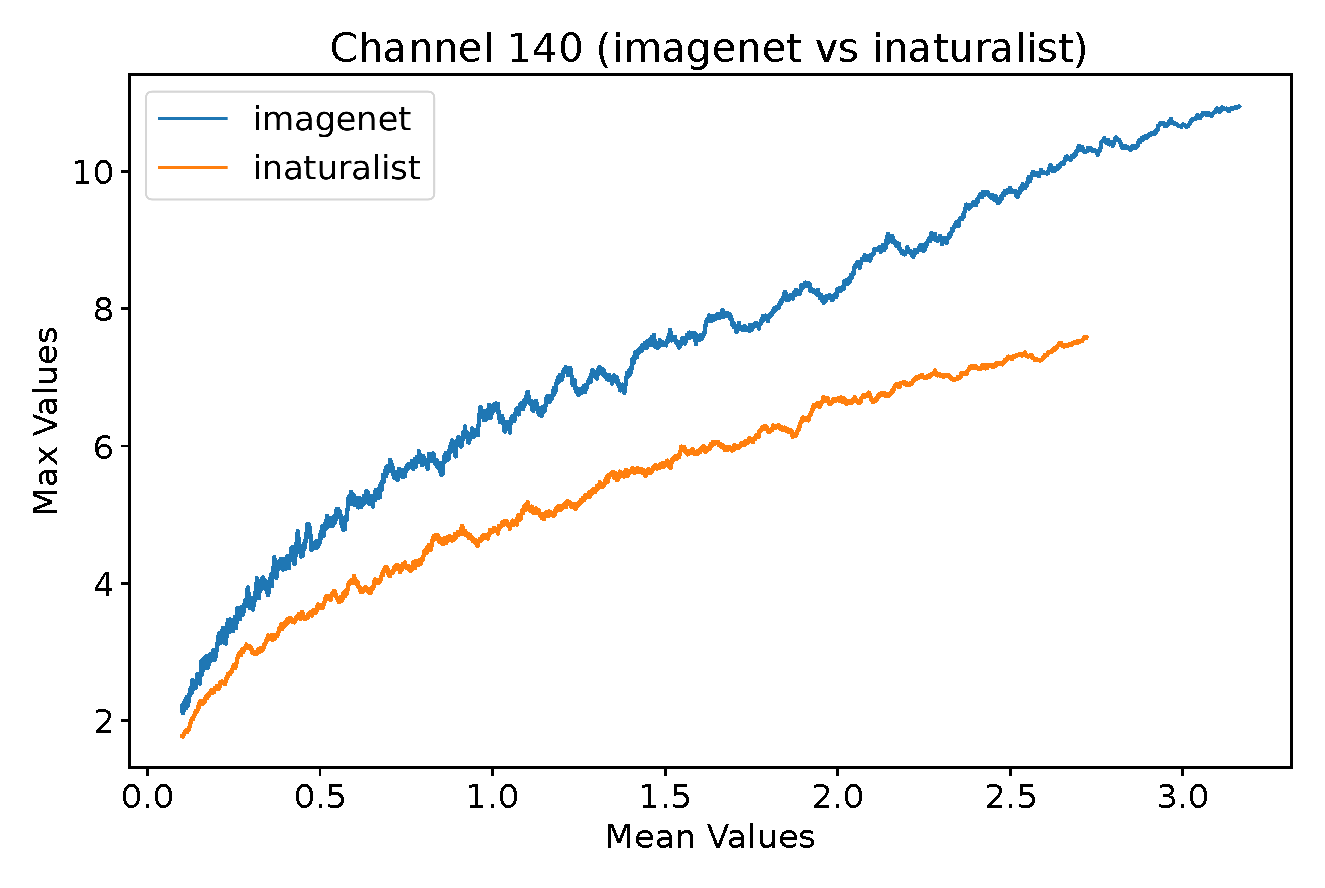
\includegraphics[width=0.24\linewidth]{eps/ap_vg_channel_140.eps}
    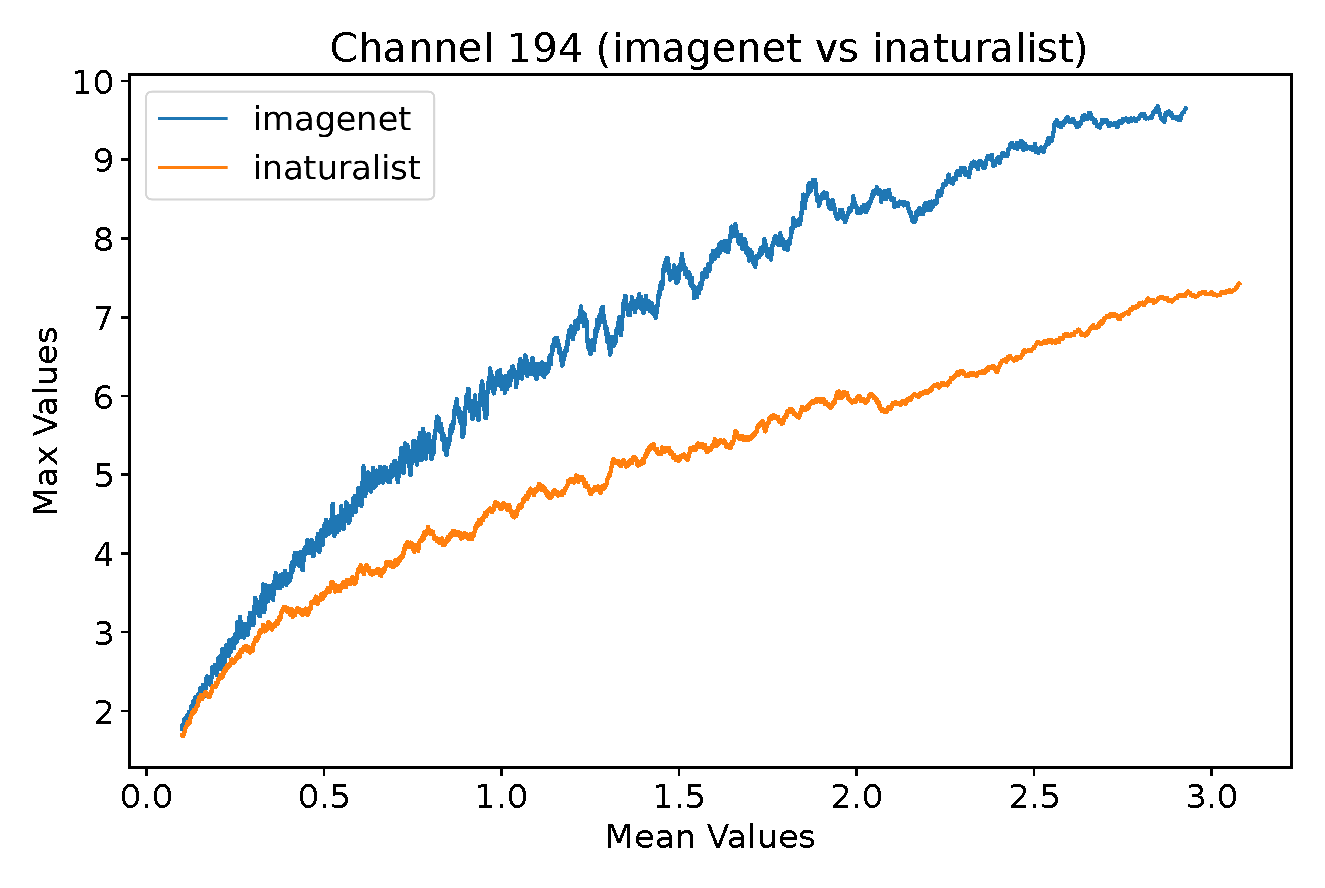
\includegraphics[width=0.24\linewidth]{eps/ap_vg_channel_194.eps}
    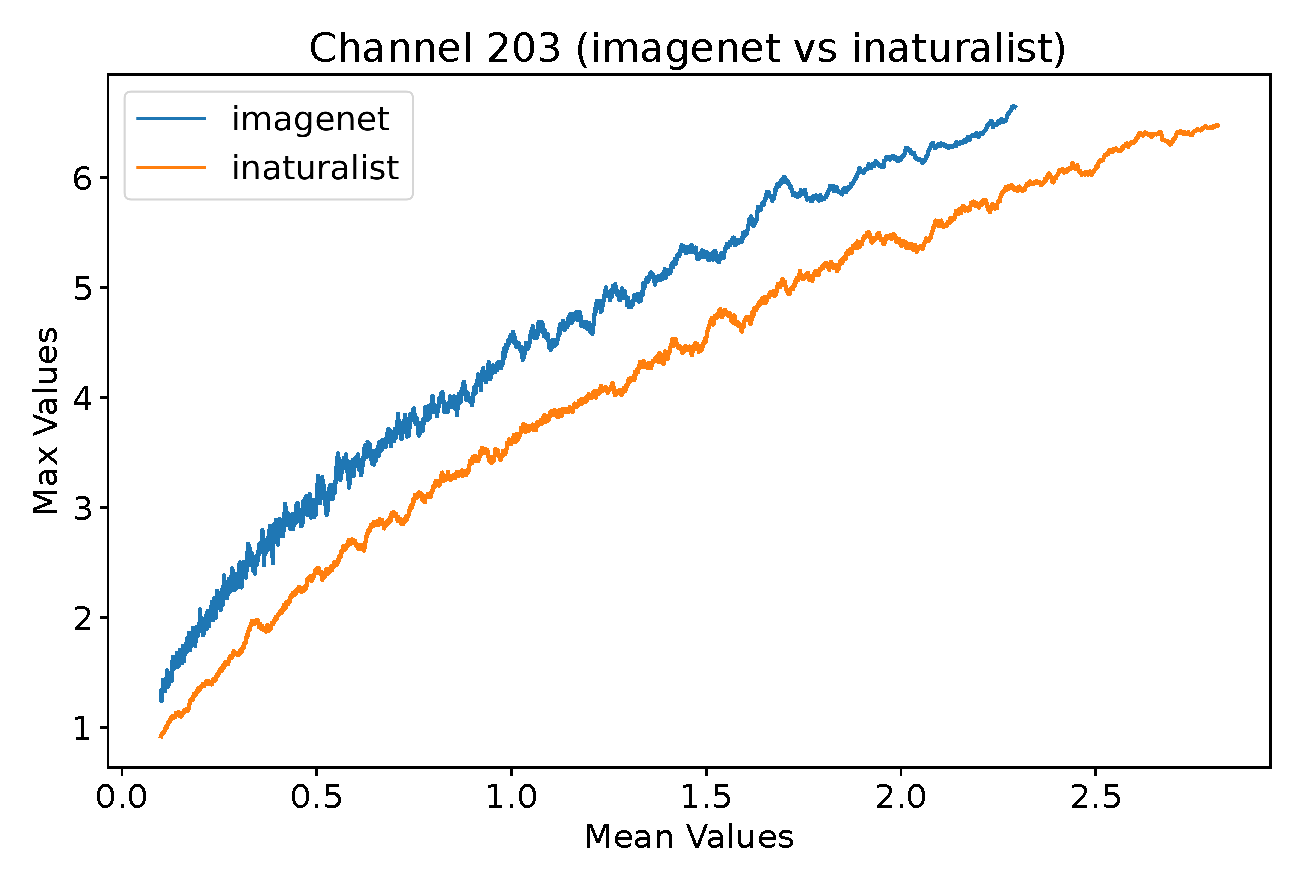
\includegraphics[width=0.24\linewidth]{eps/ap_vg_channel_203.eps}
    \label{fig:vgg-r2}
  \end{subfigure}

  \caption{\textbf{Activation distribution at penultimate layer before global pooling operation within the VGG16~\cite{simonyan2015very} architecture applied to ImageNet-1k and iNaturalist datasets~\cite{van2018inaturalist}.} We only include data points with an average activation over $0.1$. The figures show that our Neural Activation Prior (NAP) method is also effective in VGG16, proving that NAP can be applied to different architectures.}
  \label{fig:appendix-e-vgg}
\end{figure}

\section{Discussion}
\label{appendix:discuss}
Based on the ultra effectiveness of our prior, shown in the visualization results presented in Figure 1 in the main text and Figure~\ref{fig:appendix-e-mobilenet}, \ref{fig:appendix-e-resnet}, and \ref{fig:appendix-e-vgg} in this appendix, we are confident that more effective scoring functions exist. 
Due to space limitations, the primary focus and contribution of this paper is to introduce  this prior and and validate its effectiveness by proposing a new score function.
We leave the development of optimal scoring functions based on our prior for future work, aiming to further contribute to the community. We also hope this paper could encourage the researchers in  this community to build upon our work and advance the field.
\section{Licenses for existing assets}
\label{appendix:license}
We use several datasets and external code libraries in our research. To maintain anonymity, explicit references and detailed license information are not included in the submitted code. However, all creators and original owners of these assets are properly credited, and their licenses and terms of use are respected. The datasets used include CIFAR-10~\cite{krizhevsky2009cifar}, CIFAR-100~\cite{krizhevsky2009cifar}, ImageNet-1k~\cite{deng2009imagenet}, CIFAR-10-C~\cite{hendrycks2018corp}, CIFAR-100-C~\cite{hendrycks2018corp}, ImageNet-1k-C~\cite{hendrycks2018corp}, SVHN~\cite{netzer2011svhn}, iSUN~\cite{xu2015isun}, LSUN~\cite{yu2015lsun}, LSUN-crop~\cite{yu2015lsun}, iNaturalist~\cite{van2018inaturalist}, SUN~\cite{xiao2010sun}, Places~\cite{zhou2017places}, Textures~\cite{cimpoi2014texture}, and Places365~\cite{zhou2017places}. We also utilize DenseNet~\cite{huang2017densely}, ResNet~\cite{he2016deep}, VGG~\cite{simonyan2015very}, and ViT~\cite{dosovitskiy2020image} architectures in our experiments.
Our codebase for Neural Activation Prior (NAP) includes original code under the MIT License, with additional components from other sources. External code sources include ASH~\cite{djurisic2022extremely}, DICE~\cite{sun2022dice}, and~\cite{sun2022knn} under the MIT License.

\clearpage